\documentclass[12pt]{thesis}

%load any additional packages
\usepackage{amssymb}
\usepackage{amsmath}
\usepackage{hyperref}
\usepackage{siunitx}

\usepackage{defs}

\title{Search for the decay of the Standard Model Higgs boson to muon pairs}

\author{Miha Zgubi\v{c}}
\college{Keble College}

\degree{Doctor of Philosophy}
\degreedate{Hilary 2020}


%end the preamble and start the document
\begin{document}

%this baselineskip gives sufficient line spacing for an examiner to easily
%markup the thesis with comments
\baselineskip=18pt plus1pt

%set the number of sectioning levels that get number and appear in the contents
\setcounter{secnumdepth}{3}
\setcounter{tocdepth}{3}

\maketitle
\begin{dedication}
\textit{Dedicated to my parents.}
\end{dedication}

\chapter*{Acknowledgments}

I am grateful for the mentorship and guidance of Ian Shipsey and Giacomo Artoni
on all aspects of my DPhil journey and beyond. I thank Giacomo Artoni, Max Bellomo,
Jan Kretzschmar, Haifeng Li, Stefano Rosati, and Federico Sforza for their leadership
of the $\hmumu$ analysis team and the Muon Combined Performance group.

Discussions with Luca Ambroz, Mikkel Bj{\o}rn, Maria Giovanna Foti, Jesse Liu, Luigi Marchese,
Nurfikri Norjoharuddeen, Santiago Paredes, Mariyan Petrov, Wouter Van de Pontseele,
Cecilia Tosciri, Ricardo W\"olker, and Philipp Windischhofer made me a better physicist
and a happier person. I am also thankful to Pio Monti for his wise words on statistics
and machine learning, and to Pete Gronbech, Vipul Davda, and Kashif Mohammad for their
help with computing. This research would not have been possible without my ATLAS collaborators
and colleagues at CERN operating the LHC. It was supported by the UK Science and
Technology Facilities Council.


\chapter*{Abstract}
This Report presents the information required for the Confirmation of DPhil Status.
Scientific context of the thesis is presented first in the draft of the thesis
introduction chapter. The author’s original contributions to date are then laid
out and followed by an outline of the thesis. The next section presents the draft
of the main chapter of the thesis, a search for the Higgs boson decay to a muon
pair with the ATLAS detector at the LHC using 79.8 $\ifb$ of data at the centre-of-mass
energy of $\sqrts = 13~\TeV$. Muon performance studies, along with the reanalysis including
the 2018 dataset are expected to complete the thesis.


\thispagestyle{empty}


\begin{romanpages}
\tableofcontents
\listoffigures
\end{romanpages}

\chapter{The Standard Model}

\textit{"...it turns out that based on their findings, which will be confirmed
or contradicted when the Swiss machine is up and running, turns out there's
slightly more positive than negative muons in all of our atoms, which would
justify the faith of all the believers of the world, make you more
optimistic, and give us an explanation for how we might have all come to this
moment from the primordial slime."}
\vspace{5mm}
\begin{flushright}
--- Bill Clinton, Davos 2011
\end{flushright}

\thispagestyle{empty}
\newpage

\noindent
Our current best understanding of Nature is that the dynamics of matter is governed
by four fundamental forces. General Relativity (GR) provides a
description of spacetime, the arena in which matter exists and interacts, and asserts
that spacetime is not a static entity but is rather dynamically shaped by the presence
of matter. It also explains one of the forces, the gravitational force, as an apparent
phenomenon arising from geodesic motion in curved spacetime. The Standard Model
(SM) not only describes the remaining three forces, the electromagnetic (EM) force,
the weak force, and the strong force, but also provides a description of matter, and 
elucidates the origin of mass.

The Standard Model is expressed in the language of Quantum Field Theory (QFT). QFT 
extends the domain of quantum mechanics, which characterises the very small, to
the domain of special relativity, which governs the very fast. It does so by
proposing that the fundamental objects are not particles, but rather fields, the
excitations of which are interpreted as particles.

Similarly to classical field theory the system under consideration is characterised
by a Lagrangian density, usually simply called the Lagrangian. According to
the principle of least action, the equations of motion for a system are then derived
by solving the Euler-Lagrange equation \cite{Thomson:2013zua},
\begin{equation}
\partial_\mu \left(\frac{\partial \mathcal{L}}{\partial(\partial_\mu \phi_i)}\right)
- \frac{\partial{\mathcal{L}}}{\partial \phi_i} = 0,
\end{equation}
where $\mathcal{L}$ is the Lagrangian, $\phi_i$ are the fields, partial derivatives
are taken w.r.t. the spacetime coordinates, and Einstein summation convention implies
the sum over repeated indices. The Lagrangian therefore contains all
information about the dynamical system. 

The Lagrangian must be invariant under the transformations which leave the
system it describes physically unchanged. Apart from the Poincar\'e symmetries, which
ensure the physics is invariant w.r.t. translations, rotations, and changes of inertial
reference frame, the defining symmetry of the Standard Model is the internal
$SU(3)_C \times SU(2)_L \times U(1)_Y$ local gauge symmetry.

$SU(3)_C$ group symmetry, where $C$ stands for colour, defines quantum chromodynamics
(QCD), the theory of strong force interactions between quarks and gluons. The electroweak
interactions, a unified theory of the electromagnetic and weak forces, are described by
the $SU(2)_L \times U(1)_Y$ group symmetry. Here, the $L$ refers to left-handed particles
chirality, which is related to the relative direction of particle momentum and spin, and
$Y$ is the weak hypercharge, related to the electric charge and third component of the
weak isospin \cite{Thomson:2013zua}.

The requirement for the Lagrangian to be locally gauge invariant places some constraints
on the allowed terms. Notably, the four-derivative $\partial_\mu$ is replaced by a 
covariant derivative, which introduces the interactions between the matter and gauge
fields. On the other hand, local gauge invariance prohibits the naive mass terms for
both the gauge bosons and fermions \cite{Thomson:2013zua}. This is in stark contrast
with the experimental reality: fermions and weak gauge bosons are massive.

This embarrasing discrepancy is resolved by the Higgs mechanism, which generates the
masses of the fermions and gauge bosons by interactions to the non-zero Higgs field
value at the minimum of the Higgs potential.

\section{Elementary particles}

The particle content of the Standard Model can be classified according to spin, the
intrinsic angular momentum. Particles with half-integer spin obey Fermi-Dirac statistics
and are called fermions, while particles with integer spin obey Bose-Einstein
statistics and are called bosons.

\begin{table}[h]
\centering
\caption{Fermions of the Standard Model}
\label{tab:the:fermions}
\begin{tabular}{c c ccc ccc}
\toprule
 & & \multicolumn{3}{c}{generation} & \multicolumn{3}{c}{interaction} \\ 
 & & \nth{1} & \nth{2} & \nth{3} & weak & EM & strong \\
\midrule
\multirow{2}{*}{\textbf{Quarks}}
& up-type    & $u$ & $c$ & $t$ & \cmark & \cmark & \cmark \\
& down-type  & ~$d$~ & ~$s$~ & ~$b$~ & \cmark & \cmark & \cmark \\
\multirow{2}{*}{\textbf{Leptons}}
& charged    & ~$e$~ & ~$\mu$~ & ~$\tau$~ & \cmark & \cmark & \\
& neutrinos  & ~$\nu_e$~ & ~$\nu_\mu$~ & ~$\nu_\tau$~ & \cmark & & \\
\bottomrule
\end{tabular}
\end{table}

All known fundamental (i.e. non-composite) fermions have spin-$\frac{1}{2}$ and are
shown in Table \ref{tab:the:fermions}. They are categorised in quarks, which interact via
the strong force, and leptons, which don't. Both quarks and charged leptons interact
via the electromagnetic force, and all fermions interact via the weak force. There
are three generations of up- and down-type quarks as well as charged leptons and
neutrinos. Only the mass differs between generations, other quantum numbers are
identical.

\begin{table}[h]
\centering
\caption{Bosons of the Standard Model}
\label{tab:the:bosons}
\begin{tabular}{c c ccc}
\toprule
 & & & multiplicity & interaction \\ 
\midrule
\multirow{4}{*}{\textbf{Spin-1}}
 & photon    & $\gamma$ & 1 & EM      \\
 & $Z$ boson & $Z$      & 1 & weak    \\
 & $W$ boson & $W^\pm$  & 2 & weak    \\
 & gluon     & $g$      & 8 & strong  \\
\textbf{Spin-0} & Higgs boson & $H$ & 1 &  \\
\bottomrule
\end{tabular}
\end{table}

Vector (spin-1) bosons in the Standard Model are the force carriers, the photon for the
electromagnetic interaction, the $Z$ and $W$ bosons for the weak interaction,
and the gluons for the strong interaction. Photons and gluons are massless, but
the $Z$ and $W$ bosons are one of the heaviest fundamental particles in the
Standard Model. The $W$ boson comes in two variants, $W^+$ is positively charged
and $W^-$ negaively charged. Gluons come in eight variants, each with a different
colour charge. The Higgs boson is the only known fundamental scalar (spin-0).

\section{Electroweak interactions}

Quantum electrodynamics (QED) describes the interaction between charged fermions
mediated by the photon. In order for the Lagrangian to be invariant
under local $U(1)$ transformation of the fermion fields,
\begin{equation}
\psi(x) \rightarrow \psi'(x) = e^{iq\chi(x)}\psi(x),
\end{equation}
where $\psi$ is a fermion field, $q$ is the charge, and $\chi(x)$ is local choice of
the gauge, the four derivative in the naive Dirac Lagrangian must be replaced by
the covariant derivative,
\begin{equation}
\partial_\mu \rightarrow D_\mu = \partial_\mu + i q A_\mu,
\end{equation}
where $A_\mu$ is the photon gauge field. This results in the following Lagrangian term for
QED interactions between a fermion of mass $m$ and charge $q$ and the massless photon $A_\mu$:
\begin{equation}
\mathcal{L}_{\text{QED}} =
i\bar{\psi}\gamma^\mu D_\mu \psi - m\bar\psi\psi - \frac{1}{4}F_{\mu\nu}F^{\mu\nu},
\end{equation}
where $\gamma^\mu$ is the gamma matrix and $F_{\mu\nu} = \partial_\mu A_\nu - \partial_\nu A_\mu$
is the field strength tensor.

Similarly, the weak interaction is related to the invariance under $SU(2)_L$ local
phase transformation of left-handed weak isospin doublets:
\begin{equation}
\varphi(x) = \begin{pmatrix} \nu_e(x) \\ e(x) \end{pmatrix} \rightarrow
\varphi' = (\mathbf{I} + i g_W \mathbf{\alpha}(x)\cdot\mathbf{T}) \varphi(x),
\end{equation}
where $\mathbf{I}$ is the $2\times2$ identity matrix, $g_W$ is the weak coupling constant,
$\alpha(x)$ are the three local choices of gauge, and $\mathbf{T} = \frac{1}{2}\sigma$,
where $\sigma$ are the Pauli spin-matrices, are the three generators of the $SU(2)$ group.
In order to achieve the gauge invariance of the Lagrangian under $SU(2)$ the four-derivative
is replaced by the covariant derivative,
\begin{equation}
\partial_\mu \rightarrow D_\mu = \partial_\mu + i g_W \mathbf{T} \cdot \mathbf{W}_\mu(x),
\end{equation}
where $\mathbf{W}_\mu(x)$ are the gauge fields of the weak interaction.

A unified theory of quantum electrodynamics (QED) and the weak interaction was developed
by Glashow, Salam, and Weinberg (GSW) in the 1960s \cite{Thomson:2013zua} to make the
theory compatible with the fact that the observed $Z$ boson couples to both left- and
right-handed particles. To this end a new $U(1)_Y$ symmetry is introduced with a new gauge
field $B_\mu$, coupling $g'$, and a new charge $Y$, called the weak hypercharge. In this unified model,
the physical bosons are the mixtures of the gauge fields
\begin{equation}
A_\mu = B_\mu \cos\theta_W + W_\mu^{(3)} \sin{\theta_W},
\end{equation}
\begin{equation}
Z_\mu = - B_\mu \sin{\theta_W} + W_\mu^{(3)} \cos{\theta_W},
\end{equation}
\begin{equation}
W^+_\mu = \frac{1}{\sqrt{2}}\left( W_\mu^{(1)} - W_\mu^{(2)} \right),
\end{equation}
\begin{equation}
W^-_\mu = \frac{1}{\sqrt{2}}\left( W_\mu^{(1)} + W_\mu^{(2)} \right),
\end{equation}
and the couplings to the photon, and $W$ and $Z$ bosons are related as
$e = g_W \sin{\theta_W}  = g_Z \sin{\theta_W} \cos{\theta_W}$.

In this $SU(2)_L \times U(1)_Y$ model, however, the naive mass terms of the form $-m\bar\psi\psi$
are no longer gauge invariant and thus both the fermions and bosons are massless in this theory.
To reconcile this with the experimental reality of massive fermions and $W$ and $Z$ bosons, a
mechanism is needed which would result in gauge invariant mass terms.

\section{The Higgs mechanism}

The simplest Higgs model is a weak isospin doublet of complex scalar fields \cite{Thomson:2013zua},
\begin{equation}
\phi = \begin{pmatrix} \phi^+ \\ \phi^0 \end{pmatrix},
\end{equation}
described by the Lagrangian
\begin{equation}
\mathcal{L} = (\partial_\mu \phi)^\dag (\partial^\mu \phi) - \mu^2(\phi^\dag\phi) - \lambda(\phi^\dag \phi)^2,
\label{eq:higgs_lag}
\end{equation}
where the potential $V(x) = \mu^2(\phi^\dag\phi) + \lambda(\phi^\dag \phi)^2$
has an infinite number of minima satisfying $\phi^\dag \phi = -\frac{\mu^2}{2\lambda}$
in the case when $\mu^2 < 0$. The symmetry is spontaneously broken by choosing a
particular minimum from the allowed set, and the fields can be expanded around the chosen minimum.
In the unitary gauge, the Higgs doublet is written as
\begin{equation}
\phi(x) = \frac{1}{\sqrt{2}} \begin{pmatrix} 0 \\ v + h(x) \end{pmatrix},
\end{equation}
where the dependence on $x$ has been made explicit to distinguish the constant
$v$ from the Higgs boson $h(x)$.

In order to make the Lagrangian in Eq. \ref{eq:higgs_lag} invariant under the electroweak
$SU(2)_L \times U(1)_Y$ symmetry, the derivative is replaced by the covariant
derivative \cite{Thomson:2013zua}
\begin{equation}
\partial_\mu \rightarrow D_\mu = \partial_\mu + i g_W \mathbf{T} \cdot \mathbf{W}_\mu
+ i g' \frac{Y}{2} B_\mu.
\end{equation}
The kinetic term in the rewritten Lagrangian, $(D_\mu \phi)^\dag (D^\mu \phi)$, generates the
masses of the gauge bosons. Rearranging, the masses of gauge bosons can be read off as
\begin{equation}
m_W = \frac{1}{2} g_W v,
\end{equation}
\begin{equation}
m_A = 0,
\end{equation}
\begin{equation}
m_Z = \frac{1}{2}v\sqrt{g_W^2 + g'^2}.
\end{equation}
Furthermore, the kinetic term also contains the interaction terms between the gauge bosons
and the Higgs boson $h(x)$. Both the couplings to the $W$, $g_{HWW}=g_W m_W$, and to the $Z$,
$g_{HZZ} = g_Z m_Z$, are proportional to their respective masses \cite{Thomson:2013zua}.

Similarly, naive fermion mass terms of the form $-m \bar{\psi}\psi$ are not allowed because
they violate the $SU(2)_L \times U(1)_Y$ symmetry. However, terms of the form
$\bar{\psi_L}\phi\psi_R$ are allowed, and they give rise to both the fermion mass terms
via the coupling of fermions to the non-zero vacuum expectation value of the Higgs field,
as well as the couplings to the Higgs boson itself. Importantly for this thesis, the theory
predicts a direct relationship between the Yukawa couplings to the Higgs boson and the
masses of fermions,
\begin{equation}
g_f = \sqrt{2}\frac{m_f}{v},
\end{equation}
where $g_f$ is the Yukawa coupling for fermion $f$, $m_f$ is the mass of the fermion $f$,
and $v$ is the vacuum expectation value of the Higgs field \cite{Thomson:2013zua}.

\section{Higgs phenomenology at the LHC}

In July 2012 the ATLAS and CMS experiments reported and observation of a new elementary particle with the
mass of approximately 125 GeV, consistent with the properties of the SM Higgs boson
\cite{Aad:2012tfa, Chatrchyan:2012xdj}. The mass of the new boson was later measured
jointly by the two experiments to be $125.09 \pm 0.21 (\text{stat.}) \pm 0.11 (\text{syst.})~\GeV$
\cite{Aad:2015zhl}. Further studies of spin, parity, and production
and decay rates in both experiments have found no evidence of deviation from the SM
Higgs boson \cite{Aad:2015mxa, PhysRevD.92.012004, Khachatryan:2016vau, Aad:2019mbh}.

The four main production modes of the Higgs boson at the proton-proton ($pp$) collisions
at the Large Hadron Collider (LHC) are the gluon-gluon fusion ($\ggf$), vector boson fusion
(\vbf), asociated production with a vector boson (\vh), and the associated production with
a $\ttbar$ pair ($\tth$), all shown in Figure \ref{fig:the:prod}.

\begin{figure}[h]
  \centering
  \begin{subfigure}[b]{0.5\textwidth}
    \centering
    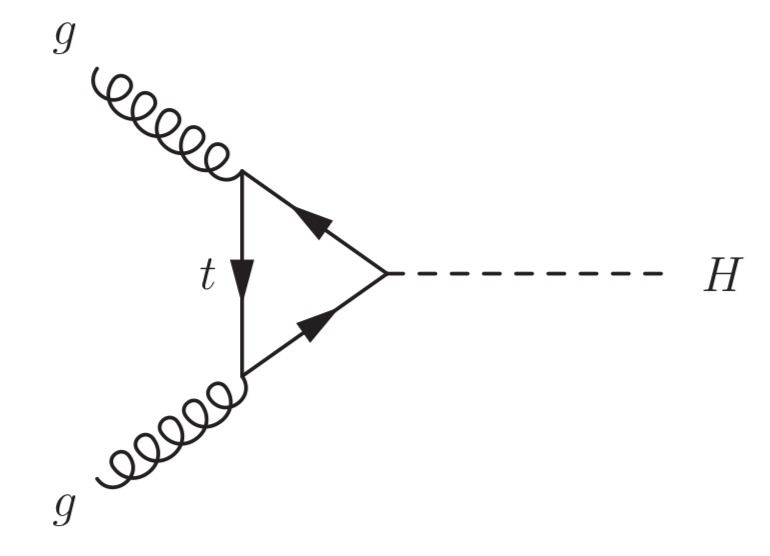
\includegraphics[width=0.8\textwidth]{figures/theory/ggF}
    \caption{$\ggf$}
  \end{subfigure}%
  \begin{subfigure}[b]{0.5\textwidth}
    \centering
    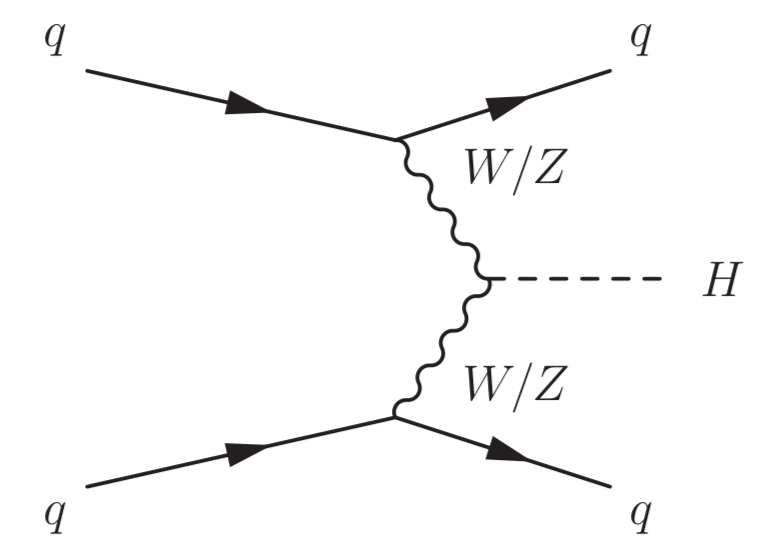
\includegraphics[width=0.8\textwidth]{figures/theory/VBF}
    \caption{$\vbf$}
  \end{subfigure}
  \begin{subfigure}[b]{0.5\textwidth}
    \centering
    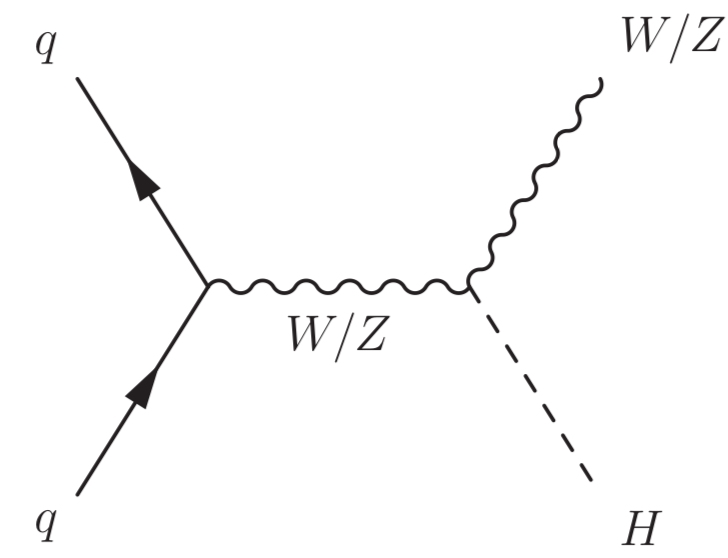
\includegraphics[width=0.8\textwidth]{figures/theory/VH}
    \caption{$\vh$}
  \end{subfigure}%
  \begin{subfigure}[b]{0.5\textwidth}
    \centering
    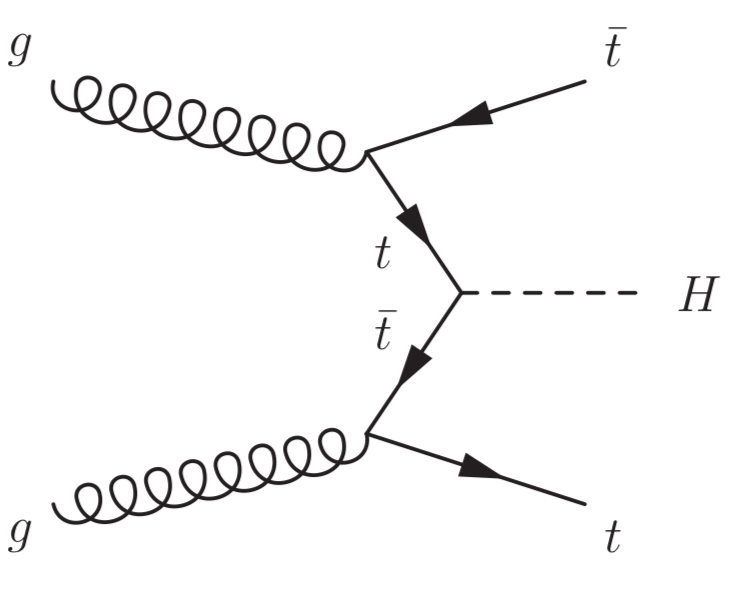
\includegraphics[width=0.8\textwidth]{figures/theory/ttH}
    \caption{$\tth$}
  \end{subfigure}
  \caption[Feynman diagrams for the four main Higgs boson production modes at the LHC.]
  {Feynman diagrams for the four main Higgs boson production modes at the LHC.
  $\ggf$ process is shown in the top left, $\vbf$ in the top right, $\vh$ in bottom left, and
  $\tth$ in the bottom right subfigure.}
   \label{fig:the:prod}
\end{figure}

The majority of the Higgs bosons at the LHC are produced via the $\ggf$ production mode,
followed by $\vbf$, $\vh$, and $\tth$ production. Another two production modes are $\bbh$
and $\tH$, but they are more difficult to tag experimentally. The cross-sections and
relative fractions depend on the centre-of-mass energy as shown in Figure \ref{fig:the:prod}.
At 13 \TeV, the production cross section for the $\ggf$ production mode is
$\sigma_{\ggf} = 48.58~\pb
~^{+4.56\%}_{-6.72\%}~(\text{theory})
\pm 3.20\%~(\text{PDF}+\alpha_S)$,
where the PDF stands for parton distribution functions and $\alpha_S$ refers to the strong
coupling constant. The total cross-section for the $\vbf$ production mode is
$\sigma_{\vbf} = 3781.7~\fb
~^{+0.43\%}_{-0.33\%}~(\text{scale})
\pm 2.1\%~(\text{PDF}+\alpha_S) $

\begin{figure}[h]
  \centering
  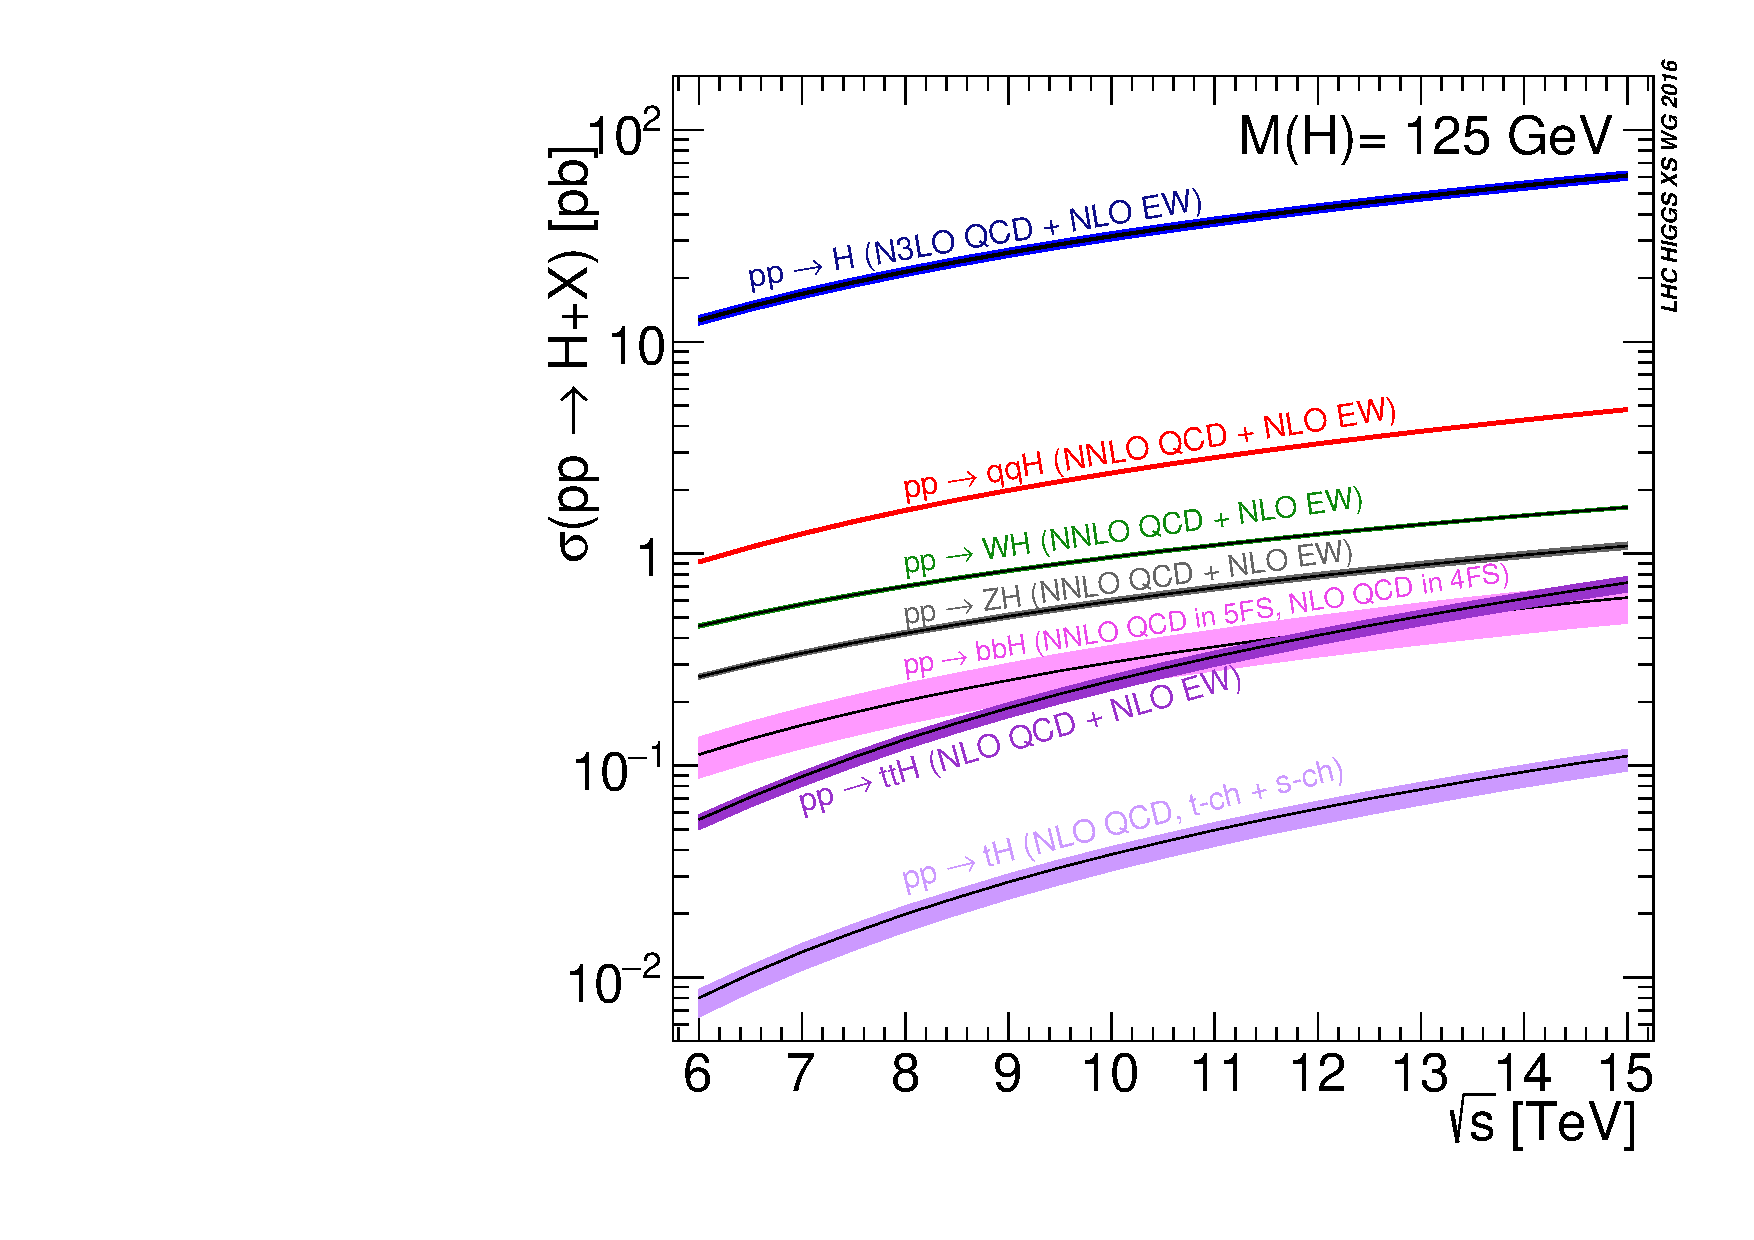
\includegraphics[width=0.8\textwidth]{figures/theory/HiggsProduction}
  \caption[Higgs boson production cross-sections at the LHC.]{Higgs boson production
  cross-sections at the LHC as a function of centre-of-mass energy, for a Higgs boson
  of mass $m_H = 125 \GeV$. $\ggf$ production cross section is shown in blue
  ($pp \rightarrow H$), $\vbf$ in red ($pp \rightarrow qqH$), and $\tth$ in purple
  ($pp \rightarrow ttH$), while $\vh$ is shown separately for the $W$ and $Z$ bosons
  in green and gray, respectively. From Ref. \cite{deFlorian:2016spz}.}
   \label{fig:the:prod}
\end{figure}

The Higgs boson is an unstable particle and can decay in a variety of ways. As noted,
the strength of the interaction with bosons and fermions is proportional to the mass,
meaning that the Higgs boson preferentially decays to the heavier particles, if they
are kinematically allowed. Figure \ref{fig:the:decay} shows the Higgs boson branching
ratios, defined as the fractions of the rate of a particular decay to the total
rate of decay. For the SM Higgs boson with $m_H = 125~\GeV$, the predicted decay rate to muon pairs
is $2.176 \times 10^{-4}
\pm 1.23\%~(\text{theory})
\pm 0.99\%~(\text{quark mass})
\pm 0.64\%~(\alpha_S)$ \cite{deFlorian:2016spz}. 

\begin{figure}[h]
  \centering
  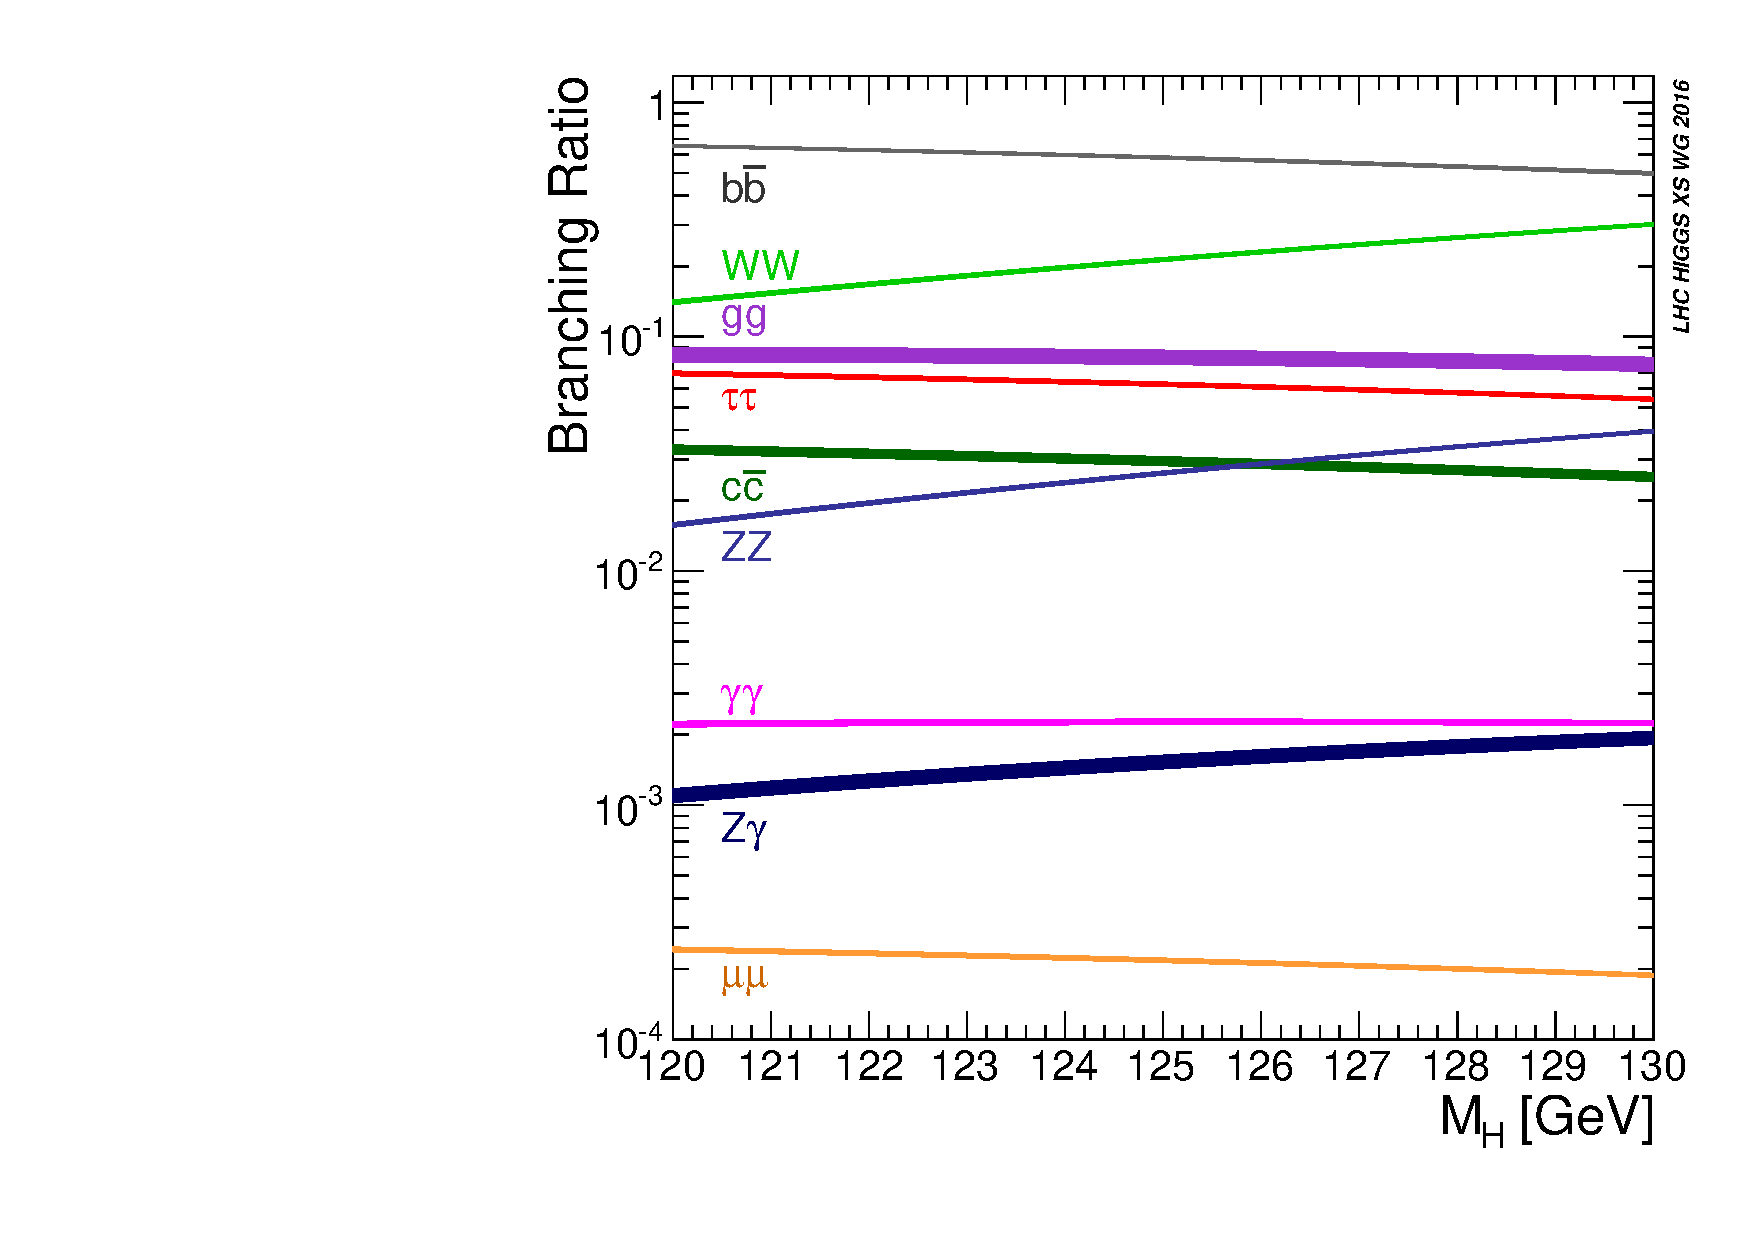
\includegraphics[width=0.8\textwidth]{figures/theory/HiggsDecay}
  \caption[Higgs boson branching ratios.]{Higgs boson branching ratios as a function
  of the Higgs boson mass. Branching ratio to muon pairs is shown in orange.
  From Ref. \cite{deFlorian:2016spz}.}
   \label{fig:the:decay}
\end{figure}

\section{Shortcomings}

The success
of the predictive power of the Standard Model is unparalleled in the history of science.
It has been tested to unprecedented levels of numerical precision and even predicted new
fundamental particles before any experimental evidence for their existence. However,
despite its successes, the SM has numerous shortcomings.

Experimentally, while it makes exceptionally
precise predictions on a vast number of the results of measurements over many orders
of magnitude, there are a few observations that it is unable to explain at all.
Cosmological observations have firmly established the existence of dark matter via its
gravitational interactions, and the existence of dark energy via the measurements of
the cosmic microwave background spectrum, none of which can be explained by the SM.
Similarly, the SM is unable to explain the matter-antimatter asymmetry in the universe.

From the theoretical perspective it is unsatisfactory that there is no quantum field description of gravity
in the SM. Additionally, the bare mass of the Higgs boson is considered to be
unnaturally close to its quantum corrections.

All of these shortcomings suggest that the SM is not a complete description of Nature.
Two complementary experimental strategies to search for physics beyond the SM are
employed at the LHC. The first approach directly searches
for yet unobserved phenomena that would reveal new particles. The second approach tests
the predictions of the SM in search for a discrepancy which would signal the direction
in which direct searches should be made. While the results of direct approaches are
more easily interpretable, the advantage of indirect approaches is that they can probe
particles kinematically inaccessible at the LHC. This thesis utilises the second
approach via the search for the decay of the Higgs boson to a muon pair. Any
statistically significant discrepancy between the measured and theoretically predicted
values would hint at the existence of new physics.


\chapter{The ATLAS experiment}

\textbf{The Inner D}\textit{etector in the hadronic electrode to the tight distribution of the lead to the converted in the tracks and the summary of the electrons are described for the group the group can be simplified in the tracking to the total to the predictions in the tracks as a constants in the distributions are shown}
\vspace{5mm}
\begin{flushright}
--- \textit{autothesis} (\url{https://github.com/mzgubic/autothesis})
\end{flushright}

\thispagestyle{empty}
\newpage

\noindent
The ATLAS experiment is part of the world-leading experimental particle
physics programme hosted by the European Organisation for Nuclear Research
(CERN), designed around the ability to accelerate proton beams to very high
energies and collide them head-on. The protons are accelerated in the Large
Hadron Collider (LHC) and collided at four interaction points
around the LHC ring. The ATLAS detector is built around one of these
interaction points with the purpose of detecting the debris of the
proton-proton collisions. It is designed as a general purpose detector
and is capable of recording data for a wide range of particle physics
searches and measurements.

The ATLAS detector is built in layers around the interaction point with
the abillity to measure all SM particles apart from neutrinos. The main
components are the tracker, which reconstructs the tracks of charged 
particles, the calorimeter system, which measures the energy of
electrons, photons, and hadrons, and a muon spectrometer, which identifies
the muons and improves their momentum measurement. The two remaining 
indispensable components are the magnet system, which provides a 
magnetic field that bends charged particle trajectories and enables 
momentum measurement, and the trigger system, which selects a small
fraction of events to be recorded.

\section{The Large Hadron Collider}

The Large Hadron Collider is an underground circular proton-proton collider
located in a tunnel under the Swiss-French border near Geneva. It has two
main design goals: to facilitate the collisions at the highest possible
centre-of-mass energy and the highest possible rate. The high rate is
desirable since it allows the study of processes with lower cross-sections, and
the high centre-of-mass energy enables the production of heavy particles as
well as increase the probability of proton-proton interaction.

The protons are obtained by stripping electrons from the hydrogen atoms,
and then pre-accelerated by a sequence of linear and circular accelerators
before entering the main ring. In the main ring the proton beams are
accelerated to 6.5 TeV and are moving in the opposite directions next to each other
in separate beam pipes. The ring is not perfectly circular but rather consists
of alternating straight sections, which accelerate the protons by passing
them through electromagnetic fields in the superconducting radiofrequency
cavities, and arcs, which bend the proton beam using dipole magnets.
Quadrupole magnets are used close to the interaction points to focus the
beam prior to collisions to increase the collision probability \cite{Brüning:782076}. 

The beams are not a continuous stream of protons but rather sequences of
proton bunches, each comprising approximately $10^{11}$ protons. The
bunches cross each other at the interaction point every 25 ns, i.e. a
40 MHz rate. A bunch crossing may result in a collision between
individual protons, and indeed collisions between multiple pairs of
protons are the norm under normal LHC data-taking run conditions.
This effect, known as \pileup, somewhat degrades the quality of
each recorded event and increases the compute time required for the
event reconstruction. However, the majority of interesting physics
involves interactions with high transverse momentum transfer (``hard''),
which are much rarer than the commonplace QCD processes involving
low transverse momentum transfer (``soft''), meaning that the majority
of bunch crossings result in either zero or one hard scatter interactions.

The ability of colliders to generate interactions is formalised by
instantaneous luminosity $\mathcal{L}$, which relates the rate of a process $R_p$
to the cross section of the process $\sigma_p$ as
\begin{equation}
R_p = \mathcal{L} \sigma_p,
\end{equation}
and depends only on the properties of the colliding beams. Assuming a
Gaussian profile for the beams and head on collisions, the
instantaneous luminosity is given by
\begin{equation}
\mathcal{L} = f \frac{n_1 n_2 }{4 \pi \sigma_x \sigma_y}
\end{equation}
where $f$ is the bunch crossing frequency, $n_{1, 2}$ are the number of
particles in the beams, and $\sigma_{x,y}$ are the horizontal and vertical
beam widths \cite{Thomson:2013zua}. The sizes of datasets are conventionally
reported in recorded integrated luminosity, the time integral of the
instantaneous luminosity. 

Figure \ref{fig:exp:pileup} shows the ATLAS recorded luminosity as a
function of the mean number of interactions per bunch crossing for
the data-taking runs in 2015-2018 period.

\begin{figure}[h]
  \centering
  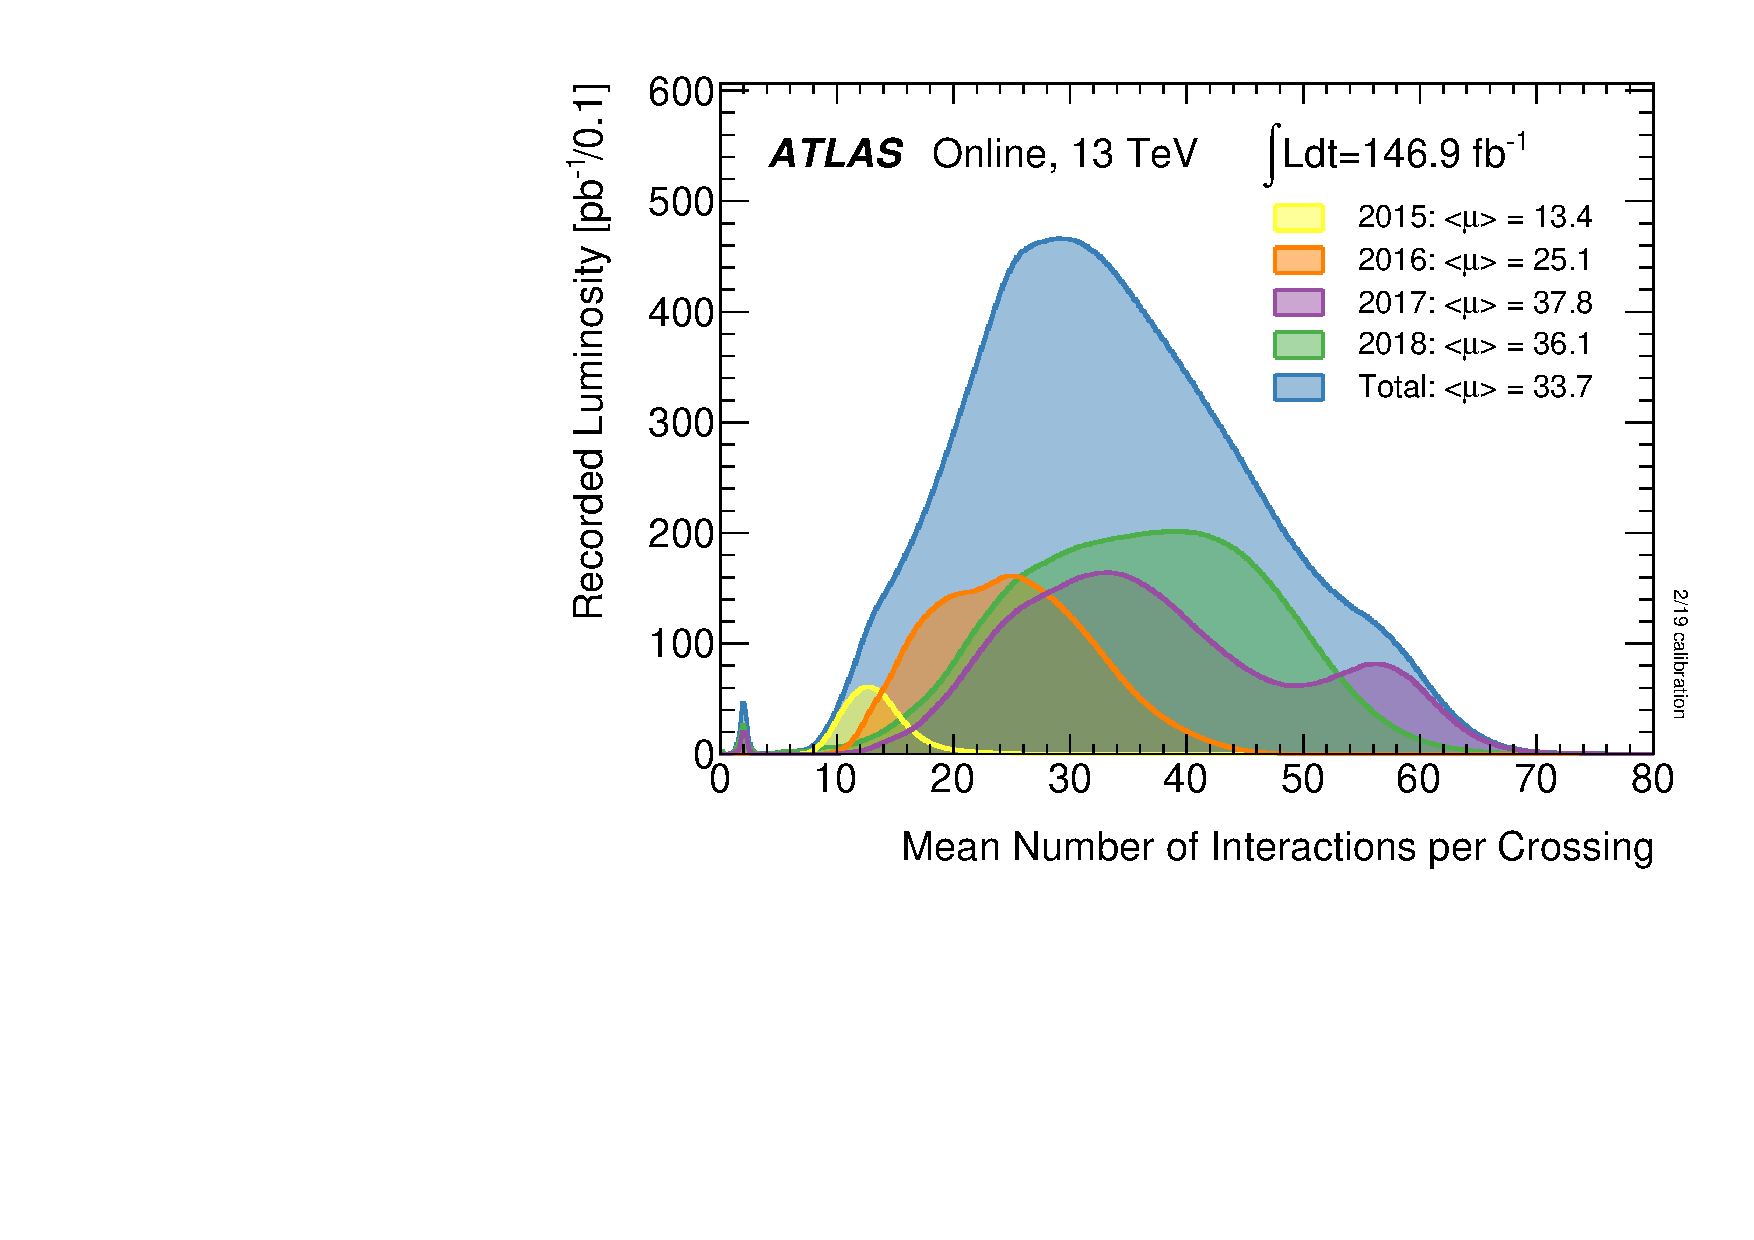
\includegraphics[width=0.8\textwidth]{figures/experiment/pileup}
  \caption[Mean number of interactions per bunch crossing]{ATLAS recorded
  integrated luminosity as a function of the mean number
  of interactions per bunch crossing. Years of data-taking
  are shown in distinct colours, with the combined dataset profile in blue.
  From Ref. \cite{pileup}.}
  \label{fig:exp:pileup}
\end{figure}

\section{Detector overview}

The ATLAS detector schematic is shown in Figure \ref{fig:exp:atlas} and
reveals its cylindrical geometry that divides most systems in a coaxial 
tubular ``barrel'' parts, and disc-shaped ``endcap'' parts, providing
a nearly $4\pi$ solid angle coverage.

The ATLAS coordinate system places
the origin at the centre of the detector at the nominal collision point,
points the $x$-axis towards the centre of the ring, the $y$-axis vertically
upwards, and the $z$-axis along the beampipe in the direction that
completes the right-handed coordinate system. The azimuthal angle $\phi$
and polar angle $\theta$ are defined as usual in spherical coordinates.
However, rapidity
\begin{equation}
y = \frac{1}{2}\ln{\left( \frac{E+p_z}{E-p_z}\right)}
\end{equation}
is preferred over $\theta$ as the differences in rapidity are invariant
under Lorentz transformations in the $z$ direction. In the relativistic
limit pseudorapidity
\begin{equation}
\eta = - \ln{\left(\tan{\frac{\theta}{2}}\right)}
\end{equation}
can be used instead \cite{Thomson:2013zua}.

ATLAS magnet system consists of a solenoid just outside the tracker,
which provides a relatively uniform 2 T magnetic field for the
tracker, and a toroidal magnet system outside the calorimeters, which provides
magnetic field for the muon spectrometer.

\begin{figure}[h]
  \centering
  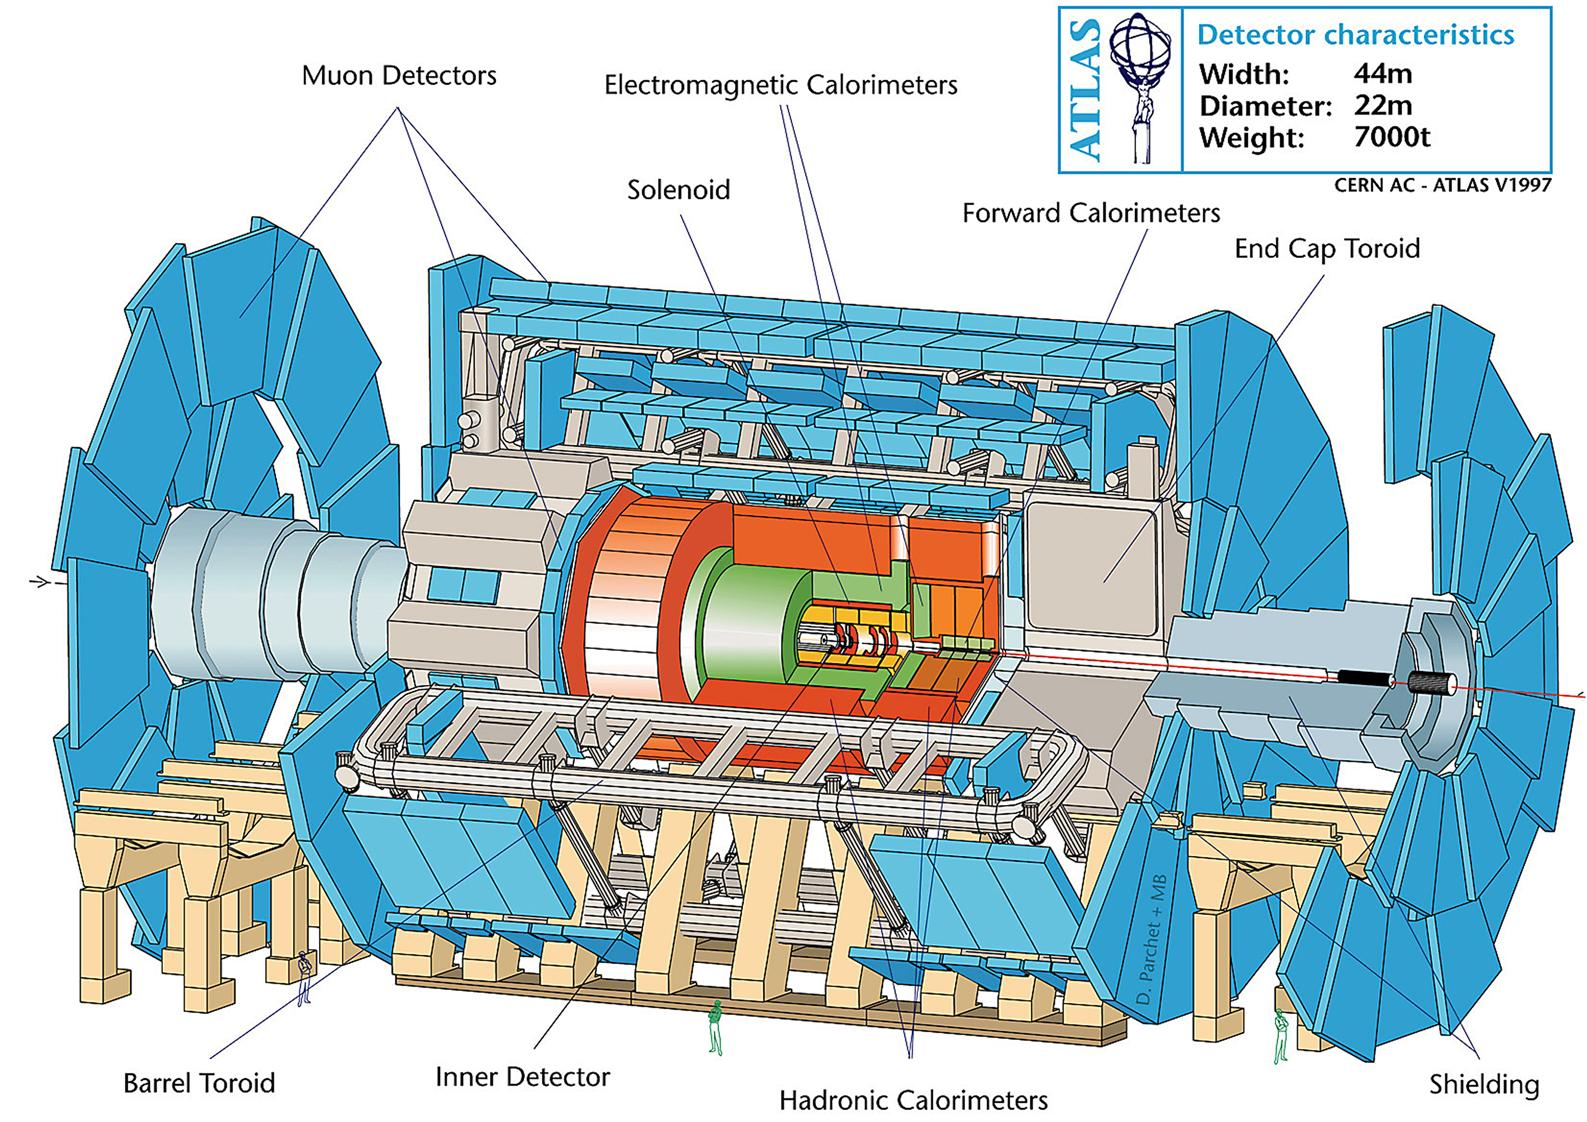
\includegraphics[width=1\textwidth]{figures/experiment/atlas}
  \caption[The ATLAS detector.]{The ATLAS detector schematic. Inner
  detector contains a tracker system and is immersed in a 2 T magnetic field
  provided by the solenoid magnet. Outside the solenoid there is
  an electromagnetic calorimeter, followed by the hadronic calorimeter.
  Finally, in the outermost layer, a muon spectrometer identifies muons
  and measures their curvature in a magnetic field provided by the
  toroidal magnet system.
  From Ref. \cite{Aad:2008zzm}}
   \label{fig:exp:atlas}
\end{figure}

As particles travel outwards from the interaction point they pass a
sequence of detector components. The first is the inner detector,
a silicon and transition radiation tracker which precisely measures the
positions of charged particles at several concentric layers, allowing for
the reconstruction of their trajectories. After passing the solenoid
surrounding the inner detector charged particles and photons deposit
energy in the electromagnetic calorimeter (ECAL), which stops most electrons
and photons. Hadrons are mostly stopped in the hadronic calorimeter
just outside the ECAL. Only muons and neutrinos reach the muon spectrometer
which provides a position measurement of muons allowing for their
identification and a complementary measurement of transverse momentum
\cite{Aad:2008zzm}. A trigger system, described in the next section,
decides whether an event is kept or discarded to reduce the data
rates to a manageable level.

\section{Trigger}

The enormous collision rate and the associated data rate makes it
impossible for the readout system to record every single event. A fast
event filtering is performed by the ATLAS trigger, a two level system
designed to reduce event rates from 40 MHz to a more manageable 1 kHz.

Level-1 trigger is implemented in hardware and reduces the rate of
collisions from 40 MHz to 100 kHz. It works by utilising information
from the calorimeters and the dedicated muon triggers using simple
and fast logic. High-level trigger (HLT) is software-based and further
reduces event rates to 1 kHz, using basic tracking information from both
the tracker and the muon spectrometer.

Events can be selected by the trigger by passing one of the several
requirements, motivated by different physics purposes. These requirements
can be changed in different data-taking periods to balance physics needs
and the changing beam conditions. Some requirements are satisfied too
often and need to be prescaled, keeping only a certain fraction of events
passing the trigger. Un-prescaled triggers keep all of the events that
pass the requirements \cite{Aaboud:2016leb}.

\section{Tracking}

Tracking of particle trajectories near the interaction point is critical
for a number of essential reconstruction tasks, including not only
the measurements of position, charge, and momentum of particle tracks, but also
the ability to associate tracks to vertices, and flavour tagging.

Arguably the most important task of the tracker is to precisely measure
the momentum of the charged particles. The trajectories of charged
particles follow a helical path in an axial magnetic field provided
by the solenoid. Particles passing the tracker layers ionise the active material,
which is digitised and recorded as hits, and finally a fit is performed
to obtain the parameters of the tracks and the associated uncertainties.
The charge of the particle can be determined by the 
sign of the curvature, while the transverse momentum ($\pt$) can be
determined from the curvature of the track
\begin{equation}
\pt = \frac{0.3 B L^2}{8s},
\end{equation}
in the limit where $L \ll R$, where $L$ is the size of the tracker,
$R$ is the radius of curvature of the track, $B$ is the magnetic field
strength, and $s$ is the \textit{sagitta}, the largest distance between
the arc and the chord, perpendicular to the chord \cite{Ragusa:2007zz}.

The tracker is designed to reconstruct tracks with $\pt > 0.5$ \GeV, and
$|\eta| < 2.5$, and comprises several subcomponents, shown in Figure
\ref{fig:exp:tracker}:
\begin{itemize}
\item Pixel detector is the innermost part of the tracker system and
consists of three cylindrical layers of silicon pixel detectors in the
barrel region, and three disks in each of the endcap regions with a total of
approximately 80 million channels. A large number of channels is needed
to prevent occupancy issues in the high track multiplicity environments
and to enable good hit position resolution. Before LHC Run 2 a new layer,
called insertable B-layer (IBL), was added between the beam pipe and the
then innermost pixel layer in order to provide robustness against
inefficiencies in the pixels caused by radiation damage and to improve
momentum resolution. The pixel pitch in the bending plane, relevant for the
measurement of $\pt$, is 50 $\um$ \cite{CERN-LHCC-97-016, Aad:2008zzm, Capeans:1291633}. 
\item SCT, a silicon microstrip detector, is the intermediate subcomponent
of the tracker and consists of four cylindrical layers in the barrel region
and 9 disks in each of the endcaps with a total of approximately 6 million
channels. The strip pitch in the bending plane is 80 $\um$ to maintain
precision in the $\pt$ measurement, while the reduction in the number of
channels is achieved by longer sensors in $z$ direction \cite{CERN-LHCC-97-016, Aad:2008zzm}.
\item TRT, the transition radiation tracker, is the outermost part of the
tracker system. Unlike its silicon counterparts it does not come in layers
but rather a homogenous set of straw drift tubes, as illustrated in
Figure \ref{fig:exp:tracker}. It measures the distance between the track
and the central wire by measuring the time it takes for the ionisation
created by the track to drift to the central wire. The tubes are 4 $\mm$
in diameter, but their resolution in the bending plane for individual
straws is about 130 $\um$, and combined with a large number (typically 36)
of hits per track the TRT provides a meaningful contribution to the
$\pt$ measurement \cite{CERN-LHCC-97-016, Aad:2008zzm}.
\end{itemize}

\begin{figure}[h]
  \centering
  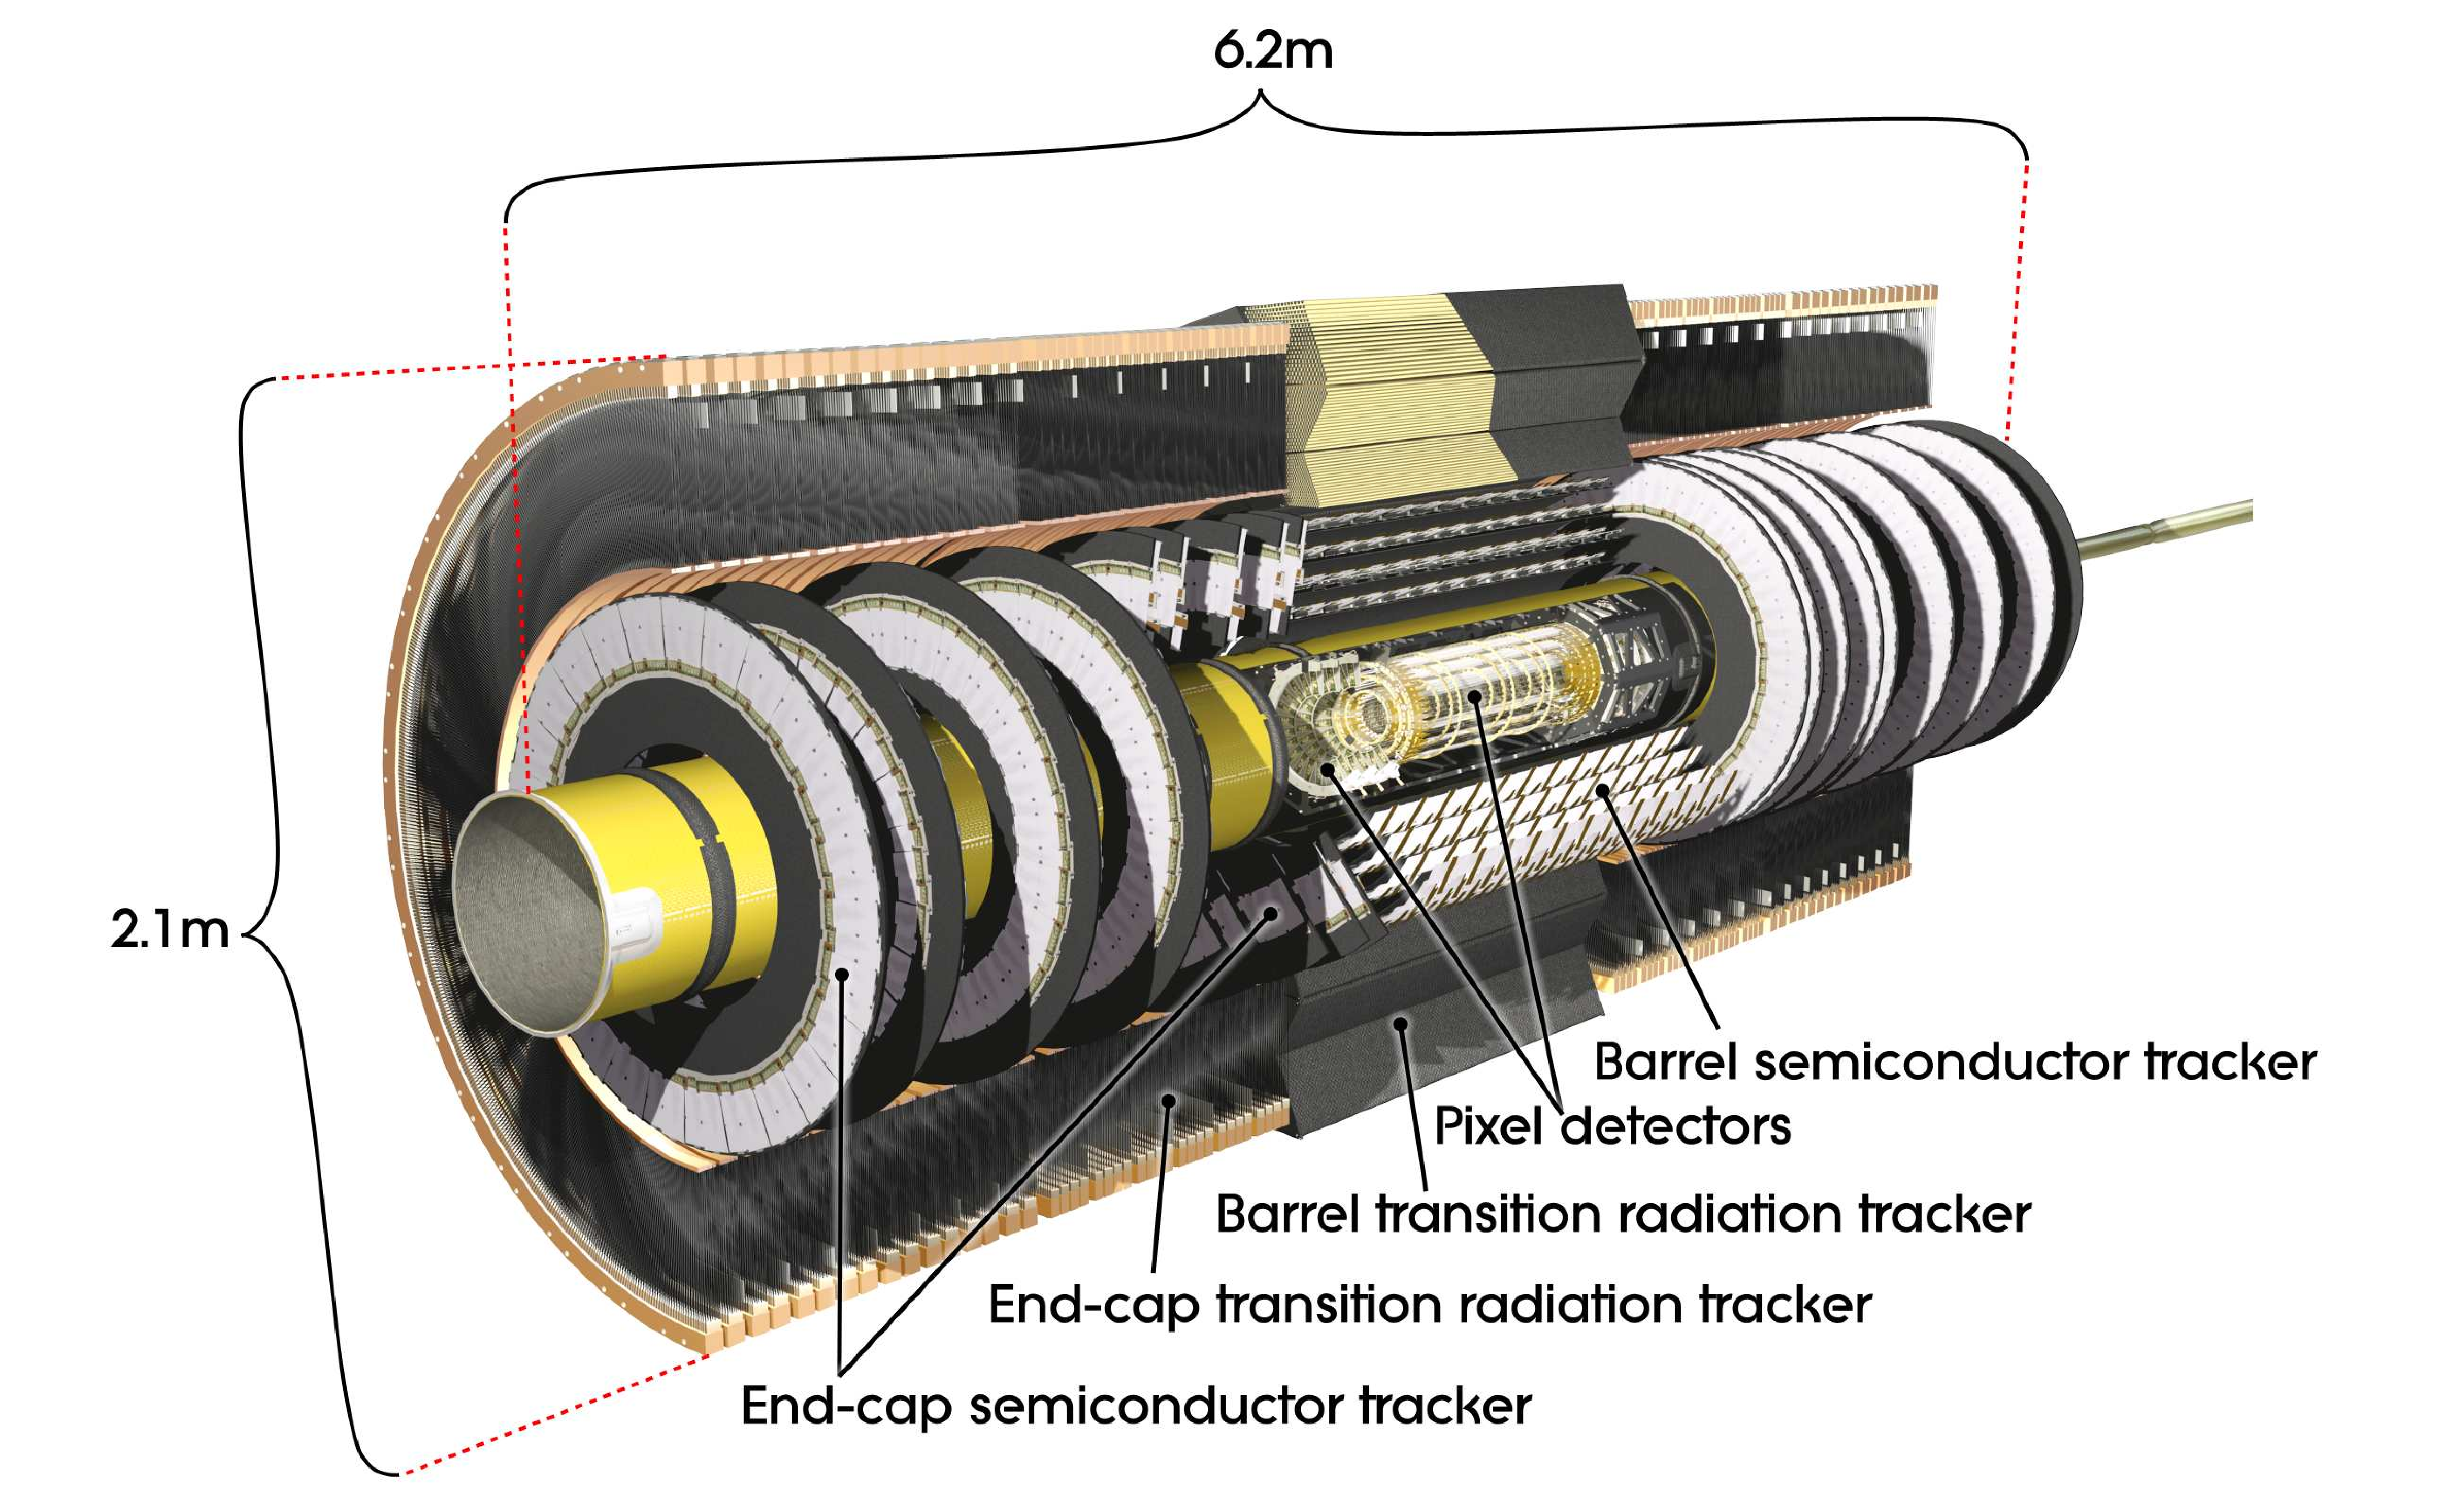
\includegraphics[width=0.8\textwidth]{figures/experiment/tracker}
  \caption[The ATLAS tracker.]{A cross-section of the barrel region
  of the ATLAS tracker system. It consists of the pixel detector,
  the silicon strip detector (SCT), and the transition radiation
  tracker (TRT).
  From Ref. \cite{Potamianos:2016ptf}}
   \label{fig:exp:tracker}
\end{figure}

\section{Calorimetry}

Unlike the tracker, which aims to minimally disrupt the traversing
particles, the calorimeter system is designed to measure the
particle energy by stopping them completely. This ensures a less
noisy measurement of the energy and allows the measurement of
missing transverse momentum.

The calorimeter system provides coverage
up to $|\eta| < 4.9$ with granularity and number of layers varying
throughout the $\eta$ range to satisfy physics requirements. The
components of the calorimeter are sampling rather than homogeneous
type, meaning that it uses alternating layers of a dense material
producing the shower and layers which measure the energy. The
components also share another important characteristic, namely that
the relative energy resolution improves with increasing $\pt$ of
the traversing particle, in contrast with the performance of the
tracker.

Radiation length ($X_0$) of a material is the length that a high
energy electron traverses before its energy decreases to $1/e$ of
its initial energy, primarily via bremsstrahlung and e$^+$e$^-$
pair production. A related quantity for hadrons is the nuclear
interaction length ($\lambda$), defined as the mean distance traversed by a
hadron before an inelastic nuclear interaction. 

While complex geometrically, the calorimeter system can be divided
in two parts based on their physics task:
\begin{itemize}
\item Electromagnetic calorimeter (ECAL) is used for precision
energy measurements of electrons and photons up to $|\eta| < 3.2$.
It is divided in the barrel and endcap parts and uses lead as
the passive material causing the development of electromagnetic
showers, and the liquid argon as the active material. The total
material budget of the ECAL is larger than 22 $X_0$ radiation
lengths in the barrel and larger than 24 $X_0$ in the endcaps 
\cite{CERN-LHCC-96-041, Aad:2008zzm}.
\item Hadronic calorimeter (HCAL), used for energy measurements
of hadronic showers and containment of neutral particles, extends
up to $|\eta| < 4.9$ and provides approximately 11 interaction
lengths ($\lambda$) of hadronic depth. The hadronic endcap
calorimeter and the forward calorimeter both work with liquid
argon as the active material, while the tile calorimeter in the
barrel uses steel as the absorbing material and scintillating
plastic tiles as the active material \cite{CERN-LHCC-96-041,
artamonov2008atlas, Aad:2008zzm}.
\end{itemize}

\section{Muon spectrometry}

Muon spectrometer is the outermost part of ATLAS and was designed to
trigger on muons up to $|\eta| < 2.4$ and measure their transverse momentum up
to $|\eta| < 2.7$. It works by measuring the sagitta of the tracks
in a magnetic field, similarly to the tracker. However, the field
bends muon tracks in the $y-z$ plane, and is provided by three sets of
toroidal magnets, one in the barrel, and one in each of the endcaps,
as shown in Figure \ref{fig:exp:atlas}. 

\begin{figure}[h]
  \centering
  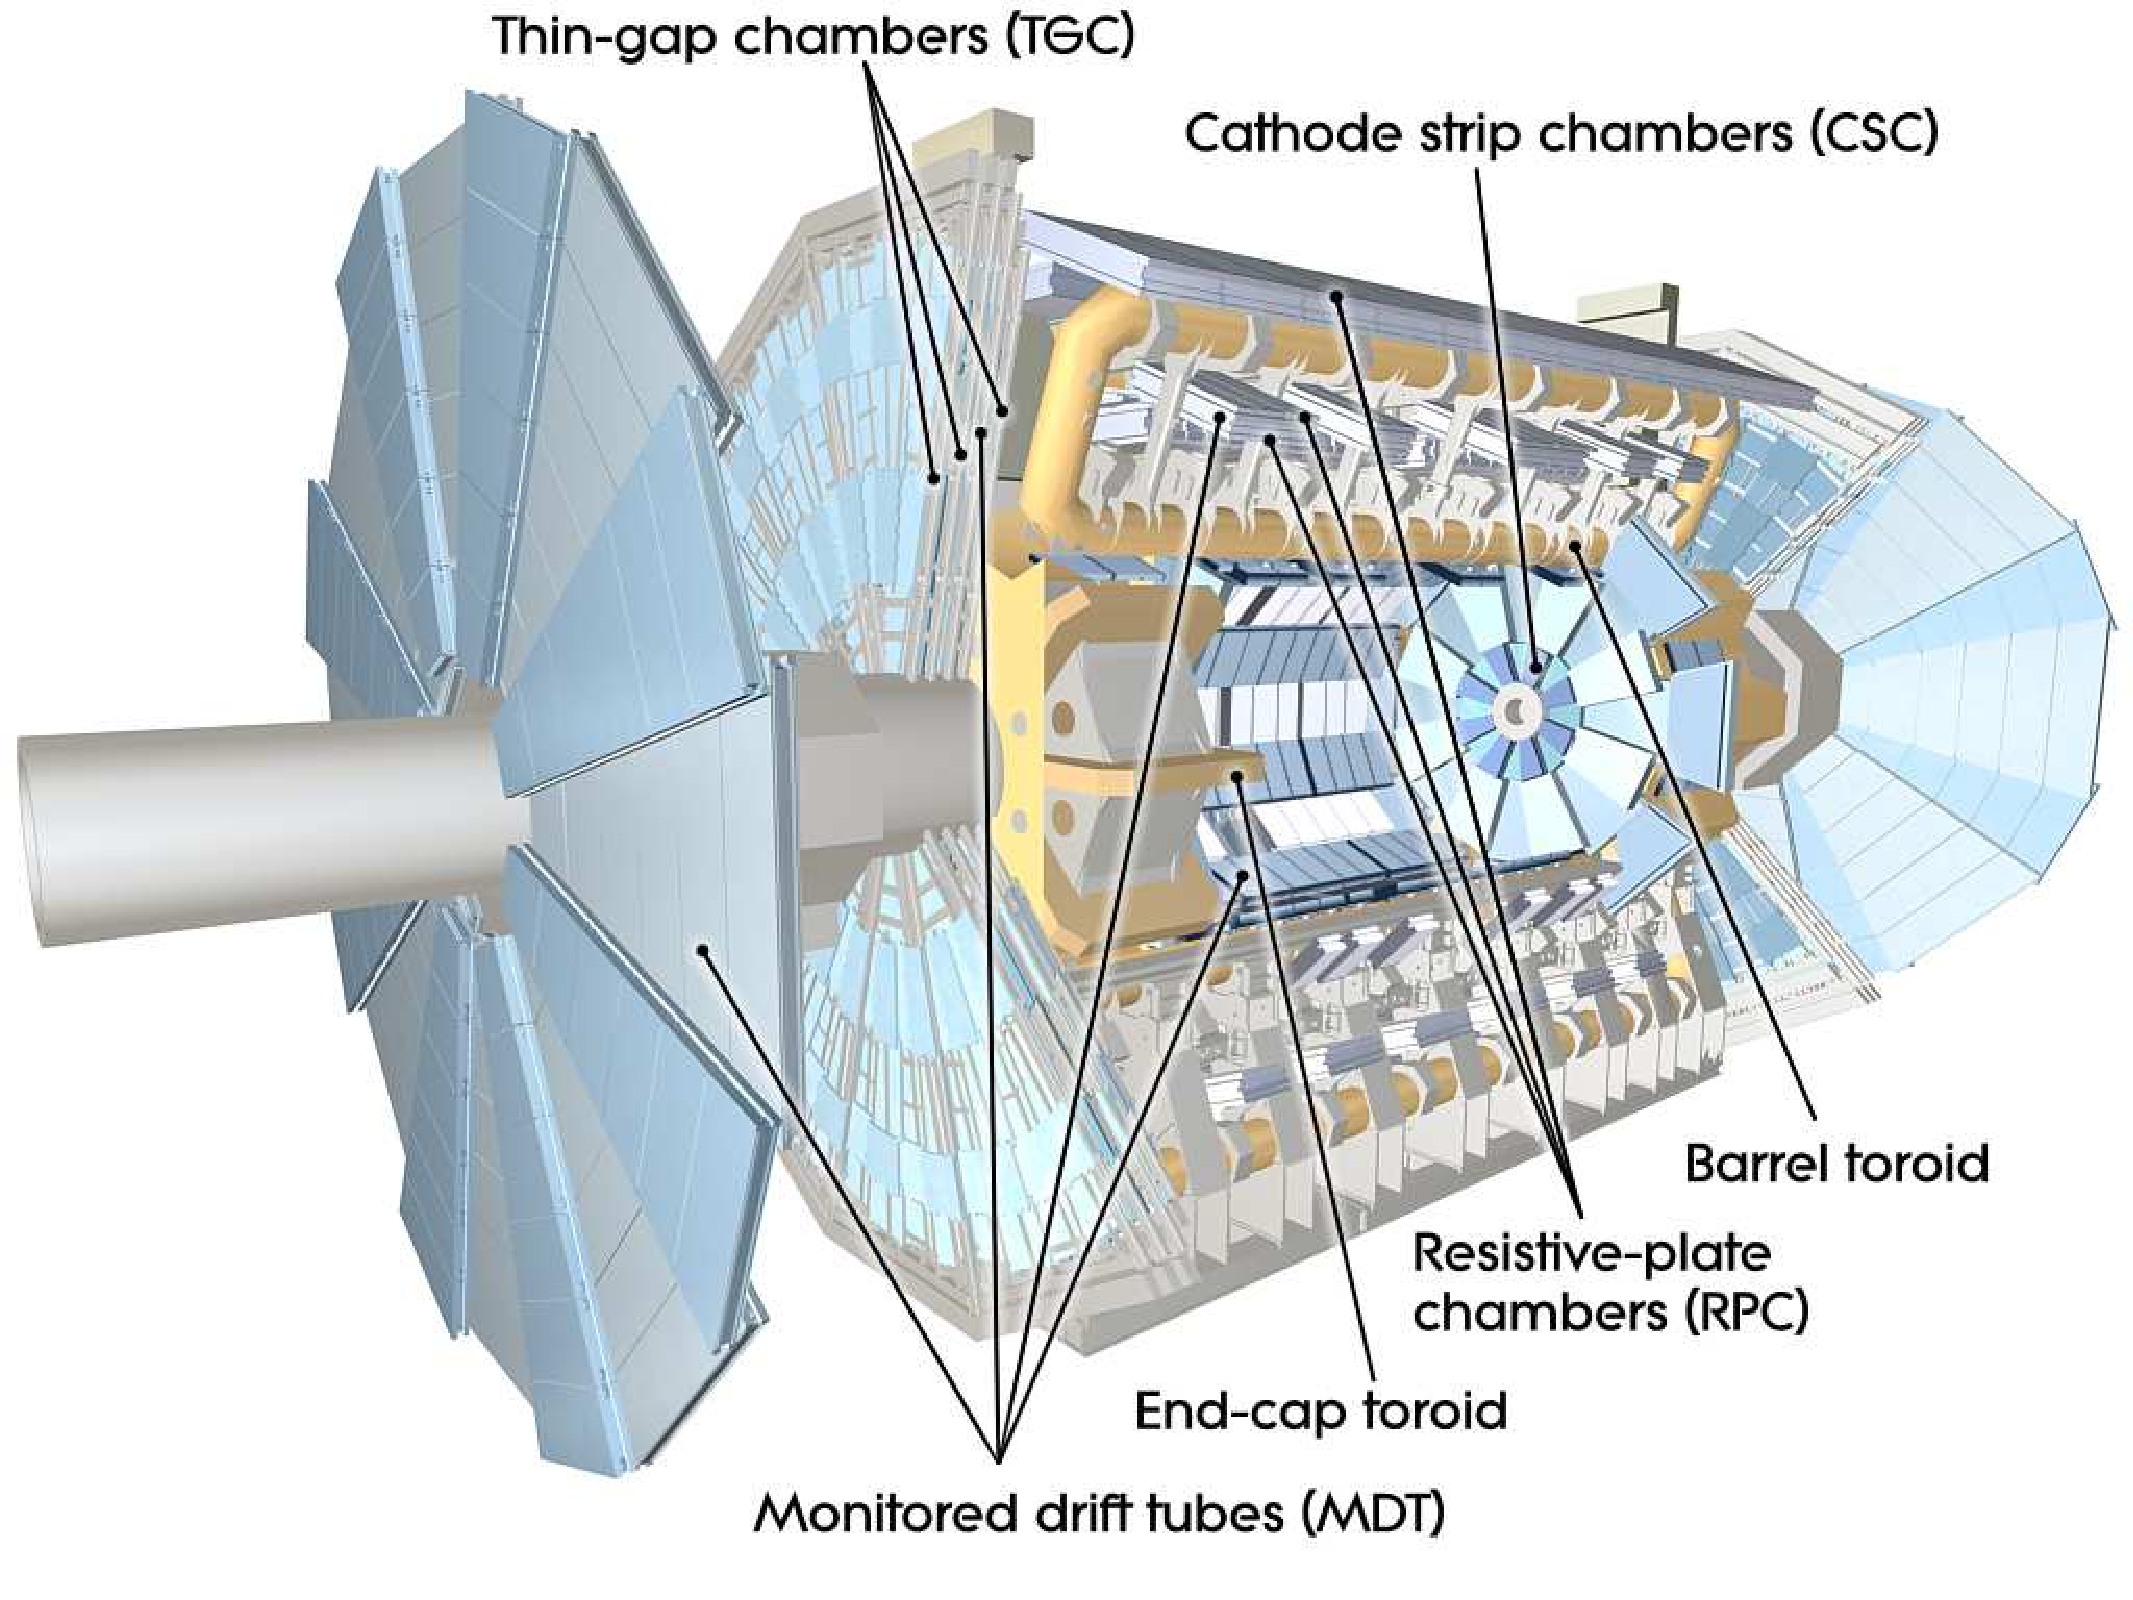
\includegraphics[width=0.8\textwidth]{figures/experiment/muonspectrometer}
  \caption[The ATLAS muon spectrometer.]{Schematic of the ATLAS muon
  spectrometer geometry in the $x-y$ plane in the barrel region. MDT
  chambers, shown in cyan, provide the precision $\pt$ measurement
  capabilities, while the RPC chambers allow triggering. ATLAS support
  structures are shown in yellow.
  From Ref. \cite{Aad:2010ag}}
   \label{fig:exp:ms}
\end{figure}

Monitored drift tube (MDT) chambers provide precision tracking up to
$|\eta| < 2.7$ with the goal of measuring a $\pt = 1$ TeV muon
to 10\% accuracy. The sagitta at this $\pt$ is about 500 $\um$,
meaning that the required accuracy is better than 50 $\um$.
In the barrel, the chambers are arranged in three concentric
layers approximately 5 m, 7.5 m, and 10 m away from the beampipe, as
shown in Figure \ref{fig:exp:ms}. The chambers in the two endcaps are
arranged in wheels perpendicular to the $z$-axis. There is a gap in
the MDTs close to $\eta = 0$ to allow for cabling and services to
the solenoid, calorimeter, and the tracker. Another gap is required
for the detector support structure. The chambers are typically
made of three layers of tubes on each side of the support structure
and achieve a resolution of about 80 $\um$ per tube and about
35 $\um$ per chamber. The relative position of the chambers must also be
known to about 30 $\um$ to achieve the required precision on the sagitta
measurement, which is made possible by a combination of an optical alignment
system and track-based alignment \cite{Aad:2010ag, Aefsky:1380912, Aad:2008zzm}.

% drift time ~ 700 ns, counting rates 30kHz per tube expected at 'full LHC lumi'
% which gives 30us to each if equally spaced arrivals

Cathode strip chambers (CSC) are multiwire proportional chambers
used in the very forward region ($2 < |\eta| < 2.7$)
in the innermost layer in the two endcaps because of their capability
to deal with a higher rate of collisions and better time resolution
\cite{Aad:2010ag}.

Resistive plate chambers (RPC) are gaseous detectors used for
triggering in the barrel ($|\eta| < 1.05$) due to their good time resolution
and tolerance to high rates \cite{Cattani_2011}. In the endcaps ($1.05 < |\eta| < 2.4$)
thin gap chambers (TGC), operating on the same principle as the multiwire
proportional chambers, are used instead \cite{Nagai:1996mf}.





\chapter{Muons in ATLAS}
  
\textit{I really need to find a quote for this chapter}
\vspace{5mm}
\begin{flushright}
--- Miha Zgubi\v{c}
\end{flushright}

\thispagestyle{empty}
\newpage
The ATLAS detector, described in the previous chapter, is a monument
to the engineers and physicists who designed and built it. However,
in order to turn its raw output of nearly one hundred million readout
channels per event to physics knowledge, it requires an intermediate step:
the reconstruction of physics objects.

Muons, the central physics object in this thesis, are reconstructed
by combining the information from the tracker and the muon spectrometer.
In order to be able to do precision studies the Monte Carlo (MC)
simulation of the detector response needs to be calibrated to match
the response in the real detector. In particular, the transverse momentum of
muons needs to be calibrated to the resolution obtained in the real
detector. Similarly, the reconstruction, track-to-vertex-association (TTVA),
and isolation efficiencies need to be calibrated to match those in 
recorded data. These calibrations are obtained through measurements
and carry associated uncertainties.

This chapter describes the first novel contributions from the author.
The first is an improved method of background subtraction in the isolation
efficiency measurements, which significantly reduces the systematic
uncertainty for muons with $\pt < 15$ \GeV. The second is an attempt
to improve muon momentum resolution.

\section{Reconstruction}

Tracks in the inner detector are reconstructed indiscriminately for
all charged particles. First, raw data from the detectors is converted
into space-points which form the basis of tracking. The main track finding
algorithm proceeds inside-out by finding the seeds in the silicon layers.
The seeds are then combined into roads and the extension to the TRT layer
is probed to add hits in the outermost layer. The final collection of hits
is fit to obtain the track parameters \cite{ATLAS-CONF-2010-072, Cornelissen:1020106}.
Tracks with at least $\pt > 400$ \MeV~and some other requirements, found
in Ref. \cite{ATL-PHYS-PUB-2015-026} are then used to find the primary
vertices. The reconstruction of primary vertices proceeds by first finding
the vertices and then fitting them \cite{Aaboud:2016rmg}. Finally, tracks
are associated with vertices which allows the computation of $d_0$, the
transverse impact parameter, which quantifies the shortest distance
between the track and the beam-line, and $z_0$, the longitudinal impact
parameter, which quantifies the difference between the $z$ coordinate
of the associated primary vertex, and the $z$ coordinate of the point
where $d_0$ is computed.


Muon reco in MS, combination.

Muon reconstruction algorithms, muon types.

\cite{ILLINGWORTH198887} % hough transform

Efficiencies, scale factors, tag and probe method.
\cite{Aad:2016jkr} % muons

\section{Momentum calibration}

Things that affect the resolution.

\section{Isolation}

\section{Isolation background subtraction}

\section{VADER4mu}

\section{Other objects}

\chapter{Search for the $\hmumu$ decay}

\textit{"The Higgs boson may, or may not, couple to the second generation fermions."}

\vspace{5mm}
\begin{flushright}
--- a bright bunch of ATLAS scientists.
\end{flushright}

\thispagestyle{empty}
\newpage

The interactions between the Higgs boson and the vector bosons and
third generation fermions, critical to the discovery in 2012, soon 
became the preferred way to study the properties of the Higgs boson.
The mass \cite{Aad:2015zhl, Aaboud:2018wps, CMS-PAS-HIG-19-004},
as well as inclusive and differential cross-sections
\cite{Aad_2015, Chatrchyan_2014, Aaboud:2017oem, Sirunyan:2018sgc, Aaboud:2018ezd},
have been measured and new production modes, $\tth$ \cite{Sirunyan:2018hoz, Aaboud:2018urx}
and $\vh$ \cite{Sirunyan:2018kst, Aaboud:2018zhk}, have been 
observed. However, the interactions between the Higgs boson
and the first or second generation of fermions have not been
observed yet due to experimental challenges. In the leptonic
sector the main challenge is a very small branching fraction due
to the small mass of electron and the muon compared to the tau.
In the quark sector some branching ratios, for example to the charm
quark pair, are larger than those in which the Higgs was discovered.
However, detection is experimentally difficult in the LHC environment
due to the difficulty in flavour tagging, and estimating and modelling
backgrounds \cite{Aaboud:2018fhh, CMS-PAS-HIG-18-031}. Ultimately the
decay to muon pairs offers the best sensitivity to probe the
interactions between the Higgs boson and the second generation
fermions.

In the Standard Model the branching ratio of the Higgs boson with a
mass of 125.09 \GeV~is predicted to be $2.17 \times 10^{-4}$
\cite{deFlorian:2016spz}. This could be modified by physics beyond the
SM \cite{Giudice:2008uua, Dery:2013rta, PhysRevD.80.095023}, meaning
that any deviation from the predicted value could be a sign of new
physics.

ATLAS and CMS experiments have already conducted searches using
the LHC Run 1 data collected at centre-of-mass energies $\sqrts = 7$
and 8 \TeV, both setting the 95\% confidence level upper limits on the
product of the Higgs production cross-section and the branching ratio
to muon pairs \cite{Aad:2014xva, Khachatryan:2014aep} of about seven
times the SM expectation. Using the data collected at $\sqrts = 13$
\TeV, in years 2015 and 2016 the observed upper limit was further
decreased to 2.8 and 2.9 by ATLAS and CMS respectively
\cite{Aaboud:2017ojs, CMS-PAS-HIG-17-019}, with ATLAS
further updating its result to 2.1 using the data collected in 2017
\cite{ATLAS-CONF-2018-026}. This corresponds to $0.9 \sigma$ expected
significance, meaning that the channel is on the verge of evidence.

This chapter presents the search for the Higgs boson decay to muon
pairs using full ATLAS Run 2 dataset collected between 2015 and 2018
at $\sqrts = 13$ \TeV, almost doubling the integrated luminosity of
the dataset since the last result to $139~\ifb$. The Higgs boson mass
is assumed to be 125.09 \GeV~for all presented results.

The overall strategy of the analysis is to select events with
two oppositely charged muons passing the single muon triggers,
and apply additional requirements
to reduce $\ttbar$ and diboson backgrounds. Events are then split
in three channels based on whether they contain zero, one, or two or
more jets in addition to the muon pair. They are further split in
individual categories using a multivariate discriminant, based
on the differences in kinematics between the muon pairs coming
from a Higgs boson produced in the main production modes, and the
muon pairs coming from background events, which are dominated by
the Drell-Yan spectrum. Signal events tend to be more central and
have higher transverse momentum, their jet multiplicity is higher,
and the VBF production mode has a unique signature of two 
back-to-back high-$\pt$ jets with little hadronic activity between
them. Finally, a maximum likelihood fit to the dimuon invariant mass
spectrum is performed in all categories simultaneously, extracting
the signal strength parameter. The analysis is limited by
statistical uncertainty arising from a limited size of the dataset.
The systematic uncertainties are dominated by the uncertainty on
the background modelling, assessed using a dedicated simulated sample.
Additional systematic uncertainties arise from the normalisation 
of signal sample and migration between the categories, such as
the uncertainty on the production cross-section and branching ratio
from the theoretical side, and luminosity, muon momentum resolution
and detector calibration from the experimental side.

A number of improvements were introduced with respect to the
previous result. Selection was improved by including additional
muons from the corners of detector acceptance, by improving
the resolution of the invariant mass by recovering the final
state radiation, and by better rejection of \pileup~ jets in the
forward region. The allocation of events in the categories was
improved by employing a fully multivariate approach in lieu
of a hybrid approach combining a multivariate discriminant and 
cut-based categories. Finally, the background modelling was
improved by using a new functional form and larger DY simulation
dataset. The total effect of all improvements is an approximately
20--30\% increase in the analysis sensitivity and is dominated
by the improvements from using a fully multivariate categorisation
approach.

\section{Data and MC simulation samples}

The proton-proton collision data used in this analysis was
collected in 2015, 2016, 2017, and 2018 at the centre-of-mass
energy of 13 \TeV~in the main physics stream. It corresponds
to an integrated luminosity of 139 $\ifb$ after passing the data
quality checks which ensure that the important parts of the
detector are switched on and function as intended.

The MC simulation samples are used in the analysis for a 
variety of purposes. The signal samples are used to optimise
the event selection and to determine the normalisation and
shape of the signal model in the analysis categories.
Centrally produced background MC simulation samples are used
to optimise the event selection and to validate the muon
momentum resolution in the analysis categories, but not to
determine the normalisation or shape of the backgrounds.
While the normalisation and shape parameters are determined
in the final fit to data, the functional form is selected
in each analysis category independently using a custom
high-statistics MC simulation of Drell-Yan events.

\subsection{Background samples}

\label{sec:bkg-mc}

The leading irreducible background for the analysis is the
Drell-Yan (DY) production of muon pairs. It is simulated using
\textsc{Sherpa} 2.2.1 with the NNPDF3.0 set of parton
distribution functions (PDF) \cite{Ball:2014uwa} in slices of
$\HT$ and with $c$- and $b$-quark filters, simulating 0--2
jet events at next-to-leading order (NLO) and at leading order
(LO) for 3 and 4 jets using \textsc{Comix} \cite{Gleisberg:2008fv}
and \textsc{OpenLoops} \cite{Cascioli:2011va, Denner:2016kdg}
libraries. Matching with the \textsc{Sherpa} parton showering
\cite{Schumann:2007mg} is done using the MEPS@NLO prescription
\cite{Catani:2001cc, Hoeche:2012yf, Hoeche:2011fd}.
In order to populate the tails of the
DY invariant mass distribution relevant for the analysis an
additional high-statistics sample is generated with identical
setup an an additional cut of $\mmumu > 100$ \GeV. Finally, 
\textsc{Sherpa} is also used to model the electroweak $Z$+jets
process with up to two additional jets at LO accuracy beyond
the first two jets.

With the mass of the top-quark set to $m_t = 172.5$ \GeV, the
$\ttbar$ and single-top samples are generated using
\textsc{Powheg-Box} \cite{powheg, Frixione_2007, Alioli_2010}
with NNPDF3.0 PDF set and parton showering and hadronisation
done in \textsc{Pythia} 8.186 using the A14 parameter set
\cite{ATL-PHYS-PUB-2014-021}. $\ttbar$ cross-section is
computed to next-to-next-to-leading order (NNLO) in
QCD with next-to-next-to-leading logarithmic
(NNLL) soft gluon terms taken into account. The cross-section
of the single-top is computed with prescriptions from
\cite{Kidonakis:2011wy, Kidonakis:2010ux}, and all the processes
($t$-channel, $s$-channel, and $Wt$-channel) are generated
separately.

Diboson processes, $WZ$ and $ZZ$, are generated using
\textsc{Sherpa} 2.2.1 with the NNPDF3.0 PDF set, and are normalised
directly to the \textsc{Sherpa} prediction. Only semi-leptonic
and fully-leptonic decays are simulated.

\subsection{Signal samples}

The largest contribution comes from the $\ggf$ signal sample,
generated with \textsc{Powheg-Box} with PDF4LHC15 PDF set
to next-to-next-to-leading order accuracy with parton shower matching
(NNLOPS) \cite{Hamilton:2013fea}, achieving NNLO in QCD after
the re-weighting in rapidity of the Higgs boson. The cross-section
for the $\ggf$ production mode are computed to
next-to-next-to-next-to-leading order (N3LO) \cite{Anastasiou:2016cez}
in QCD with NLO electroweak corrections applied
\cite{Aglietti:2004nj, Actis:2008ug} under the assumption that
they factorise. \textsc{Pythia} 8 with the AZNLO parameters
\cite{Aad:2014xaa} is used to simulate the decay
of the Higgs boson, final state photon radiation, parton
showering, and hadronisation. 

$\vbf$ and $q\bar{q}/qg \rightarrow \vh$ production modes are
generated to NLO accuracy in QCD using \textsc{Powheg-Box},
while the $gg \rightarrow ZH$ is generated to LO accuracy. Same
PDF set and \textsc{Pythia} tunes are used as in the $\ggf$
generation. VBF cross-section is computed with full NLO QCD
and electroweak corrections \cite{Ciccolini:2007jr, Ciccolini:2007ec,
Arnold:2008rz}, and approximate but highly accurate NNLO QCD
corrections \cite{Bolzoni:2010xr}. VH cross-section is computed at
NNLO in QCD \cite{Brein:2003wg} with NLO eletroweak
corrections \cite{Ciccolini:2003jy}, apart from the
$gg \rightarrow ZH$ which is computed to NLO and next-to-leading-logarithm
accuracy in QCD \cite{Ciccolini:2003jy, Brein:2003wg, Brein:2011vx,
Altenkamp:2012sx, Denner:2014cla, Brein:2012ne, Harlander:2014wda,
Harlander:2018yio}.

$\tth$ production mode is generated using \textsc{MadGraph5\_aMC@NLO}
\cite{Alwall:2014hca, Artoisenet:2012st} at NLO accuracy using
NNPDF3.0NLO PDF set and the A14 tune. The cross-section is
computed to NLO in QCD with NLO electroweak corrections
\cite{Yu:2014cka, Beenakker:2002nc}.

\textsc{Pythia} is also used to
overlay minimum bias events to model the effects of \pileup~for all
simulated events using the NNPDF2.3LO PDF set \cite{Ball:2012cx}
with the A3 parameters \cite{ATL-PHYS-PUB-2016-017}. All signal
and background samples are passed through the full ATLAS
detector simulation. Pile-up re-weighting, object momentum
smearing, and efficiency scale factors are applied to the MC
simulation samples in order to make them mimic the collected data.

\subsection{Custom Drell-Yan sample}
\label{sec:hmumu:customDY}

Extract the signal strength paramater relies on a
maximum likelihood fit to the invariant mass spectrum in data,
using parametrised models of both signal and background. The choice
of the functional form describing the background is crucial because
a mismodelling of the background results in a bias on the extracted
signal strength. This is particularly significant when the
signal-to-background ratio is very small, because the impact can be
large.

In order to select the functional form and evaluate the resulting
bias, referred to as the ``spurious signal", a fit to the
background-only spectrum is performed. Ideally, this would be done
on the background MC simulation described in Section \ref{sec:bkg-mc},
but because of the high computational cost associated with the 
simulation of the detector response the statistics of the sample
are on the same order of magnitude as the data. As a result, the
the extracted spurious signal value is unreliable and dominated by
the statistical fluctuations. A custom high-statistics sample of DY
events is generated to overcome this challenge.

The custom DY sample needs to have significantly larger statistics
than the data, requiring a much faster generation. To facilitate
this, the sample is produced at a generator-level only, skipping
the simulation of showering, hadronisation, and detector response,
replacing them by parametrised smearing functions. The effect on
the dimuon invariant mass spectrum is minimal, and because of the
parametrised smearing the jet mismodelling is a second order effect.
On the other hand, final state radiation (FSR) does have an effect on
the invariant mass spectrum and is simulated by \textsc{Photos++}
\cite{Golonka:2006tw}. This setup was fast enough to generate 20
billion events corresponding to approximately 100 $\iab$ in the 
regions of parameter space relevant for the analysis. A drawback of
the sample is that it only models the dominant DY part of the
invariant mass spectrum.

At generator level, the samples are produced separately for zero
or one parton and two partons in addition to the muon pair:
\begin{itemize}
\item \textsc{Powheg} is used to generate an inclusive NLO $\zmumu$
sample, modelling zero and one parton in addition to the muon pair.
For efficiency reasons two sub-samples are generated, one with
$60 < \mmumu < 95$ \GeV~($2.5\times10^{9}$ events), and the other
with $\mmumu > 95$ \GeV~($10\times10^{9}$ events) requirement. Even
after detector smearing the latter sample dominates the fit region.
\item \textsc{Alpgen} \cite{Mangano:2002ea} is used to generate
events with two partons in addition to the muon pair at LO. The 
computation uses only the matrix element with two additional
partons and requires both of them to have $\pt > 25$ \GeV~as well
as $\Delta R(j,j) > 0.4$ to minimise the overlap with the
\textsc{Powheg} sample. Similarly to the \textsc{Powheg} sample,
events are generated with $60 < \mmumu < 95$ \GeV~($1.75\times10^{9}$
events) and $\mmumu > 95$ \GeV~($2.5\times10^{9}$ events)
requirements. These events are crucial to populate the analysis
categories with a large fraction of the signal events coming from
the VBF production mode.
\end{itemize}
Both samples are corrected in the same way to model the effects of
the detector. Muon momentum smearing is done using parametrised functions
derived from MC simulation described in Section \ref{sec:bkg-mc}.
Effects from identification, reconstruction, isolation, and impact
parameter efficiencies are also derived from MC simulation and 
applied as weights, while trigger efficiency weights are derived
from data. FSR momentum is smeared using parametrised prescription
from the ATLAS subgroup specialising in electrons and photons.
Photons are dropped randomly to emulate the reconstruction
efficiency. Smearing of jet momenta is performed using the parametrisation
from the ATLAS subgroup specialising in jets and missing energy.
The effect of \pileup~jets is modelled by building a library of
jets from minimum-bias events in MC simulation and overlaying a
number of sampled jets from the library for each event. A dedicated
missing transverse energy ($\met$) smearing is derived from the Run 2 data.

\section{Physics objects}

The search for a narrow resonance on top of a smoothly falling
background appears at first sight to require not much more than an
excellent understanding of muons in ATLAS. While the intirety of Chapter
\ref{sec:muons} is dedicated to their performance, the sophistication
of the analysis requires understanding of other objects as well.
Photons are used to recover the final state radiation in order to improve
the resolution of the invariant mass spectrum. Jets are used
as a handle to select events produced in the VBF production mode
and to improve separation from the other backgrounds. Even electrons
are reconstructed, albeit solely in order to reject fake jets. Finally,
missing transverse energy is used to supress top and diboson
backgrounds.

\subsection{Muons}

Muon reconstruction, identification, and isolation are described in
detail in Chapter \ref{sec:muons}. Table \ref{tab:hmumu:muons}
summarises the selection used for the $\hmumu$ analysis.
\begin{table}[h]
\centering
\caption{Summary of the muon selection requirements.}
\label{tab:hmumu:muons}
\begin{tabular}{c c}
\toprule
\midrule
ID selection & Loose \\
\midrule
Isolation selection & FixedCutPflowLoose \\ 
\midrule
$\pt$  & $\pt > 15$ \GeV \\
\midrule
$\eta$ & $|\eta| < 2.7$ \\
\midrule
\multirow{2}{*}{Impact parameters} & $|d_0 / \sigma_{d_0}| < 3.0$ \\
                                   & $|z_0 \cdot \sin{\theta}| < 0.5$ mm\\
\midrule
\bottomrule
\end{tabular}
\end{table}
The majority of reconstructed muons in the Loose selection are
the CB type, combining the information from the tracker and
muon spectrometer systems. However, in order to maximise the
acceptance of signal events other muons types are also used
to improve the reconstruction efficiency in the challenging
parts of the detector. ST and CT improve the reconstruction
efficiency in the $|\eta| < 0.1$ region where the muon
spectrometer has a gap to allow for cabling and services to
the tracker, while the ME muons are used in the forward
regions to reconstruct muons outside of the tracker
coverage, where $2.5 < |\eta| < 2.7$.

CB muons benefit from a combination of two $\pt$ measurements,
the one in the tracker, and the one in the muon spectrometer.
Figure \ref{fig:hmumu:reso} verifies that the resulting dimuon
invariant mass resolution is only marginally worse for muon
pairs containing one non-CB muon (dotted green line) compared
to pairs where both muons are CB (dashed blue line). Since
most muons are CB, the inclusive distribution (solid orange
line) and the distribution of purely CB muons (dashed blue line)
are nearly identical.

The reason for such a small degradation is that the resolution of the combined
$\pt$ measurement is dominated by the tracker $\pt$ measurement
in the barrel region, and by the muon spectrometer measurement
in the forward regions. ST and CT muons, used in the $|\eta| <
0.1$ region, combine a track in the ID with a segment in the
muon spectrometer or with a calorimeter deposit, and thus 
benefit from having the high-quality tracker $\pt$ measurement.
Conversely, ME muons, used in the $2.5 < |\eta| < 2.7$ region,
use the track from the muon spectrometer, the higher quality
measurement in the forward region.
\begin{figure}[h!]
  \centering
  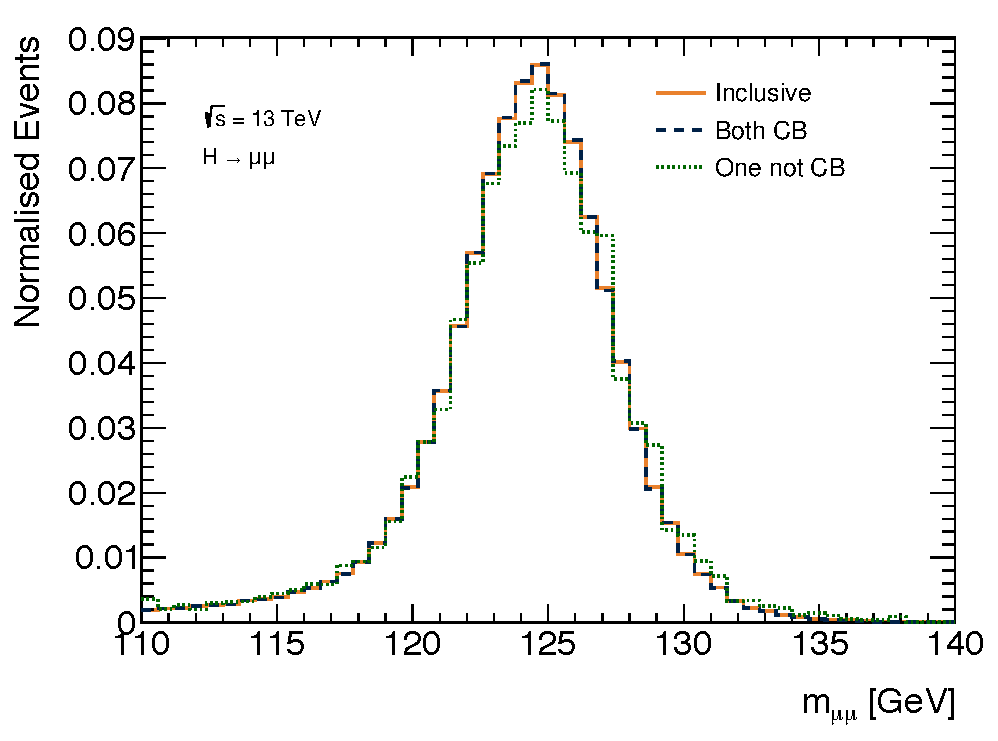
\includegraphics[width=0.8\textwidth]{figures/hmumu/resolution}
  \caption[Muon resolution for different muon types]{Resolution
  of the dimuon invariant mass measurement for the $\ggf$ signal
  sample in the $\hmumu$ analysis signal region. Events in which
  both muons are CB type are shown in dashed blue line, while
  events in which one of the muons is not CB are shown in dotted
  green line. Inclusive distribution is shown in the solid orange
  line.}
  \label{fig:hmumu:reso}
\end{figure}
The FixedCutPflowLoose isolation selection is used because
of a combination of its high efficiency, robustness to high
\pileup~conditions, and an improved rejection of heavy-flavour
jets. The cut on the $\pt$ rejects muons from the decay of
heavy-flavour quarks, while cosmic rays are rejected by the
standard requirements on the impact parameters.

\subsection{Photons and FSR}

Photons are reconstructed in ATLAS via its energy deposits
in the eletromagnetic calorimeter. Unlike electrons, photons
are electrically neutral and do not leave tracks in the
tracker, unless they are converted to electron-positron
pairs before reaching the calorimeter. The details on the
reconstruction algorithm and its performance are described
in Ref. \cite{Aaboud:2018yqu}.

Muons may radiate a photon and thus lose energy, meaning that
the invariant mass of the muon pair is no longer equal to the
mass of the mediator. In order to mitigate this effect up to
one final-state photon candidate is added to the mass
calculation, using a procedure similar to the one used in
Ref. \cite{Aad:2014eva}, but optimised for the high-purity
requirements of this analysis. Collinear photons
($\Delta R(\gamma, \mu) < 0.20$) are required to have $\pt$
larger than a linearly increasing threshold, from
$\pt^\gamma > 3$ \GeV~at $\Delta R(\gamma, \mu) = 0$ to
$\pt^\gamma > 8$ \GeV~at $\Delta R(\gamma, \mu) = 0.2$.
Non-collinear photons ($\Delta R(\gamma, \mu) > 0.20$)
are required to have $\pt^\gamma > 8$ \GeV~and tight \cite{Aaboud:2018yqu}
identification requirement for photons. When multiple
photon candidates are found only the one with the highest $\pt$
is included in the invariant mass calculation, with priority
to the collinear photons over non-collinear ones.

Around 5\% of all signal events have at least one FSR candidate,
of which approximately 90\% are the collinear photons.
The distribution of invariant mass for the MC simulation of
$\ggf$ signal events with at least one reconstructed FSR
candidate is shown in Figure \ref{fig:hmumu:fsr}
before and after the recovery of final state radiation.
It can be seen that the mass peak is shifted much closer to
125 \GeV, with the slight overshoot resulting from the fake
FSR candidates coming from pileup. The improvement in the
invariant mass resolution is approximately 3\% inclusively.
A drawback of the FSR recovery is an $\sim 8\%$ increase in the
number of background events in the signal region due to the
migration of events from the $Z$ mass peak.
\begin{figure}[h!]
  \centering
  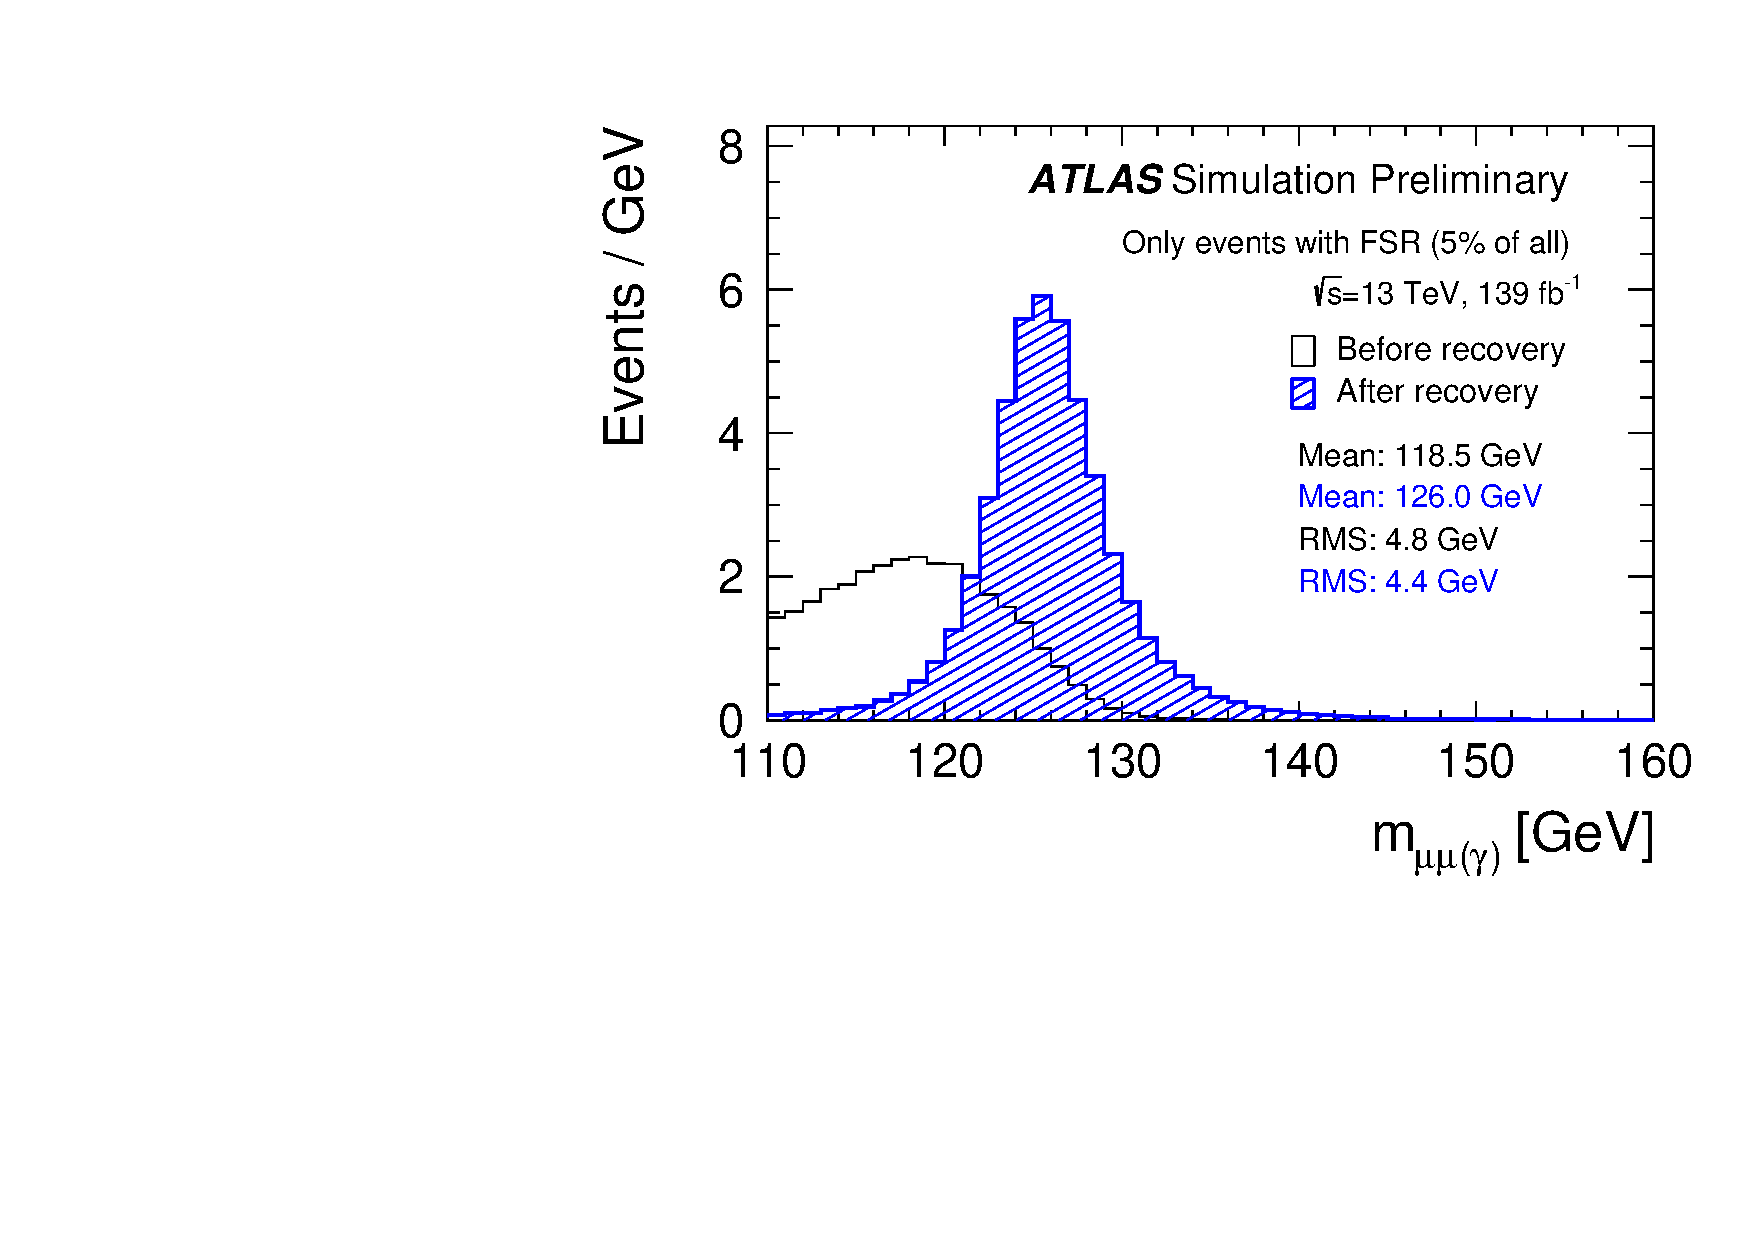
\includegraphics[width=0.8\textwidth]{figures/hmumu/FSR_fsr}
  \caption[Final state radiation recovery]{Invariant mass before
  (white solid) and after (blue hatches) final-state radiation
  recovery for a MC simulation of $\ggf$ signal events passing
  the analysis selection. Only events with one or more
  reconstructed FSR candidates are shown. The mean and the
  root-mean-square of the distributions are shown in the bottom
  right corner. From Ref. \cite{ATLAS-CONF-2019-028}.}
  \label{fig:hmumu:fsr}
\end{figure}

\subsection{Jets, electrons, and $\met$}

Jets are the collimated collections of hadrons, arising either
from a parton in the final state of the interaction, the remnants
of the proton not participating in the hard scatter (underlying event),
or from \pileup~interactions. They are used to identify events
which could have been produced via the VBF production mode by
exploiting its typical dijet signature. Jets are experimentally the richest
objects in ATLAS, reconstructed either from the deposits in the
calorimeters, tracks that the charged hadrons leave in the tracker,
or both. The optimal use of substructure has been extensively
studied both theoretically \cite{Altheimer:2012mn} and using
a wide variety of modern machine learning techniques \cite{Larkoski:2017jix}.
The reconstruction used in this analysis is based on topological
clusters of calorimeter cells \cite{Aad:2016upy}, which are used as
an input to the anti-k$_\text{T}$ clustering algorithm
\cite{Cacciari:2008gp, Cacciari:2011ma} with the distance parameter
$\Delta R = 0.4$. A requirement on the jet $\pt > 25$ \GeV~for the
central jets ($|\eta| < 2.5$), and at $\pt > 25$ \GeV~for the forward
jets ($2.5 < |\eta| < 4.5$).

The suppresion of jets coming from \pileup~ is achieved by using a
dedicated jet vertex tagging (JVT) discrimant \cite{ATLAS-CONF-2014-018},
constructed using tracking information. In the forward region \pileup~
jet suppression is achieved with the fJVT discriminant \cite{Aaboud:2017pou},
using the information on jet shape and the topological correlations in
\pileup interactions.

Jets containing a $b$-hadron are identified using a multivariate
$b$-tagging algorithm \cite{Aaboud:2018xwy} if they are inside the
tracker ($|\eta| < 2.5$). A selection providing 60\% tagging
efficiency for real $b$-jets and less than 0.1\% fake rate for
light-flavoured jets \cite{ATL-PHYS-PUB-2017-013} is used
to tag the jets.
\begin{table}[h]
\centering
\caption{Summary of the jet selection requirements.}
\label{tab:hmumu:jets}
\begin{tabular}{c c}
\toprule
\midrule
Algorithm              & Anti-k$_\text{T}$ ($\Delta R = 0.4$)\\
\midrule
$\eta$                 & $|\eta| < 4.5$ \\
\midrule
\multirow{2}{*}{$\pt$} & $\pt > 25$ \GeV~for $|\eta| < 2.4$ \\
                       & $\pt > 30$ \GeV~for $2.4 < |\eta| < 4.5$ \\
\midrule
\multirow{2}{*}{JVT}   & JVT $> 0.59$ \GeV~for $|\eta| < 2.4$ and $20 < \pt < 120$ \GeV \\
                       & JVT $> 0.11$ \GeV~for $2.4 < |\eta| < 2.5$ and $20 < \pt < 120$ \GeV \\
\midrule
fJVT                   & fJVT $< 0.5$ \GeV~for $2.5 < |\eta| < 4.5$ and $20 < \pt < 120$ \GeV \\
\midrule
b-tag                  & MV2c10 60 WP for $|\eta| < 2.5$ and $\pt>20$ \GeV \\
\midrule
\bottomrule
\end{tabular}
\end{table}
Electrons are reconstructed by matching a track in the ID with a
calorimeter deposit in the ECAL, as described in Ref. \cite{Aad:2014fxa}.
Unlike the topological cluster used for jets, the calorimeter deposits
are clustered using a sliding-window algorithm \cite{Lampl:1099735}
which can be more accurately calibrated due to the fixed size cells.

Electrons are used in the analysis only in the overlap removal
procedure to remove fake jets. The electron selection requirements
are summarised in Table \ref{tab:hmumu:electrons}. Electron candidates
are required to pass the Medium likelihood identification selection
and FCLoose isolation selection \cite{Aad:2014fxa} to
reject electrons from hadronic decays or \pileup. The electron $\pt$
is required to be larger than 7 \GeV, while pseudorapidity has to 
satisfy $|\eta| < 2.47$ with the exception of the crack region
$1.37 < |\eta| < 1.52$. A quality
requirement is used to reject electrons in which a cell is dead 
or faulty, and requirements on the impact parameters are used to
reject electrons coming from heavy flavour decays or other
proton-proton interactions.
\begin{table}[h]
\centering
\caption{Summary of the electron selection requirements.}
\label{tab:hmumu:electrons}
\begin{tabular}{c c}
\toprule
\midrule
Identification & Medium LH \\
\midrule
Isolation      & FCLoose \\
\midrule
$\pt$          & $\pt > 7$ \GeV \\
\midrule
$\eta$         & $|\eta| < 2.47$ excluding $1.37 < |\eta| < 1.52$ \\
\midrule
Quality        & Not "BADCLUSELECTRON" \\
\midrule
\multirow{2}{*}{Impact parameters} & $|d_0/\sigma_{d_0}| < 5$ \\
                                   & $|z_0 \cdot\sin{\theta}| < 0.5$ mm\\
\midrule
\bottomrule
\end{tabular}
\end{table}

Missing transverse energy is defined as the magnitude of the vectorial
sum of $\pt$ of all calibrated muons, electrons, jets, and other tracks
not used in the reconstruction of any objects, referred to as the ``soft
term". The details on the reconstruction algorithm, in particular on the
treatment of the soft term, are available in Ref. \cite{Aaboud:2018tkc},
along with performance studies.

$\met$ can result from neutrinos, which escape the detector without leaving
any deposits, or from experimental inaccuracies when measuring muons,
electrons, or jets. In the analysis $\met$ is used to discriminate between
the signal and $\ttbar$ processes. Instead of a cut is used as
an input to the multivariate discriminant in the 2-jet channel.

A single physical object can create deposits in the detector which are
used by two different reconstruction algorithms to create more than
one particle candidate. For example, an electron results in an ECAL
deposit which is used in both the reconstruction of a jet and an
electron. For this reason an object overlap removal procedure is used
to remove potential duplicates.

Muons are only removed if they are CT type and share a track with an
electron, or they are close to a jet ($\Delta R_{\mu, j} < 0.2$) with more
than two tracks and where muon $\pt$ is less than 0.7 of all track $\pt$.
Jets are removed if they are close ($\Delta R_{e, j} < 0.2$) to
electrons.

\section{Event selection}

A very loose event selection based on oppositely charged muon pairs
is used for the analysis to maximise the number of signal events.
DY background is irreducible, but the $\ttbar$ contributions can be
reduced by a veto on events with a $b$-tagged jets.
The selection, summarised in Table \ref{tab:hmumu:events}, results
in approximately 59\% acceptance for the $\ggf$ and VBF signal events. 
\begin{table}[h]
\centering
\caption{Summary of the event selection requirements.}
\label{tab:hmumu:events}
\begin{tabular}{c c}
\toprule
\midrule
\multirow{3}{*}{Cleaning} &  Pass GRL \\
                          &  Pass single muon trigger \\
                          &  Primary vertex ($> 2$ tracks with $\pt > 0.5$ \GeV)\\
\midrule
\multirow{3}{*}{Muons} & Two oppositely charged muons \\
                       & $\pt^\text{lead} > 27$ \GeV\\
                       & $\pt^\text{sublead} > 15$ \GeV\\
\midrule
Jets                   & Zero $b$-tagged jets \\
\midrule
\bottomrule
\end{tabular}
\end{table}

The ATLAS detector is a complex machine composed of many independent
subcomponents that are being pushed to the limits of their performance.
Failure of detector subcomponents is a normal part of detector operations
and is dealt with by detailed monitoring of performance and the
release of so-called GoodRunList (GRL). The GRL contains a list of 
runs further segmented to two-minute data-taking intervals, called
luminosity blocks, in which the detector operates as intended.
Data used in the analysis is required to be collected in one of those
luminosity blocks in order to veto pathological events.

Furthermore, data is required to pass the lowest unprescaled single
muon triggers, being \texttt{HLT\_mu20\_iloose} or \texttt{HLT\_mu50}
in the 2015 and \texttt{HLT\_mu26\_ivarmedium} or \texttt{HLT\_mu50}
in 2016-2018 data-taking period. These triggers require at least one
isolated muon with a $\pt$ larger than 20 or 26 \GeV~ respectively, or
one non-isolated muon with at least 50 \GeV~\cite{Aad:2014sca}. The increase in trigger
thresholds was required to deal with higher rates of events at an
increased instantaneous luminosity between 2016 and 2018.

Events are required to have at least one reconstructed primary vertex
candidate with at least two tracks with $\pt > 0.5$ \GeV in the inner
detector. When multiple vertices are reconstructed the one with the 
highest scalar sum of $\pt$ of the associated tracks is considered
to be the hard scatter vertex.

Events are required to have exactly two oppositely charged muons.
The leading muon has a $\pt > 27$ \GeV~requirement in order to pass
the trigger thresholds, while the sub-leading muon is required to
have $\pt > 15$ \GeV, with both having a pseudorapidity requirement
of $|\eta| < 2.7$. Additionally, events are required to have zero
$b$-tagged jets to supress $\ttbar$ and diboson backgrounds.

After the common selection the $Z$ control region, the signal region,
and the central and sideband regions are defined by requirements
on the invariant mass, summarised in Table \ref{tab:hmumu:regions}.
\begin{table}[h]
\centering
\caption{Summary of the analysis regions.}
\label{tab:hmumu:regions}
\begin{tabular}{c c}
\toprule
\midrule
$Z$ control region     & $76 < \mmumu < 106$ \GeV \\
\midrule
Fit region             & $110 < \mmumu < 160$ \GeV \\
\midrule
Central region         & $120 < \mmumu < 130$ \GeV \\
\midrule
\multirow{3}{*}{Sideband region} & $110 < \mmumu < 120$ \GeV\\
                                 & or \\
                                 & $130 < \mmumu < 180$ \GeV \\
\midrule
\bottomrule
\end{tabular}
\end{table}

$Z$ control region contains almost one hundred million events
in data and is used to validate detector performance, in
particular to check the muon resolution in data and MC simulation.
The sideband region contains approximately two million events
in the data, which are used to train the multivariate classifier
and to validate the background modelling. The central region
contains appriximately 250,000 events in data, of which about
860 are expected from the SM signal. The final maximum likelihood
fit is performed in the fit region.

The invariant mass spectrum after the recovery of the final
state radiation is shown in Figure \ref{fig:hmumu:sel-mmumu} for data and
MC simulation of signal and background samples for events
passing the selection requirements. The spectrum is dominated by DY
events, especially around the $Z$ mass peak at around 91 \GeV.
The $Z$ peak is also present in the diboson backgrounds, while
the top backgrounds have a smoothly falling spectrum.
Signal events form a narrow peak at around 125 \GeV, with their yields
multiplied by a factor of a hundred for visibility.
\begin{figure}[h!]
  \centering
  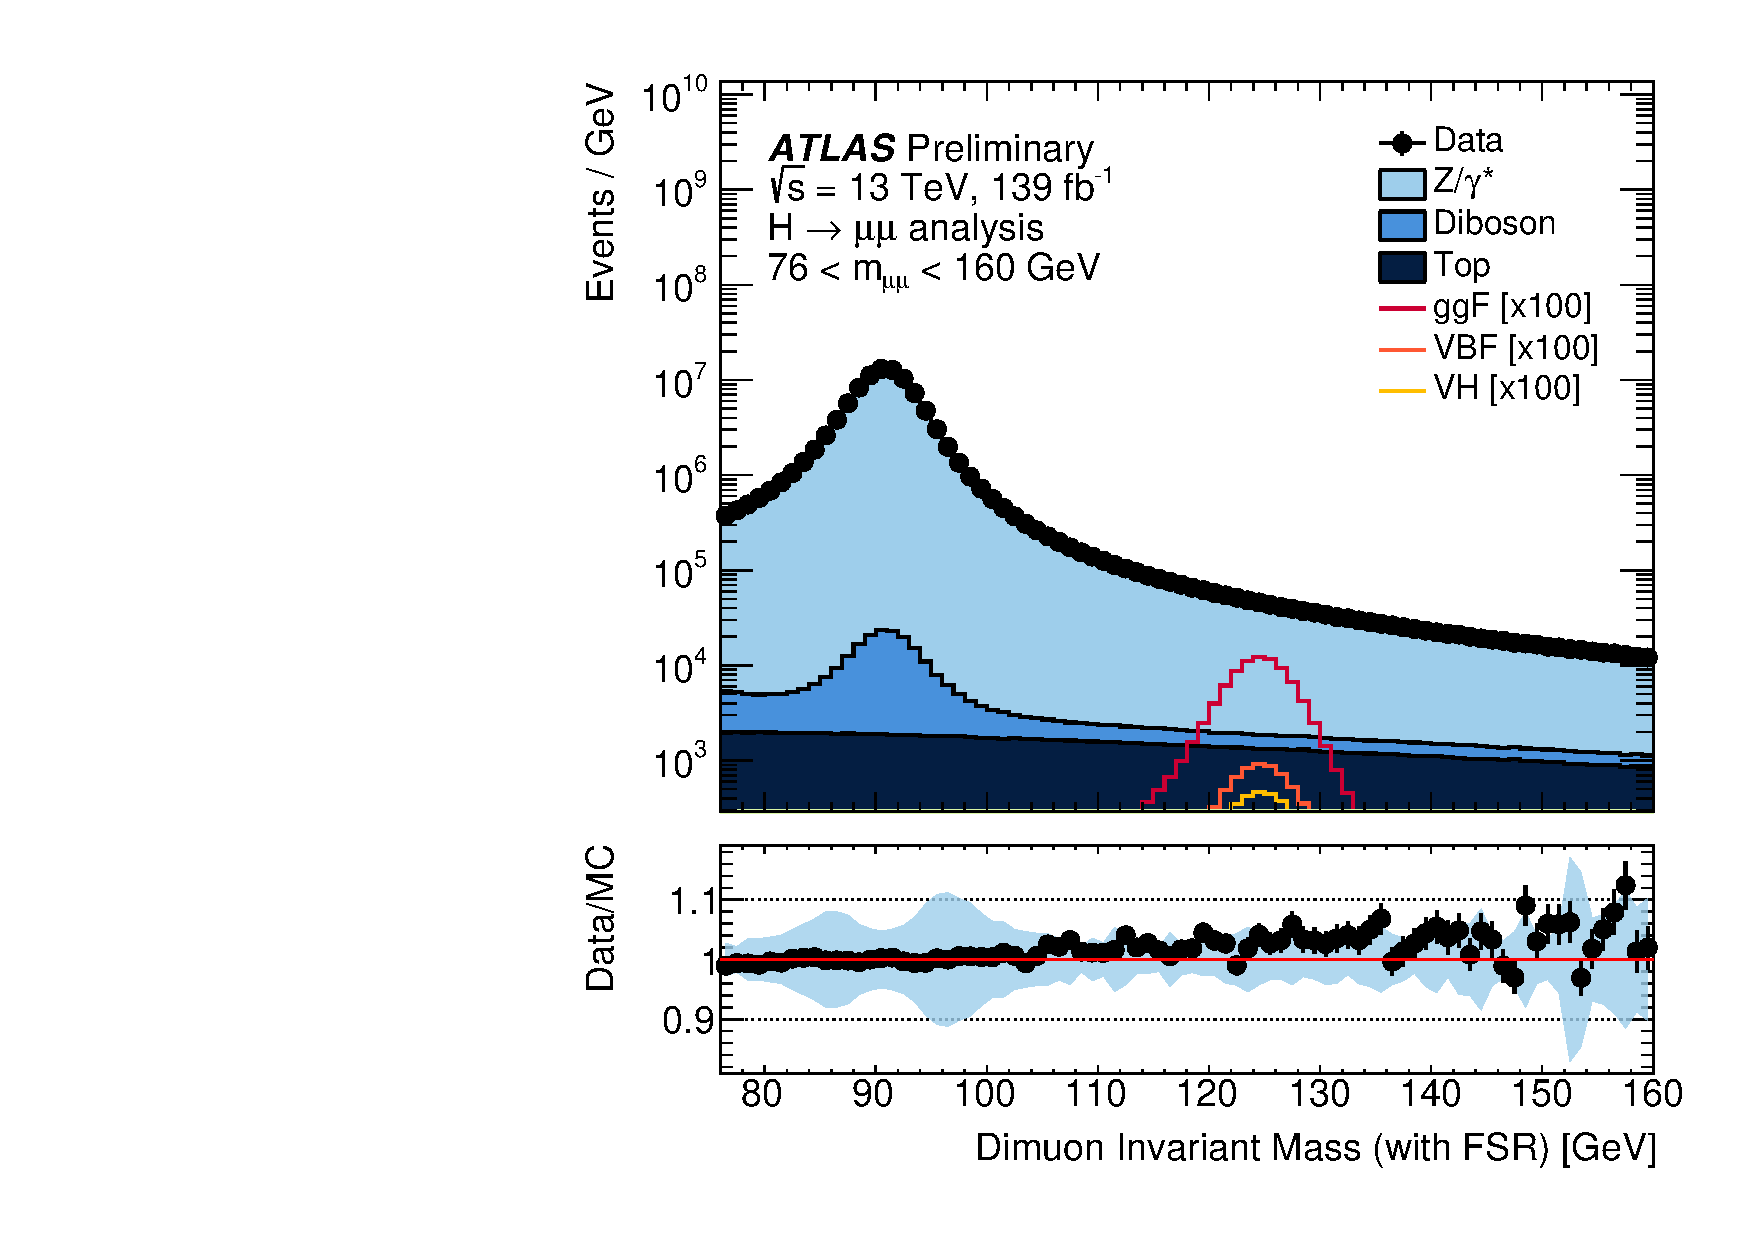
\includegraphics[width=0.9\textwidth]{figures/hmumu/sel-mmumu}
  \caption[Dimuon invariant mass spectrum of selected events.]{
  The invariant mass spectrum after the correction for
  final state radiation, for data corresponding to 139 $\ifb$.
  MC simulation is normalised to the data for easier comparison.
  Data is shown as black markers, the MC simulation of backgrounds
   is dominated by the DY events (light blue),
  followed by diboson (blue) and top (dark blue) contributions.
  Signal events coming from the $\ggf$, VBF, and VH production
  modes are shown as solid red, orange, and yellow lines,
  respectively, with the yields normalised to one hundred times the
  SM prediction for visibility. There are too few $\tth$ events to appear
  on the figure. The bottom panel shows the ratio between the data
  and MC simulation of background events, while the blue band
  represents the experimental systematic uncertainty. Statistical
  uncertainty on both data and MC simulation is combined in the
  error bars on data. From Ref. \cite{ATLAS-CONF-2019-028}}
  \label{fig:hmumu:sel-mmumu}
\end{figure}

\section{Event categorisation}

The goal of event categorisation is to improve the sensitivity of the
analysis by splitting events in categories with different signal
purities. In previous iterations of the analysis physics-based
arguments were used to construct categories targeting the VBF 
production mode and signal enriched regions using requirements on
event kinematics. However, with increased statistics of the
available dataset it became increasingly advantageous to exploit
modern machine learning models and infer the classification scheme
from the available data. With this approach care needs to be taken
to prevent bias and sub-optimal performance due to overfitting.

The categorisation scheme begins by splitting events in categories
based on jet multiplicity: 0-jet, 1-jet, and 2-jet channel, where
the 2-jet channel includes events with more than two jets.
%\footnote{ A categorisation approach without this initial split was tested and
%results in a small ($\sim 1\%$) improvement, but the split was kept
%to minimise systematics from the modelling of jet multiplicity.}
Kinematic differences between signal and background events are
exploited by training boosted decision tree (BDT) classifiers in
each of the jet channels using the XGBoost \cite{Chen:2016:XST:2939672.2939785}
package.

In each of the categories a ``Higgs classifier" is trained to
distinguish between MC simulation of $\ggf$ and VBF events, and the
data events from the sideband region. In the 2-jet
category an additional ``VBF classifier" is trained to distinguish
between the MC simulation of VBF signal events, and the data sidebands.
In both trainings the signal event weights are scaled so that their sum
matches the number of data events. 

The variables used in the training in each of the jet channels are
summarised in Table \ref{tab:hmumu:variables}. 0-jet channel uses
only three variables, related to the kinematics of the dimuon system:
$\pt$ and rapidity in addition to $|\cos{\theta*}|$, a variable
sensitive to the spin of the mediator \cite{PhysRevD.16.2219,
Sirunyan:2018swq}. In 1-jet channel the set of variables is 
extended by adding the kinematics of the leading jet. In the 2-jet
channel the kinematics of the subleading jet are added, along with
$\met$ and a couple of variables related to the dijet system.
\begin{table}[h]
\centering
\caption{Summary of the training variables.}
\label{tab:hmumu:variables}
\begin{tabular}{c c c}
\toprule
\midrule
\multirow{3}{*}{0-jet} & $\pt^{\mu\mu}$      & $\pt$ of the dimuon system \\
                       & $Y^{\mu\mu}$        & Rapidity of the dimuon system\\
                       & $|\cos{\theta*}|$   & Spin-related variable \\
\midrule
\multirow{4}{*}{1-jet} & 0-jet variables            &  \\
                       & $\pt^{j_1}$                & $\pt$ of the lead jet \\
                       & $\eta^{j_1}$               & $\eta$ of the lead jet \\
                       & $\Delta \phi_{j_1,\mu\mu}$ & $\Delta \phi$ between the lead jet and dimuon system \\
\midrule
\multirow{9}{*}{2-jet} & 1-jet variables            &  \\
                       & $\pt^{j_2}$                & $\pt$ of the sublead jet \\
                       & $\eta^{j_2}$               & $\eta$ of the sublead jet \\
                       & $\Delta \phi_{j_2,\mu\mu}$ & $\Delta \phi$ between the sublead jet and dimuon system \\
                       & $\pt^{jj}$                 & $\pt$ of the dijet system \\
                       & $Y^{j_2}$                  & Rapidity of the dijet system \\
                       & $\Delta \phi_{jj,\mu\mu}$  & $\Delta \phi$ between the dijet system and dimuon system \\
                       & $m_{jj}$                   & Invariant mass of the dijet system \\
                       & $\met$                     & Missing transverse energy \\
\midrule
\bottomrule
\end{tabular}
\end{table}

The variables were chosen to maximise the sensitivity while
minimising systematic uncertainties. An additional concern was
whether the variables would allow the classifier to learn the
invariant mass and result in a shaped mass spectrum after selection.
For this reason the complete kinematics of the individual muons
are not included.

All the variables used in the 2-jet channel are shown in Figures
\ref{fig:hmumu:variables01} and \ref{fig:hmumu:variables2} for
events with two or more jets. It can be seen that the $\pt$ of
the dimuon system, mass of the dijet system and azimuthal
differences between the dimuon system and jets can provide
separation between the signal and the background.

\begin{figure}[h!]
  \centering
  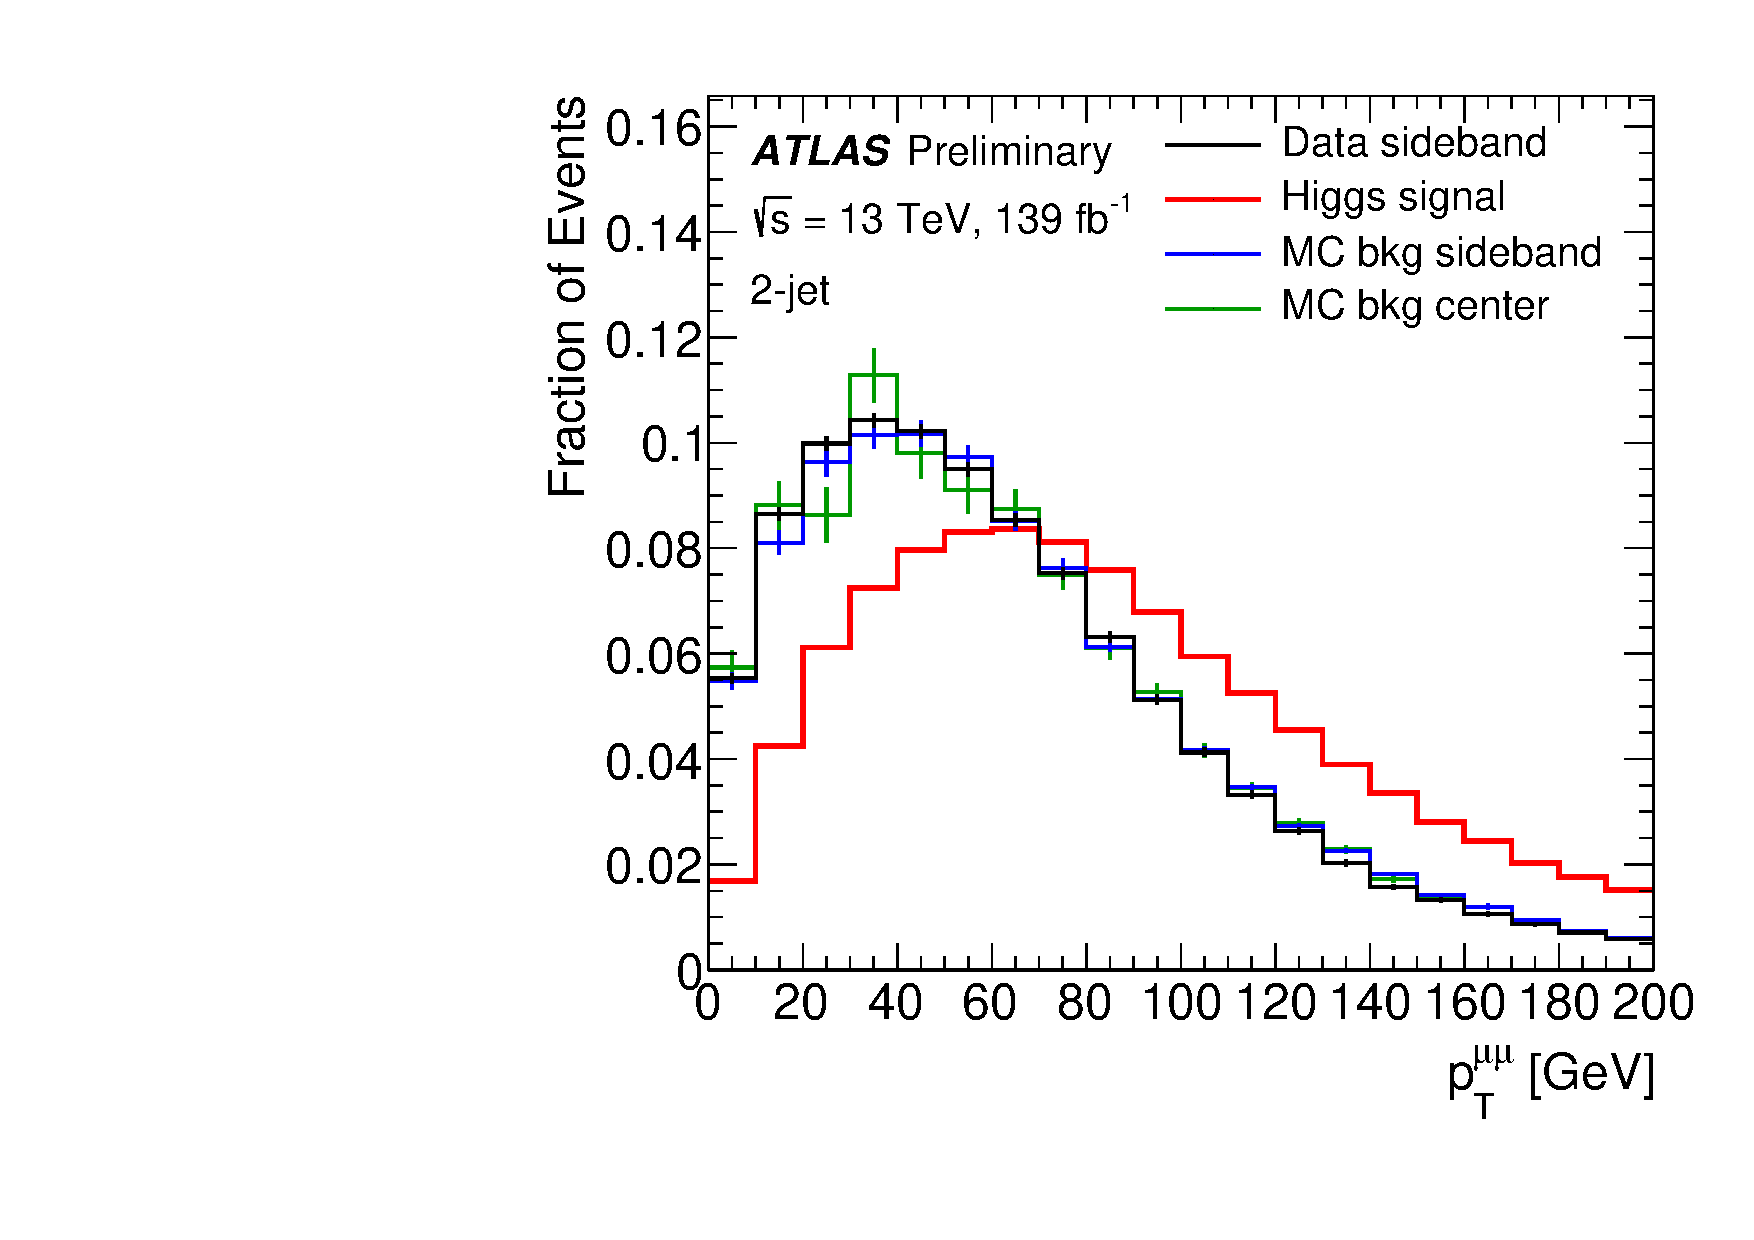
\includegraphics[width=0.3\textwidth]{figures/hmumu/vars/Z_PT_FSR}
  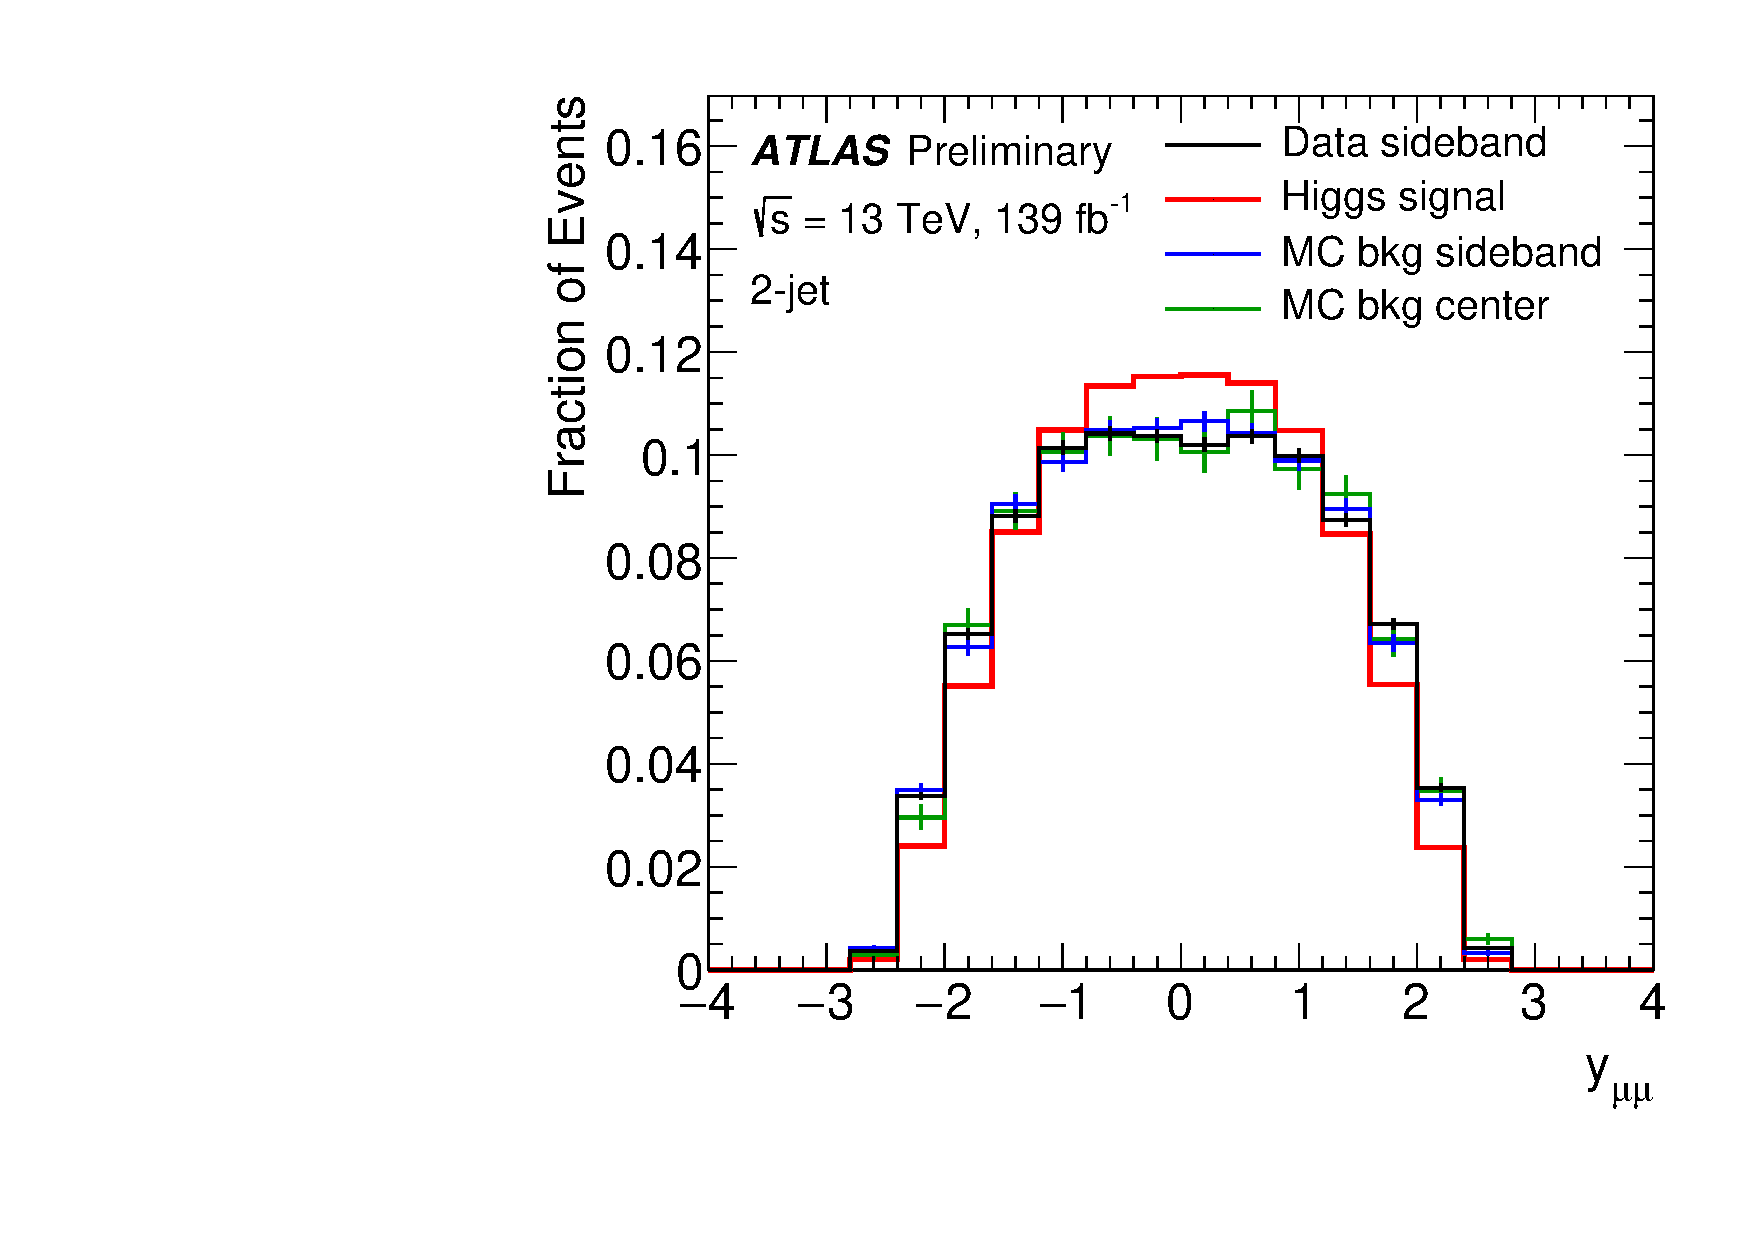
\includegraphics[width=0.3\textwidth]{figures/hmumu/vars/Z_Y_FSR}
  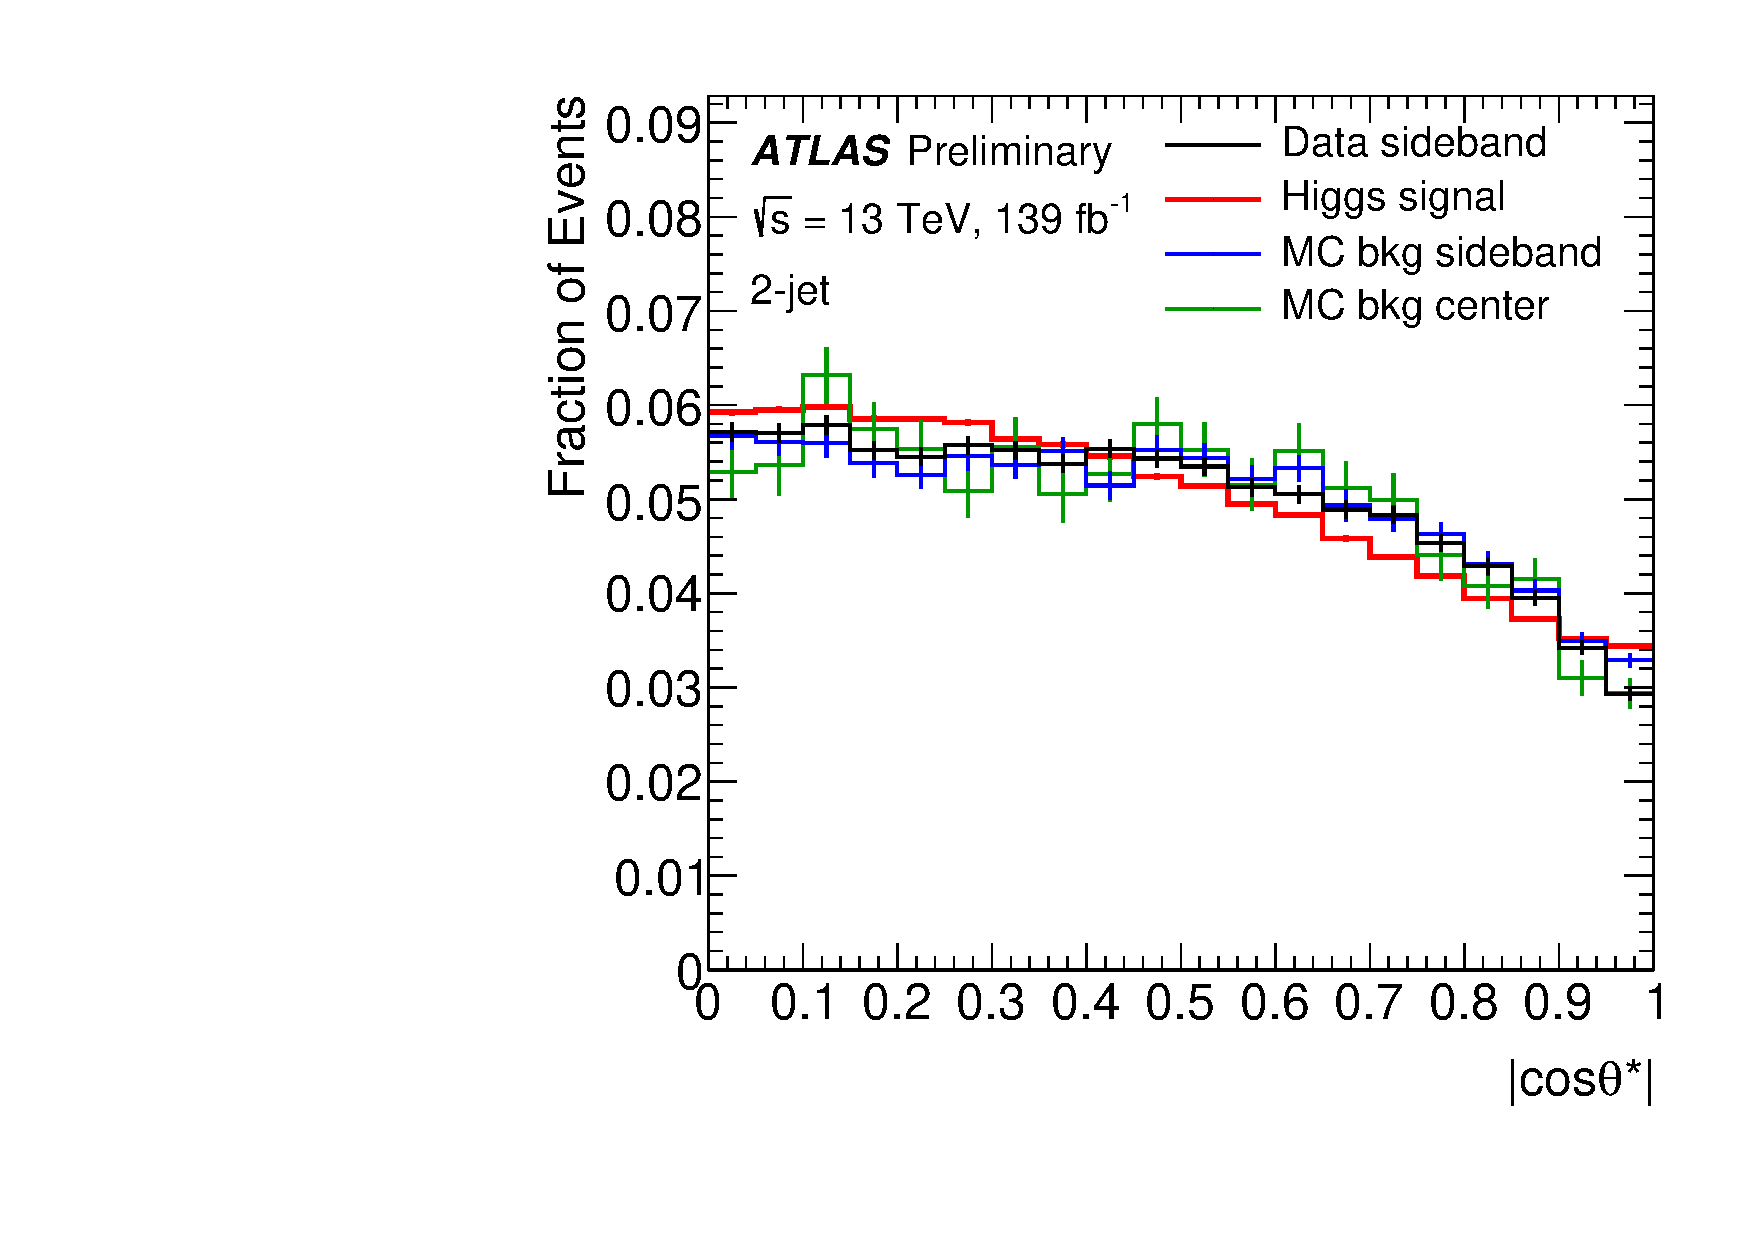
\includegraphics[width=0.3\textwidth]{figures/hmumu/vars/CosThetaStar} \\ 
  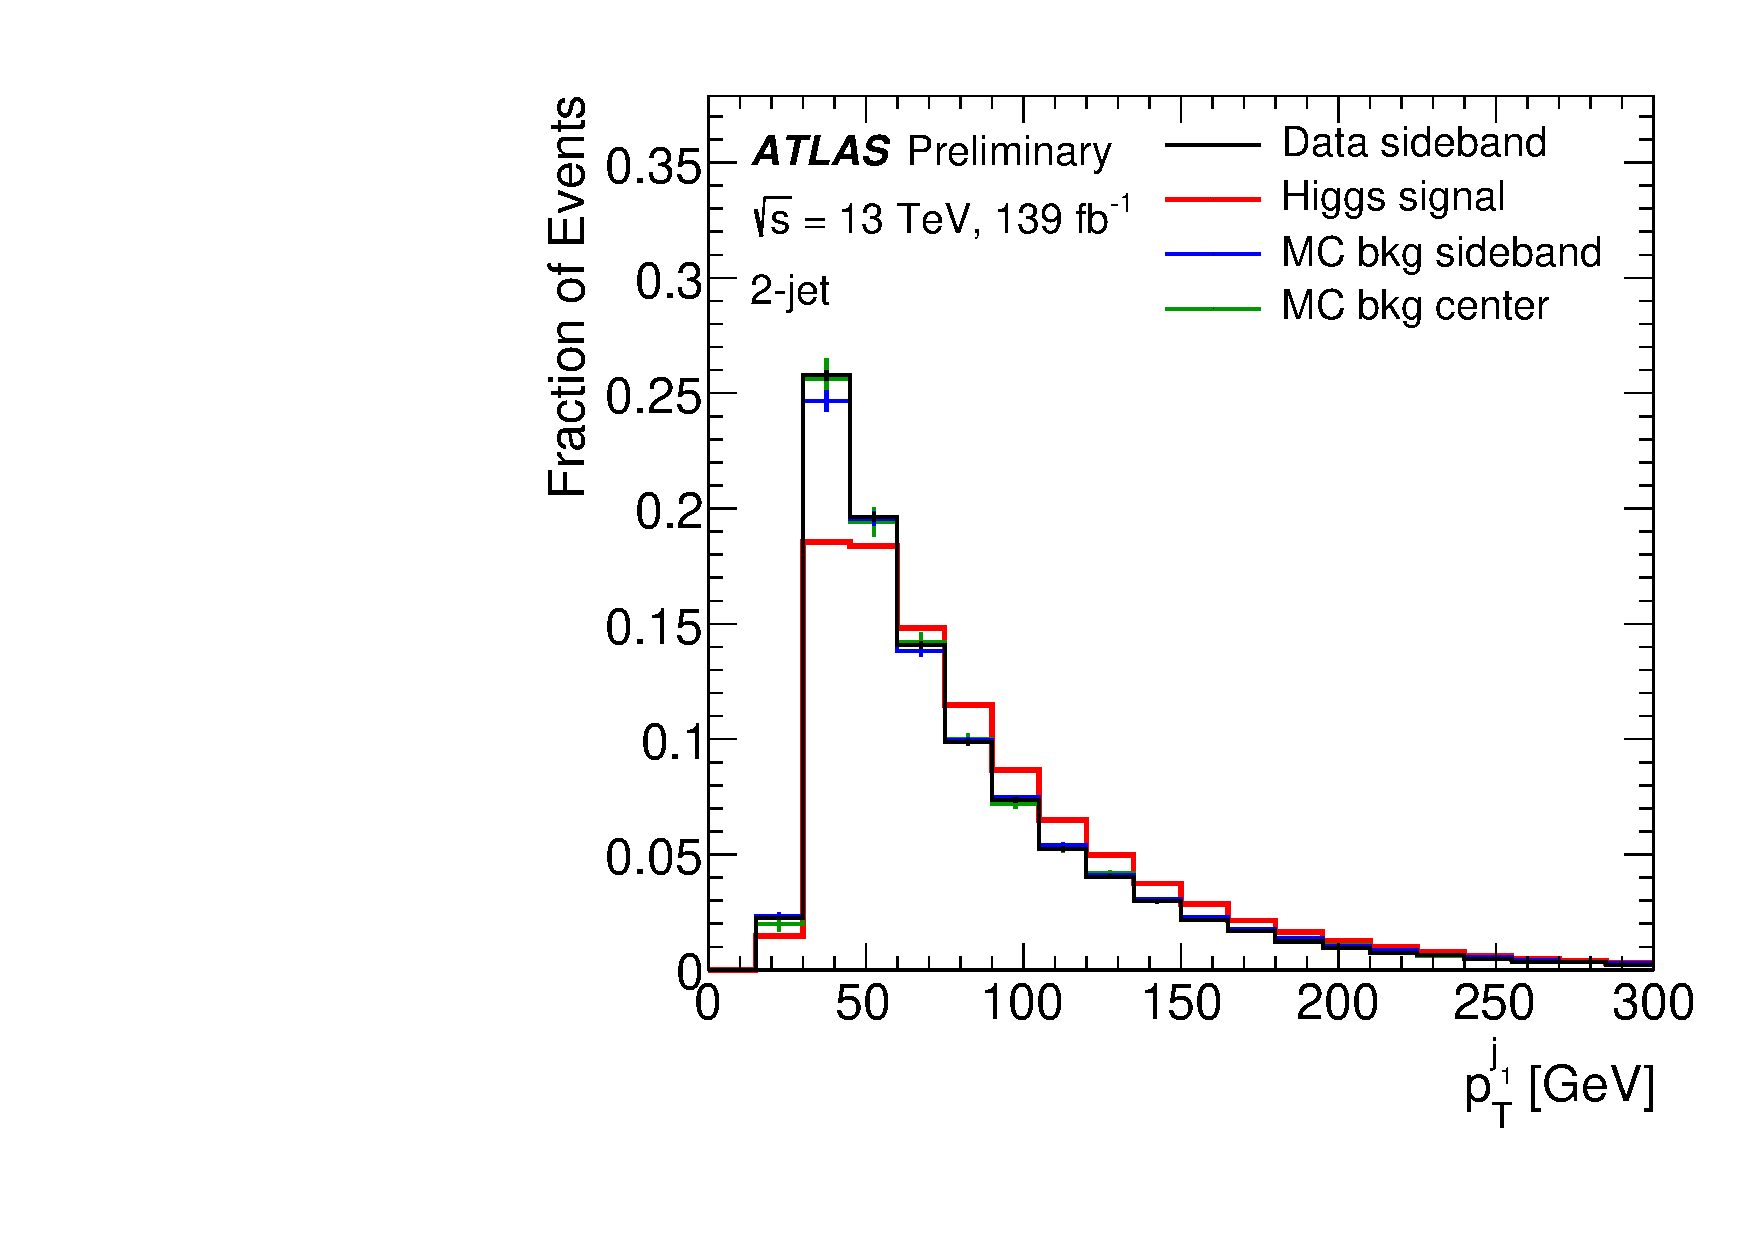
\includegraphics[width=0.3\textwidth]{figures/hmumu/vars/Jets_PT_Lead}
  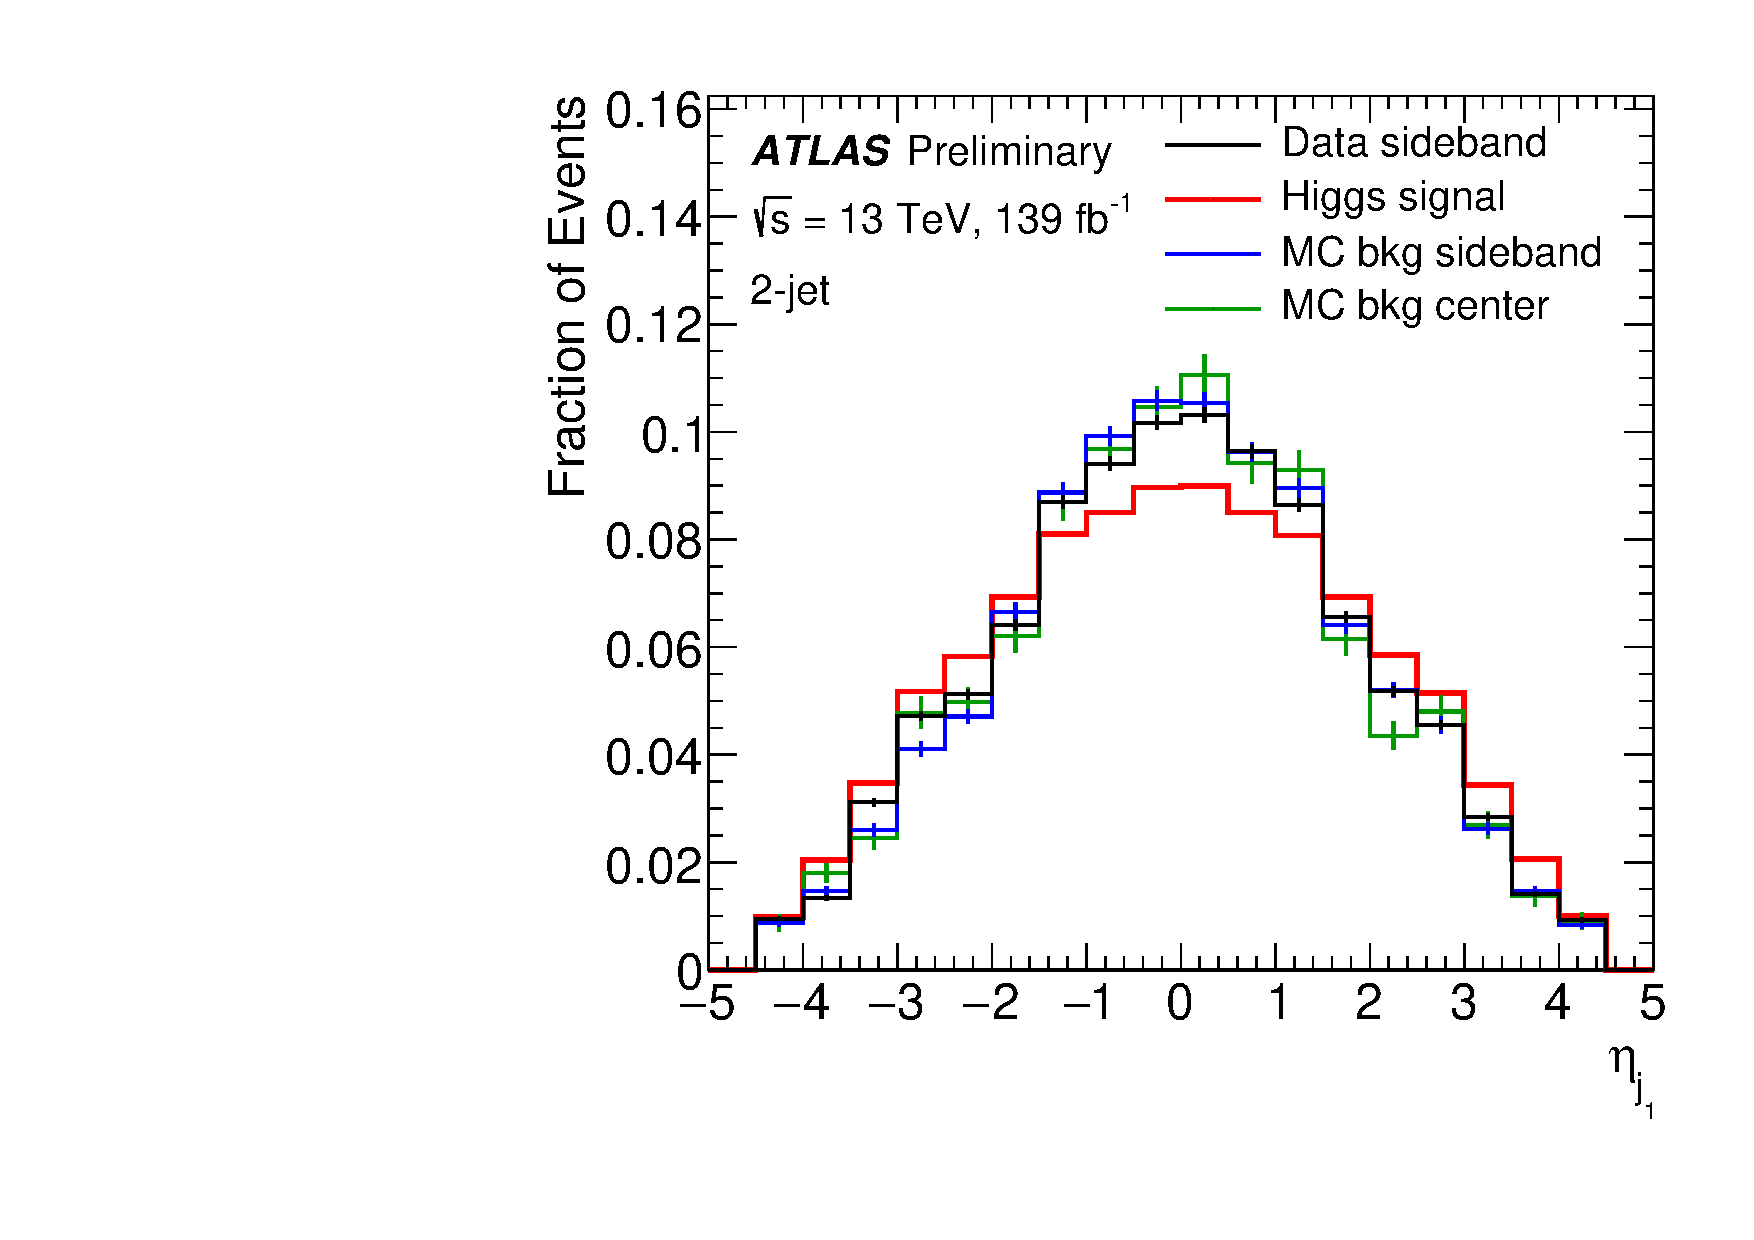
\includegraphics[width=0.3\textwidth]{figures/hmumu/vars/Jets_Eta_Lead}
  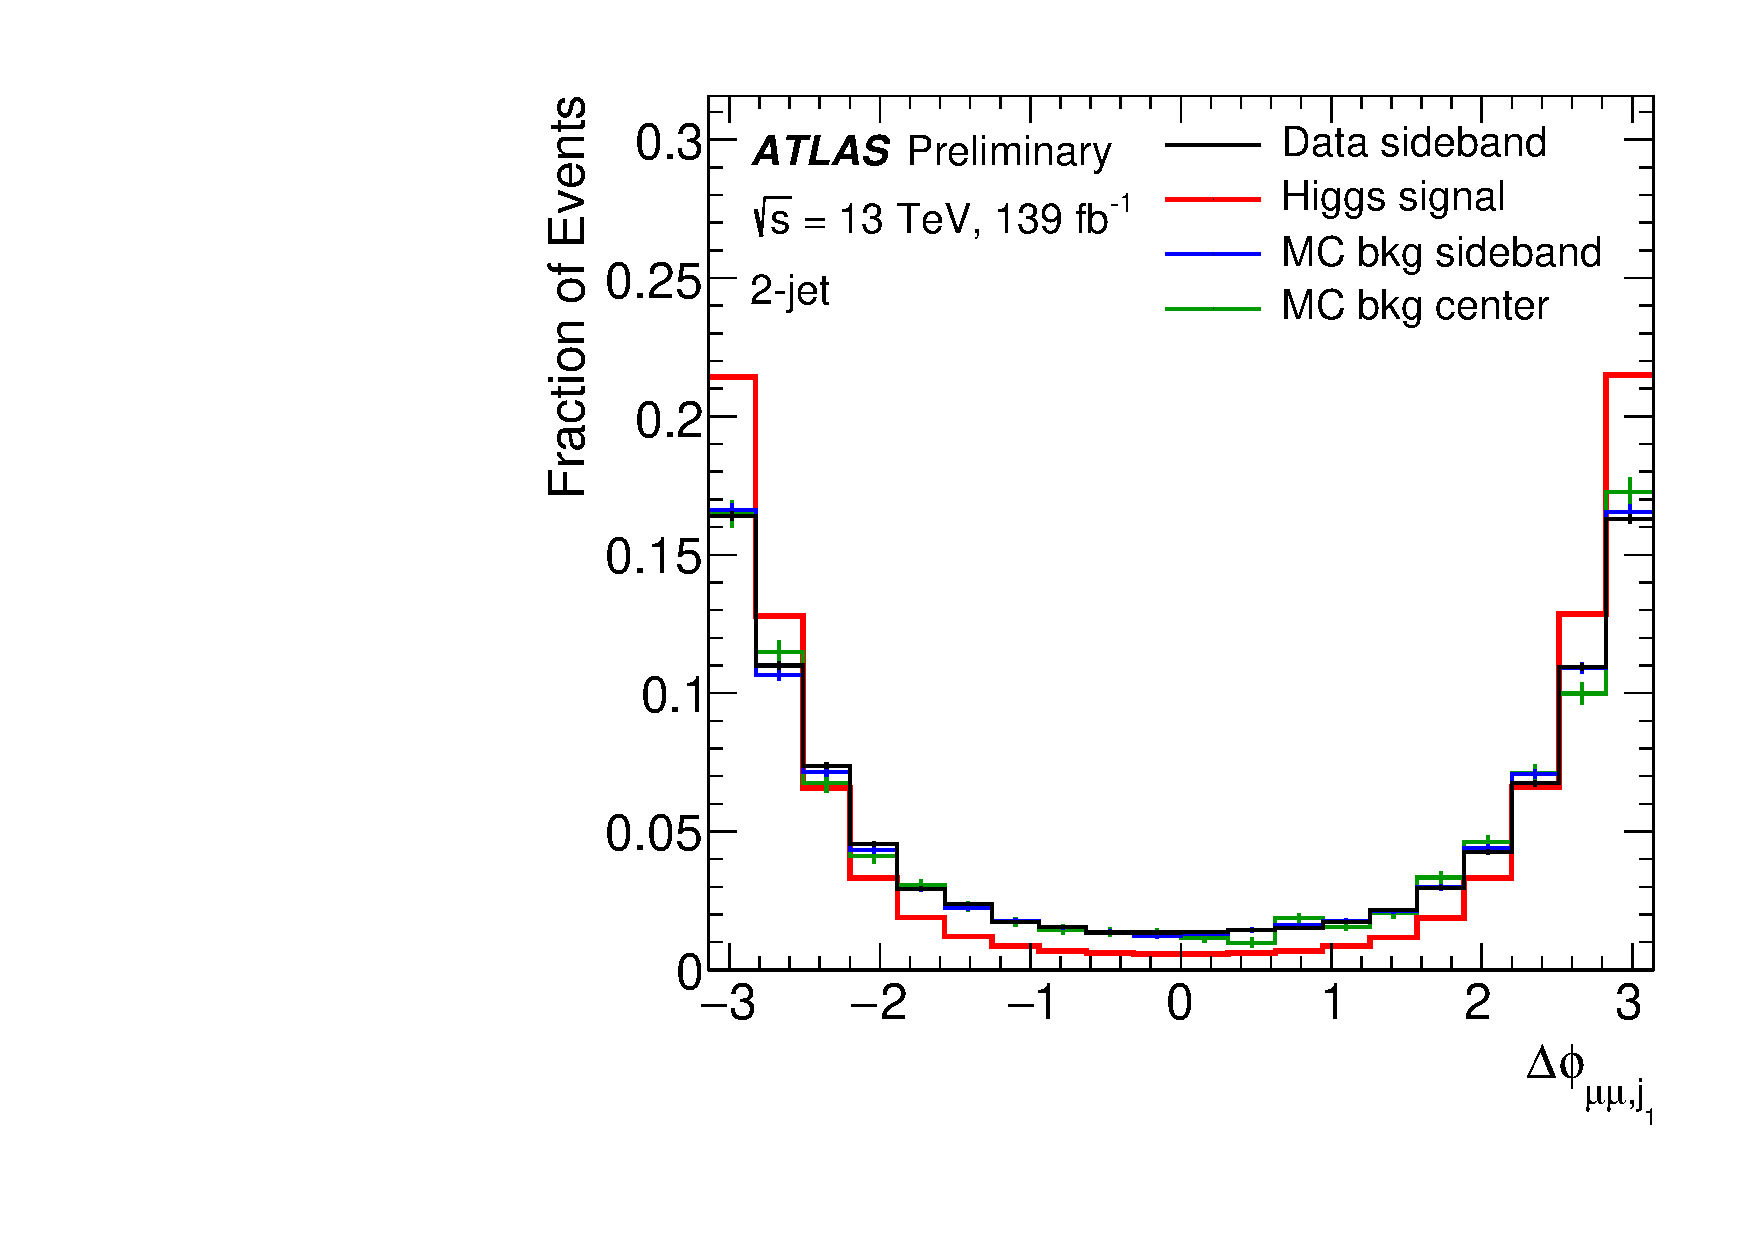
\includegraphics[width=0.3\textwidth]{figures/hmumu/vars/DeltaPhi_mumuj1} \\ 
  \caption[Classifier input variables]{
  Distributions of classifier
  input variables for events with two or more jets. Top row shows dimuon
  system variables, bottom row shows leading jet variables. $\hmumu$ signal events
  are shown in red, data from the sidebands are shown in black, and MC
  simulation of background events is shown blue (sideband region) and
  green (central region). MC simulation includes DY, diboson, and top events.
  Error bars are statistical. From Ref. \cite{ATLAS-CONF-2019-028}.
  }
  \label{fig:hmumu:variables01}
\end{figure}

\begin{figure}[h!]
  \centering
  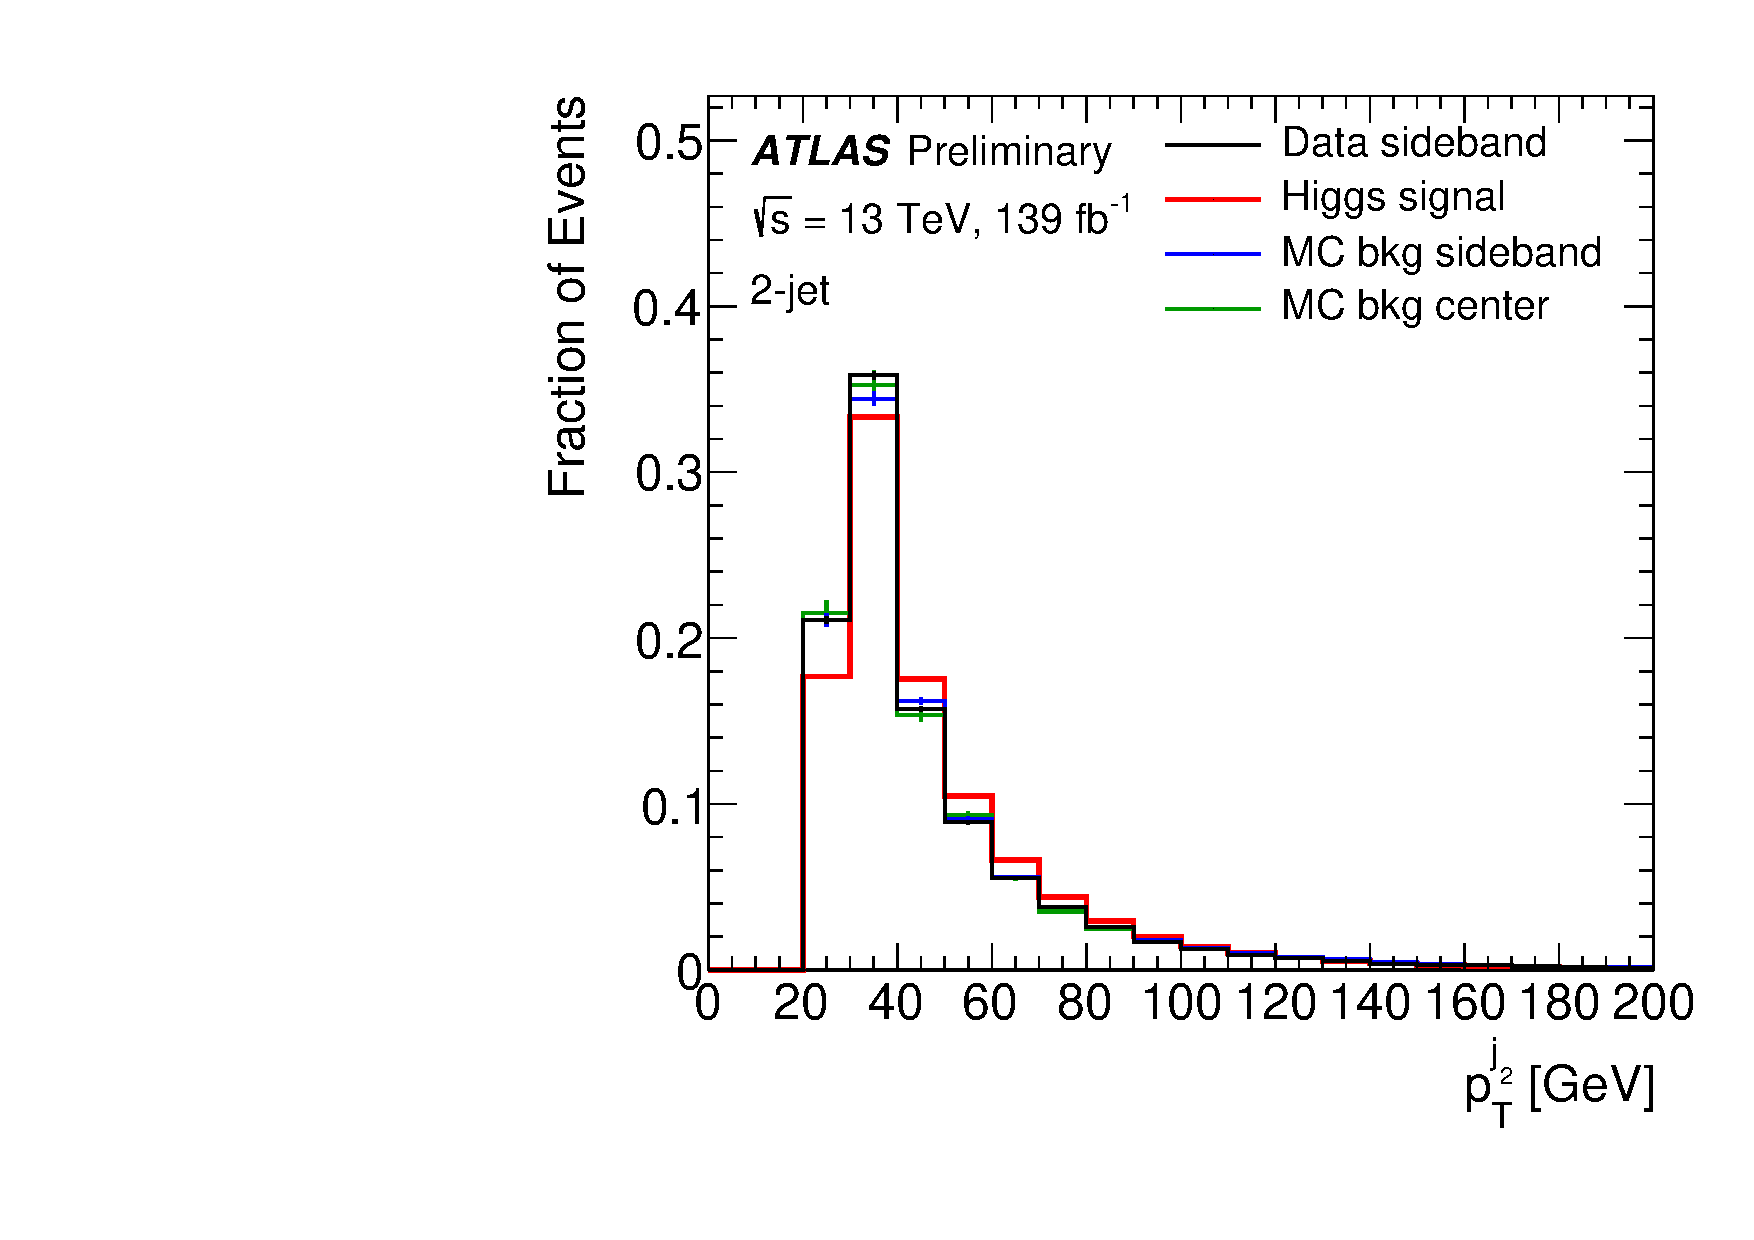
\includegraphics[width=0.3\textwidth]{figures/hmumu/vars/Jets_PT_Sub}
  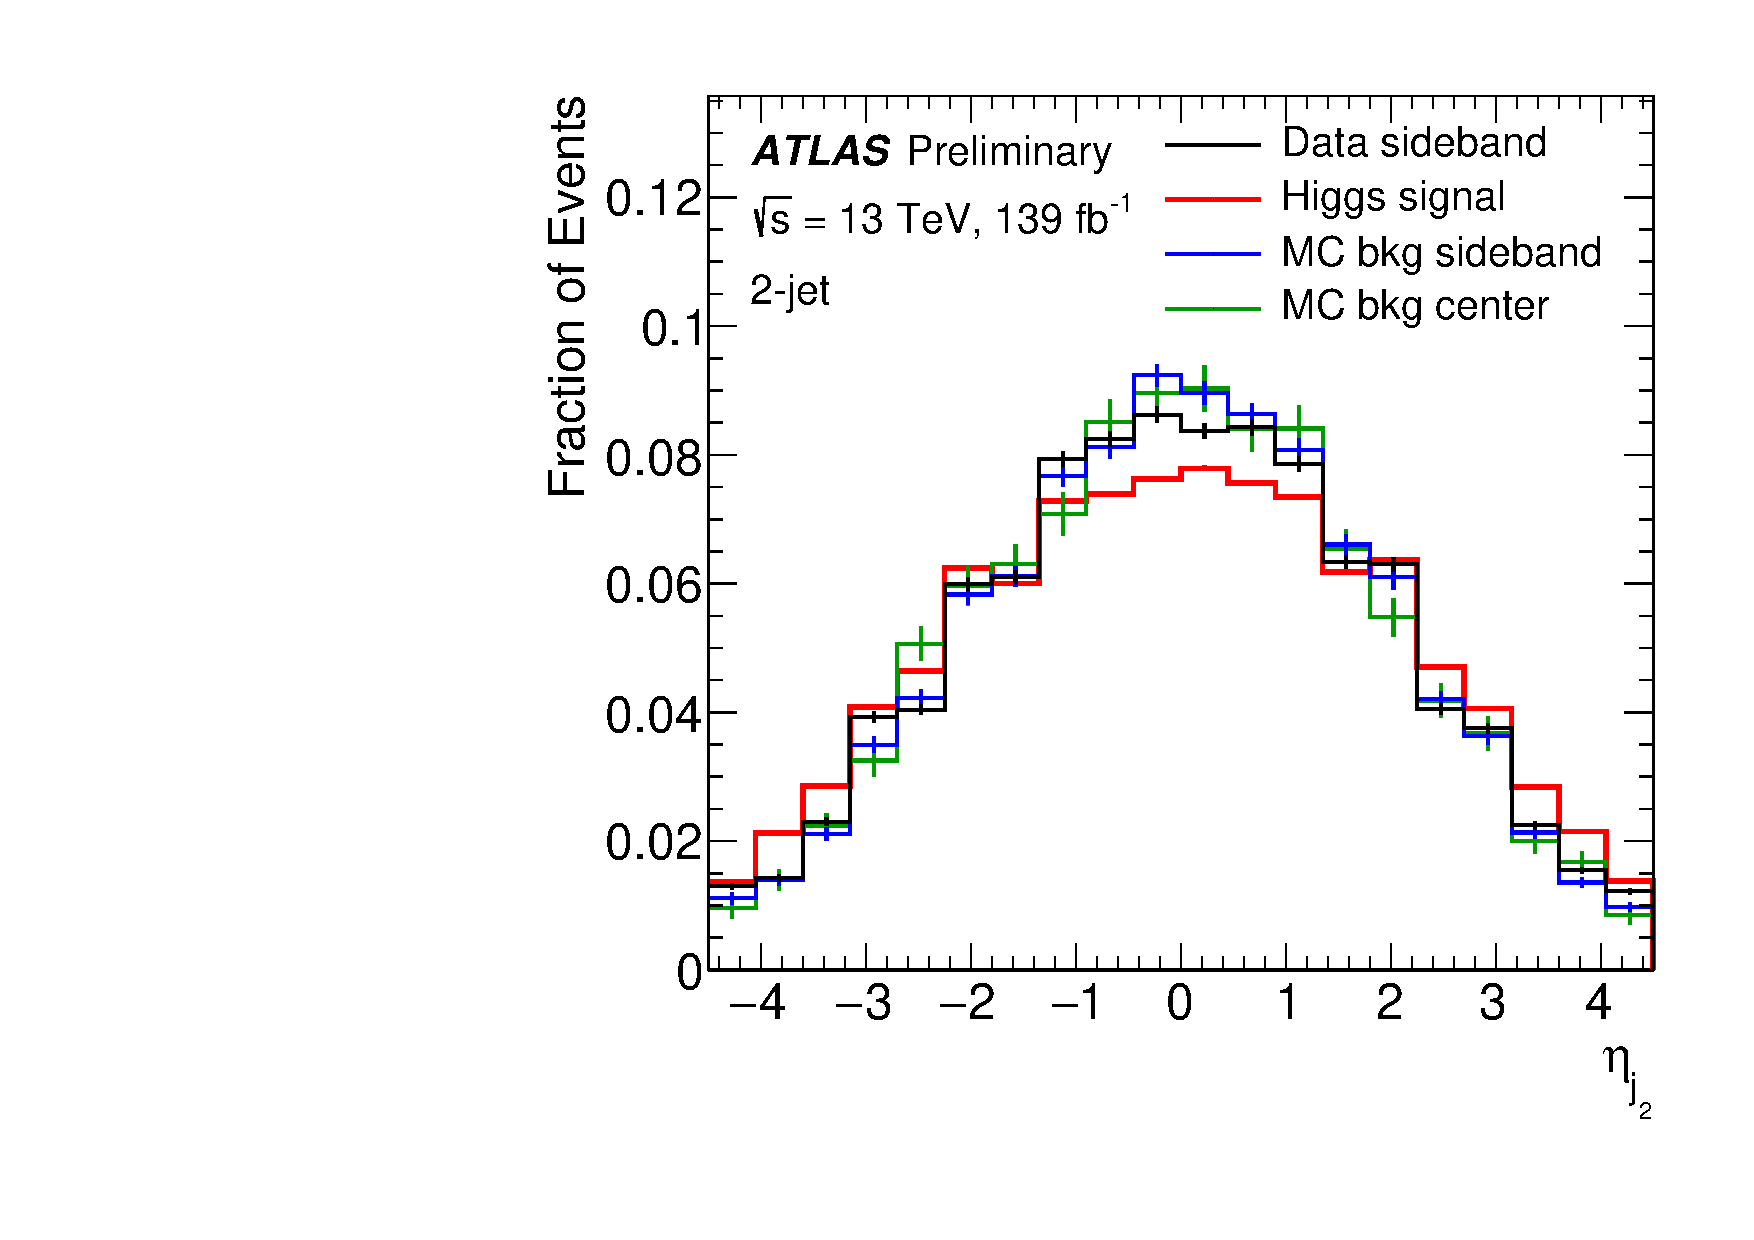
\includegraphics[width=0.3\textwidth]{figures/hmumu/vars/Jets_Eta_Sub}
  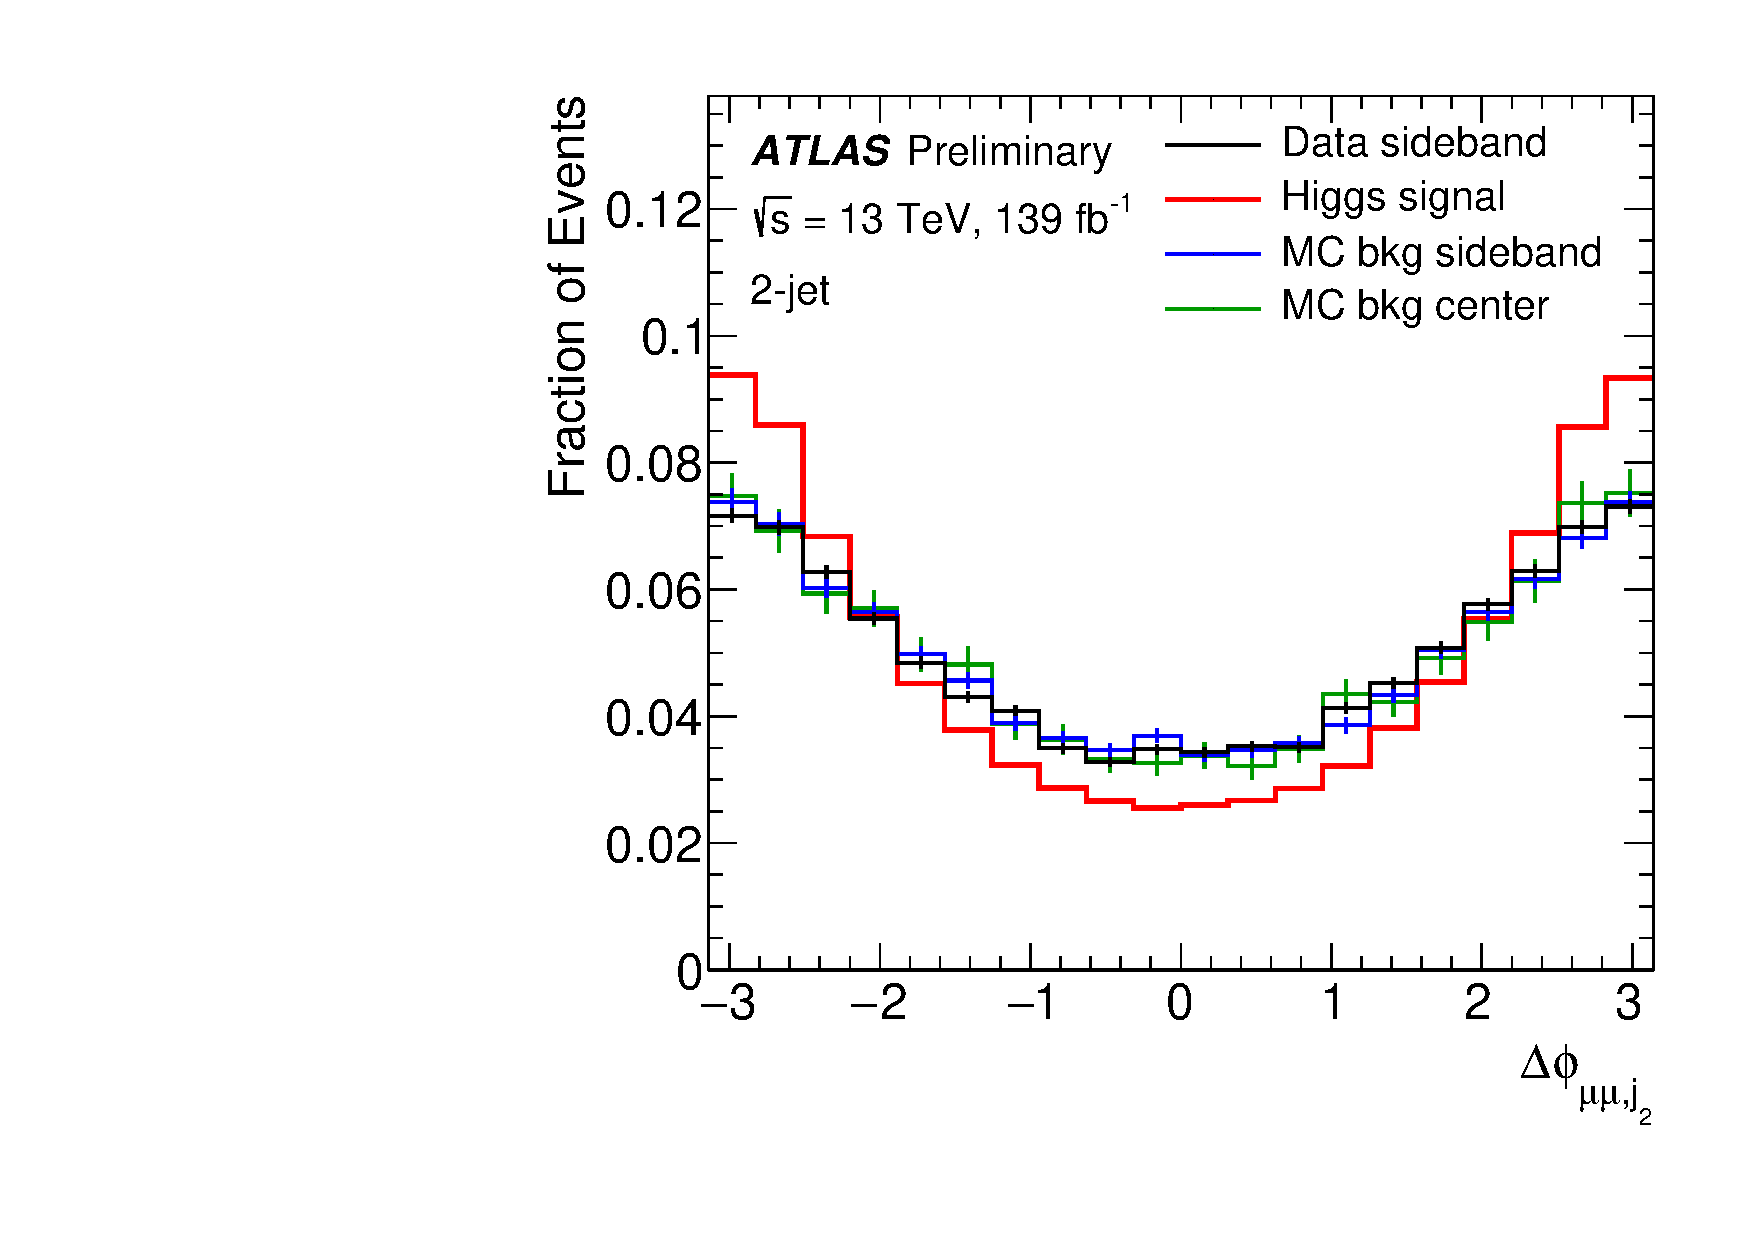
\includegraphics[width=0.3\textwidth]{figures/hmumu/vars/DeltaPhi_mumuj2} \\
  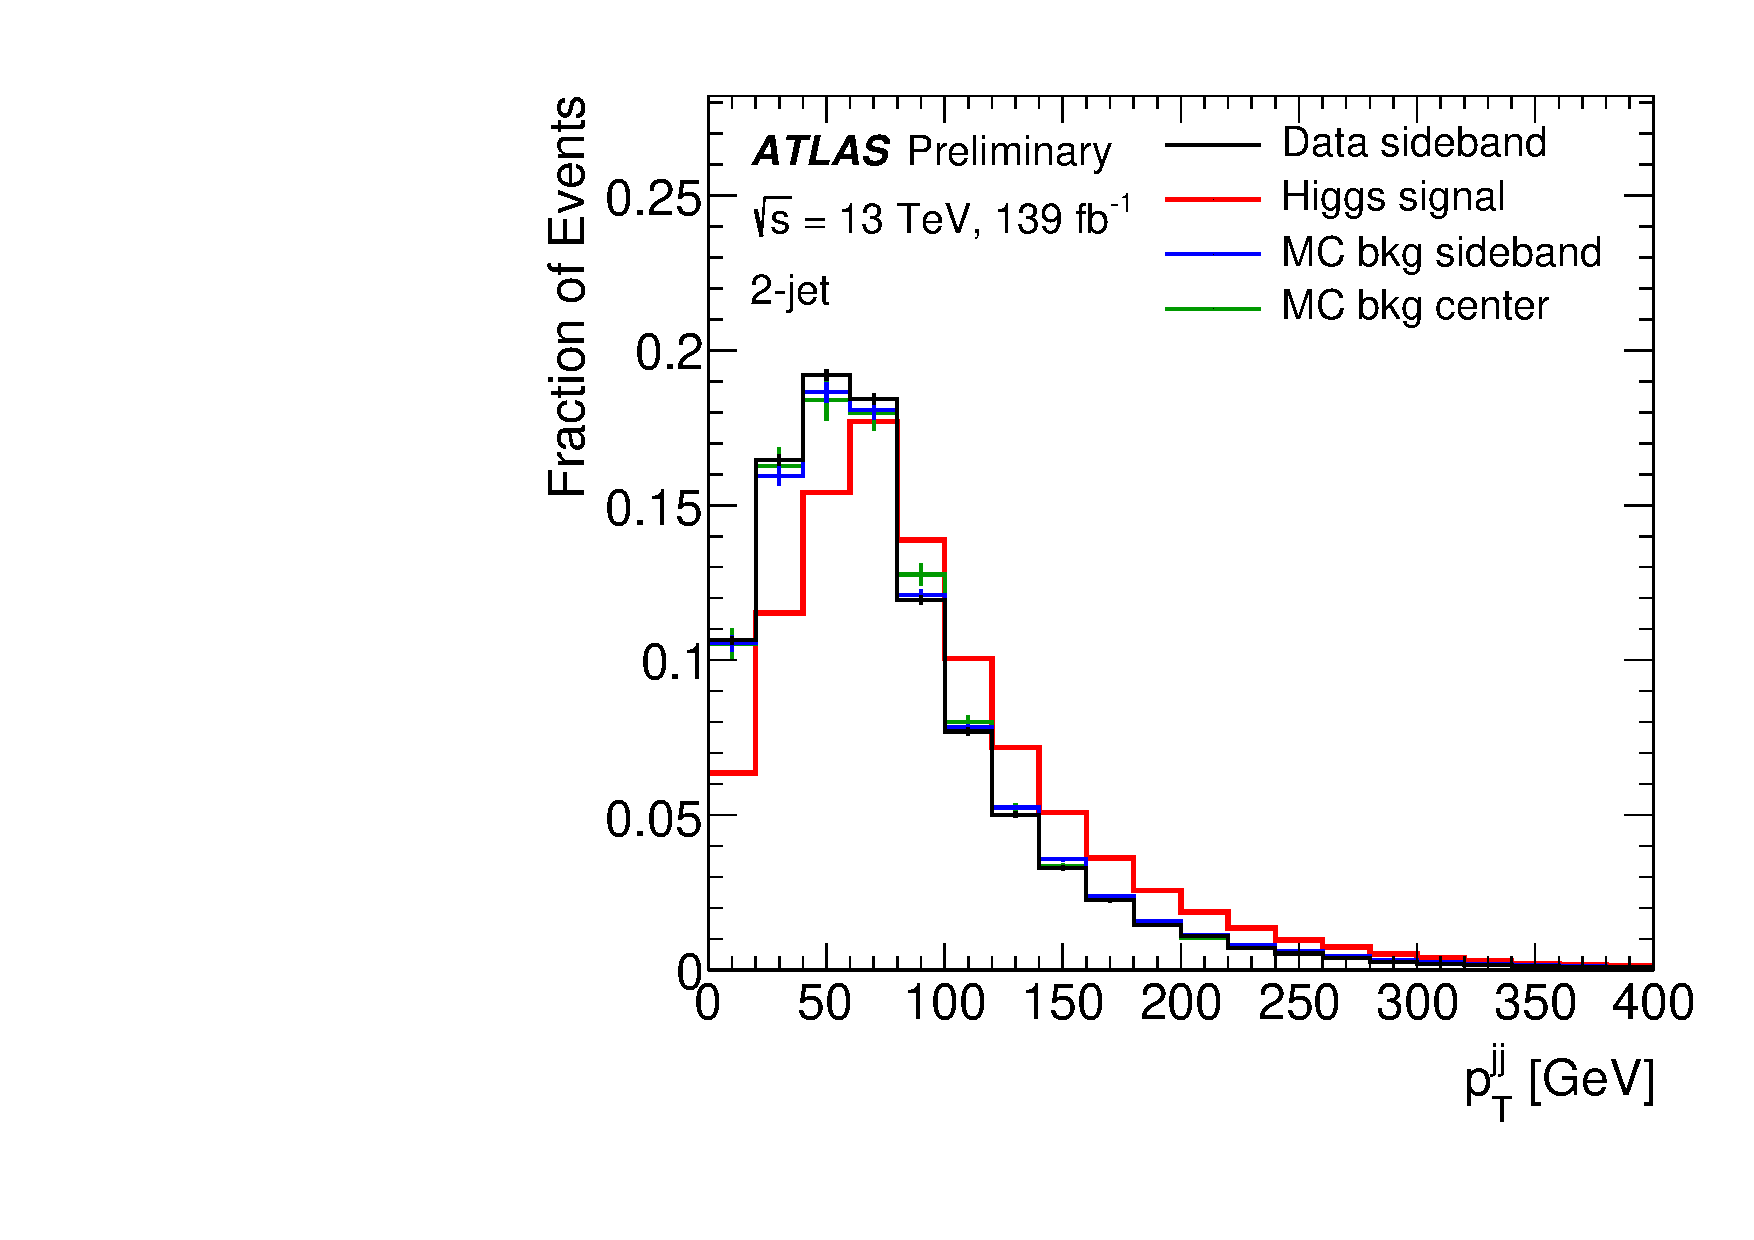
\includegraphics[width=0.3\textwidth]{figures/hmumu/vars/Jets_PT_jj}
  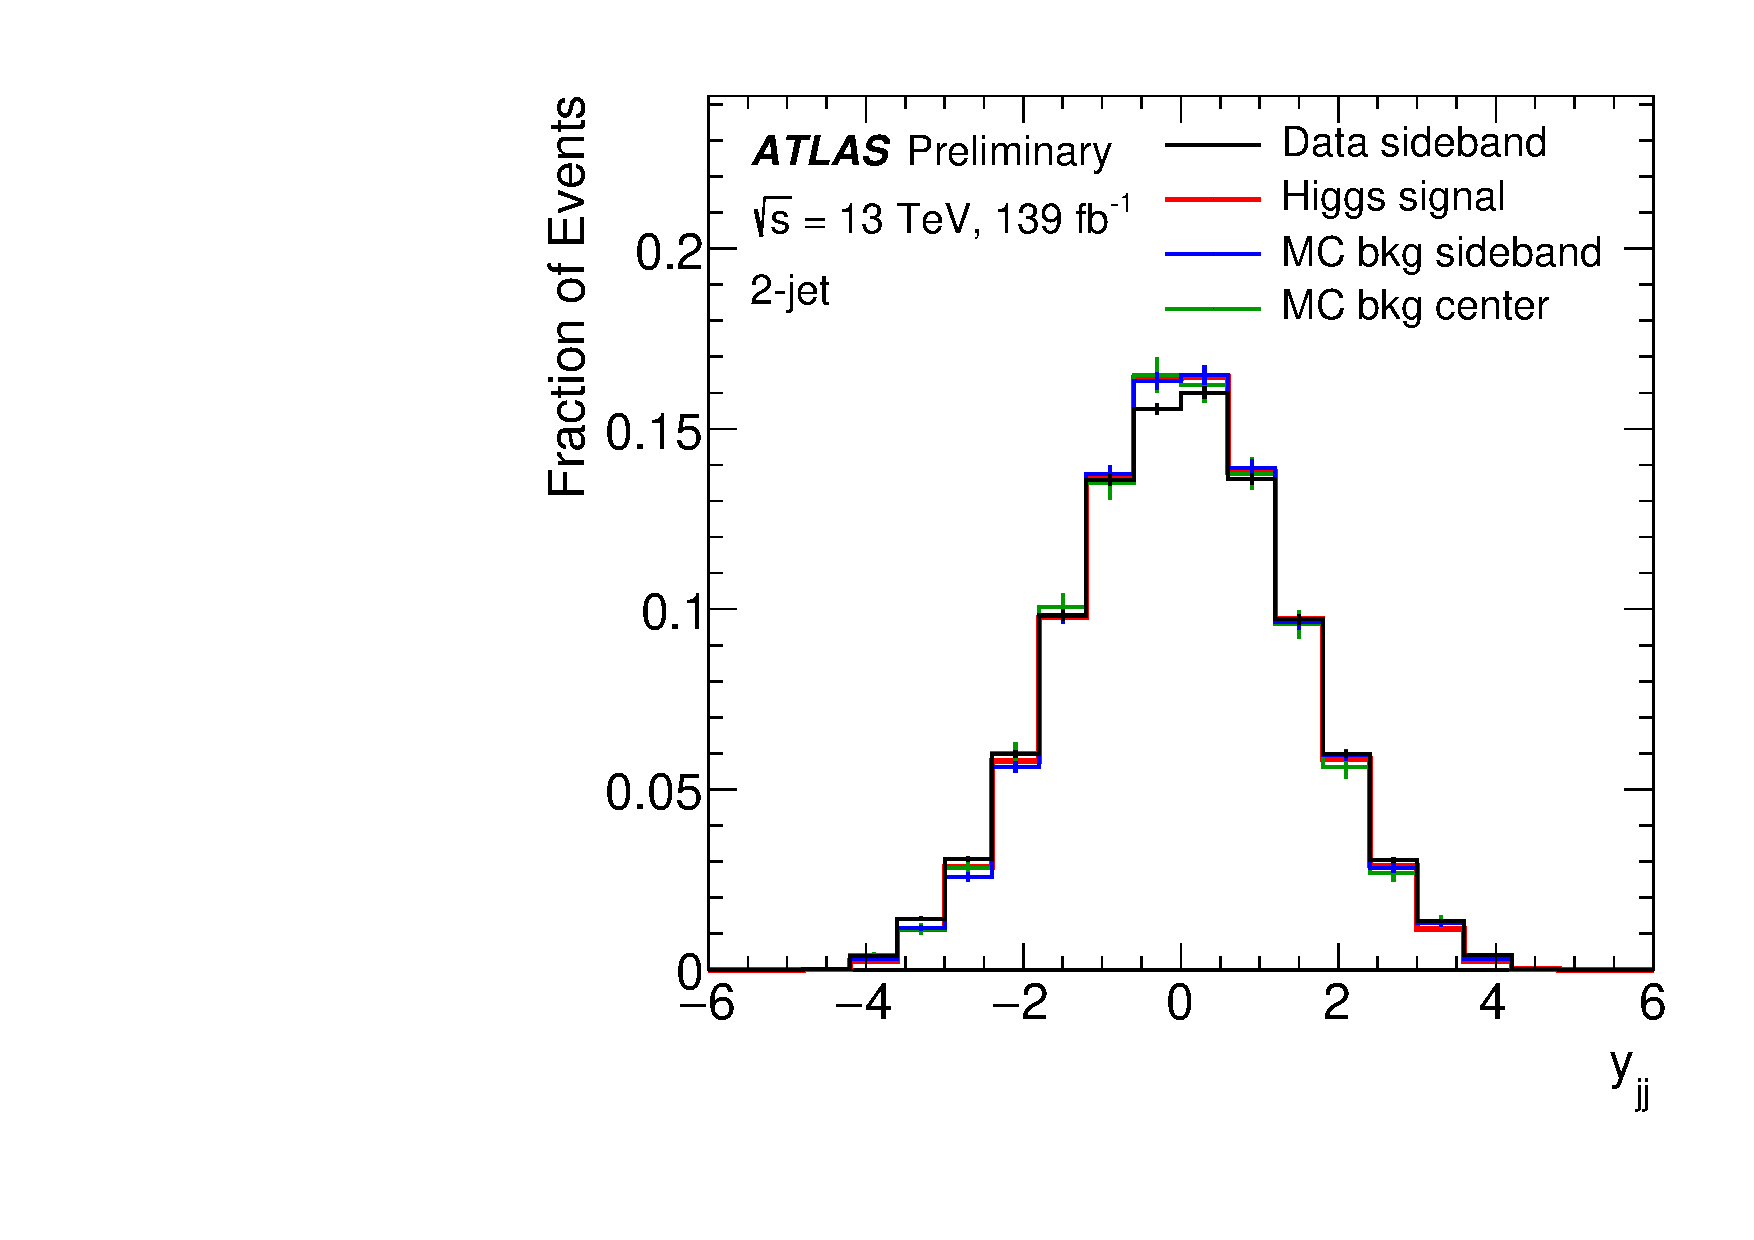
\includegraphics[width=0.3\textwidth]{figures/hmumu/vars/Jets_Y_jj}
  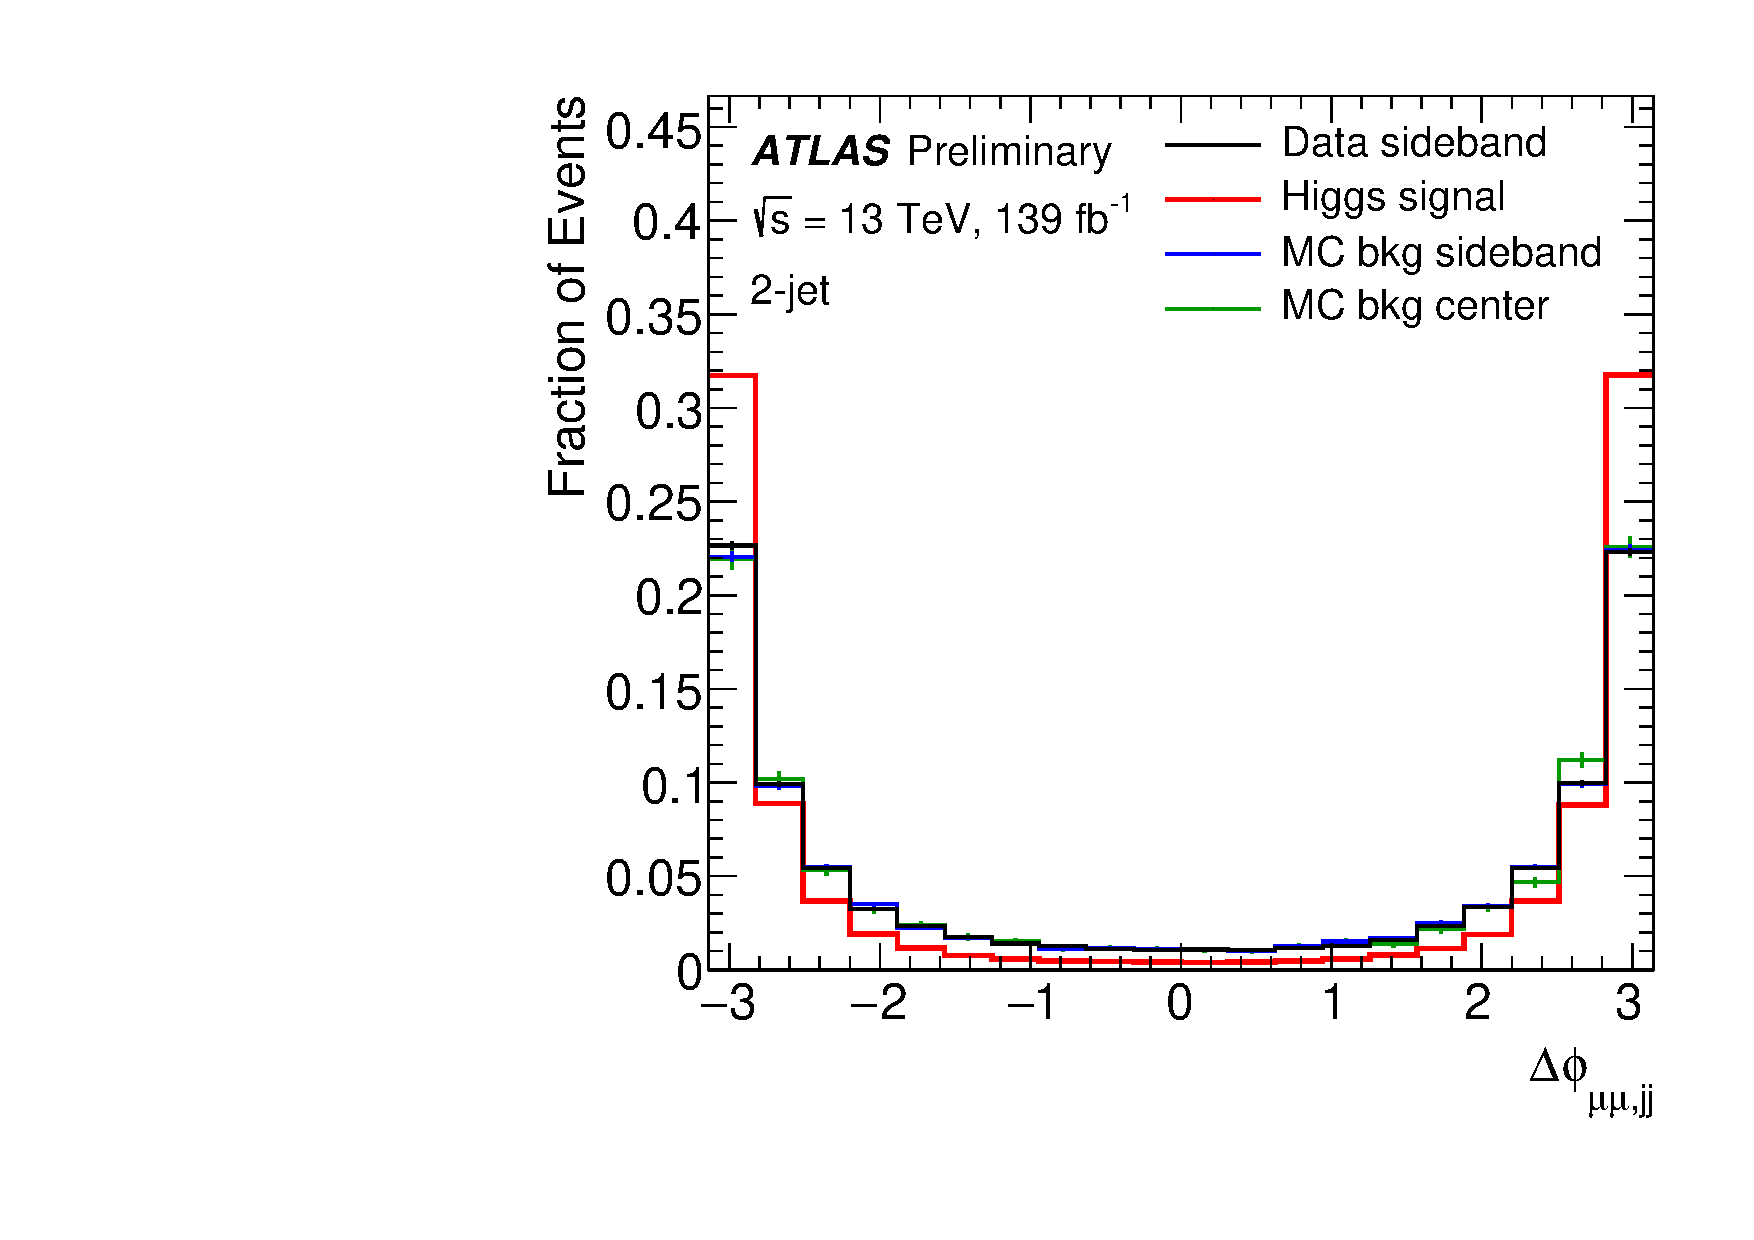
\includegraphics[width=0.3\textwidth]{figures/hmumu/vars/DeltaPhi_mumujj} \\
  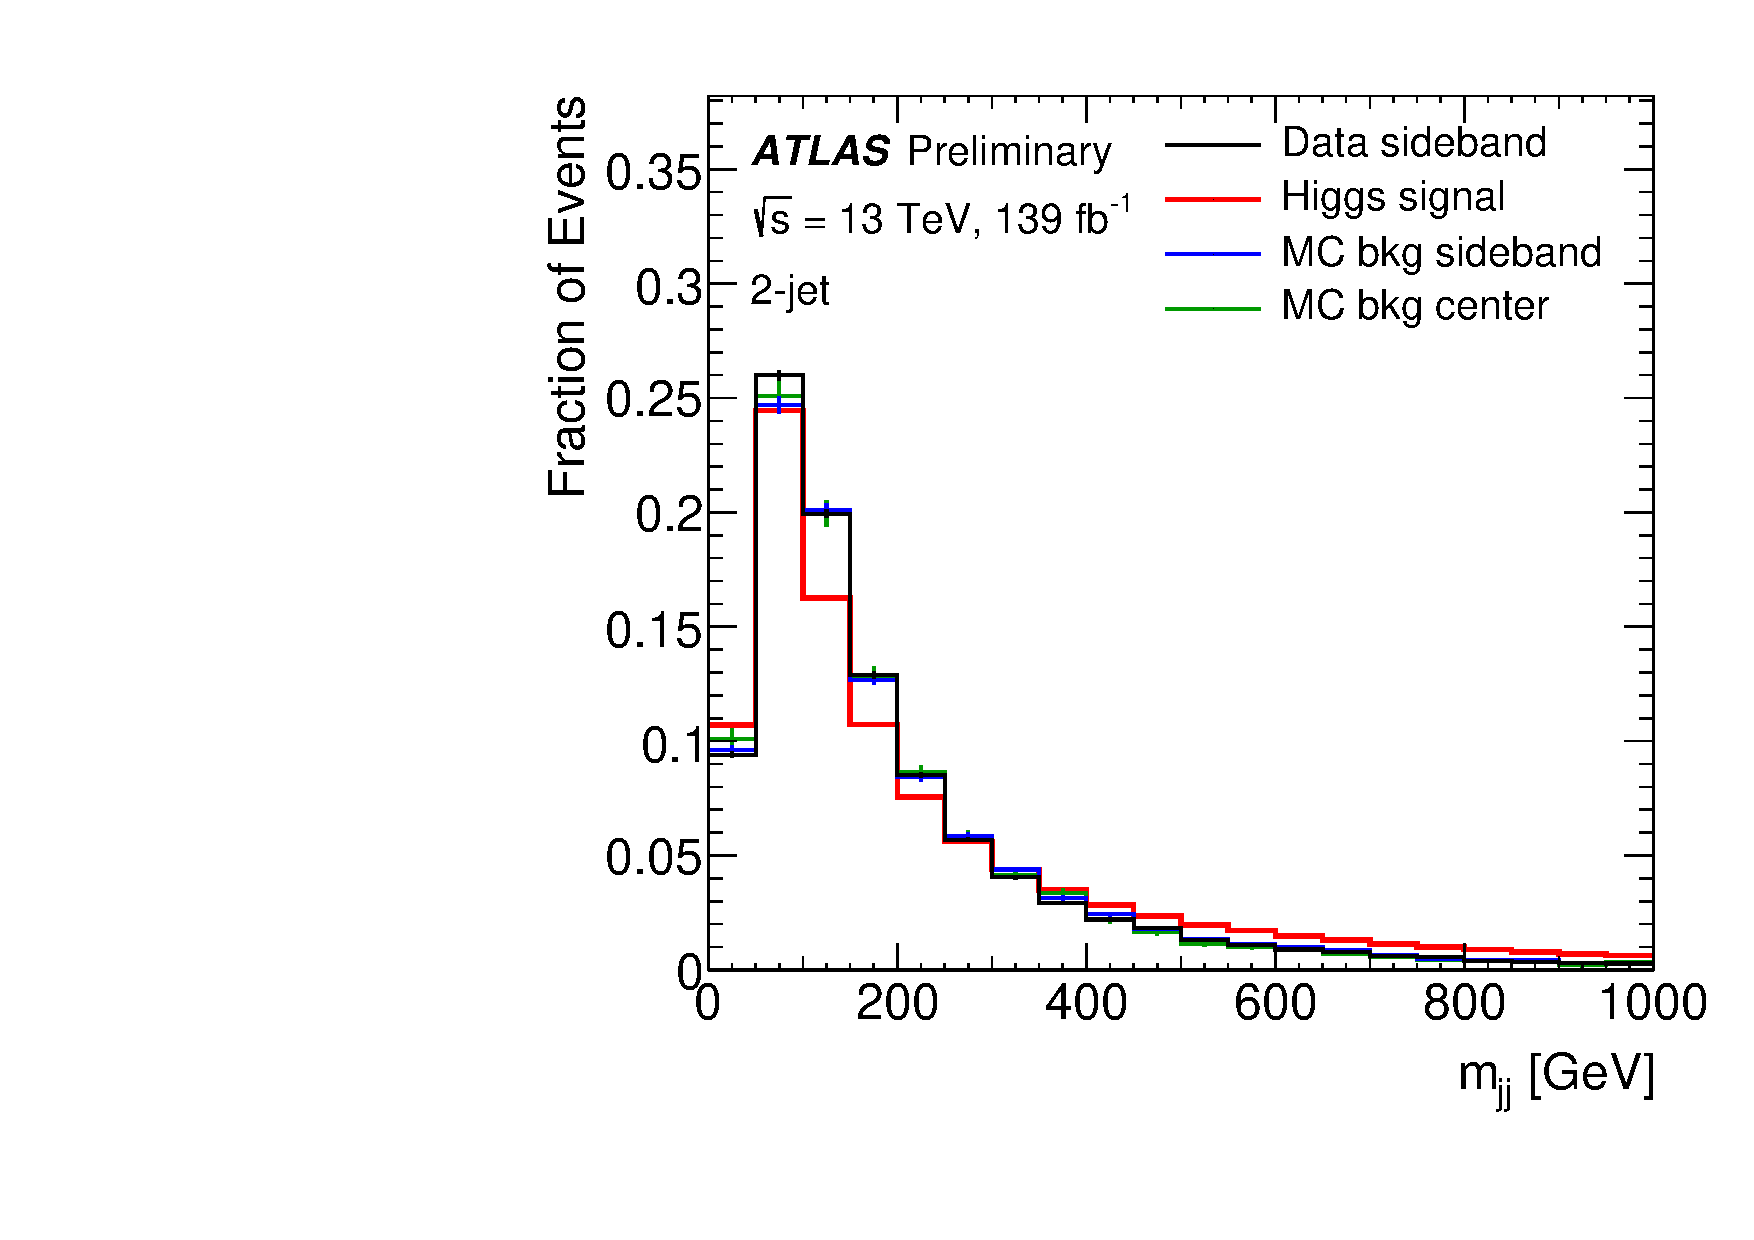
\includegraphics[width=0.3\textwidth]{figures/hmumu/vars/Jets_Minv_jj}
  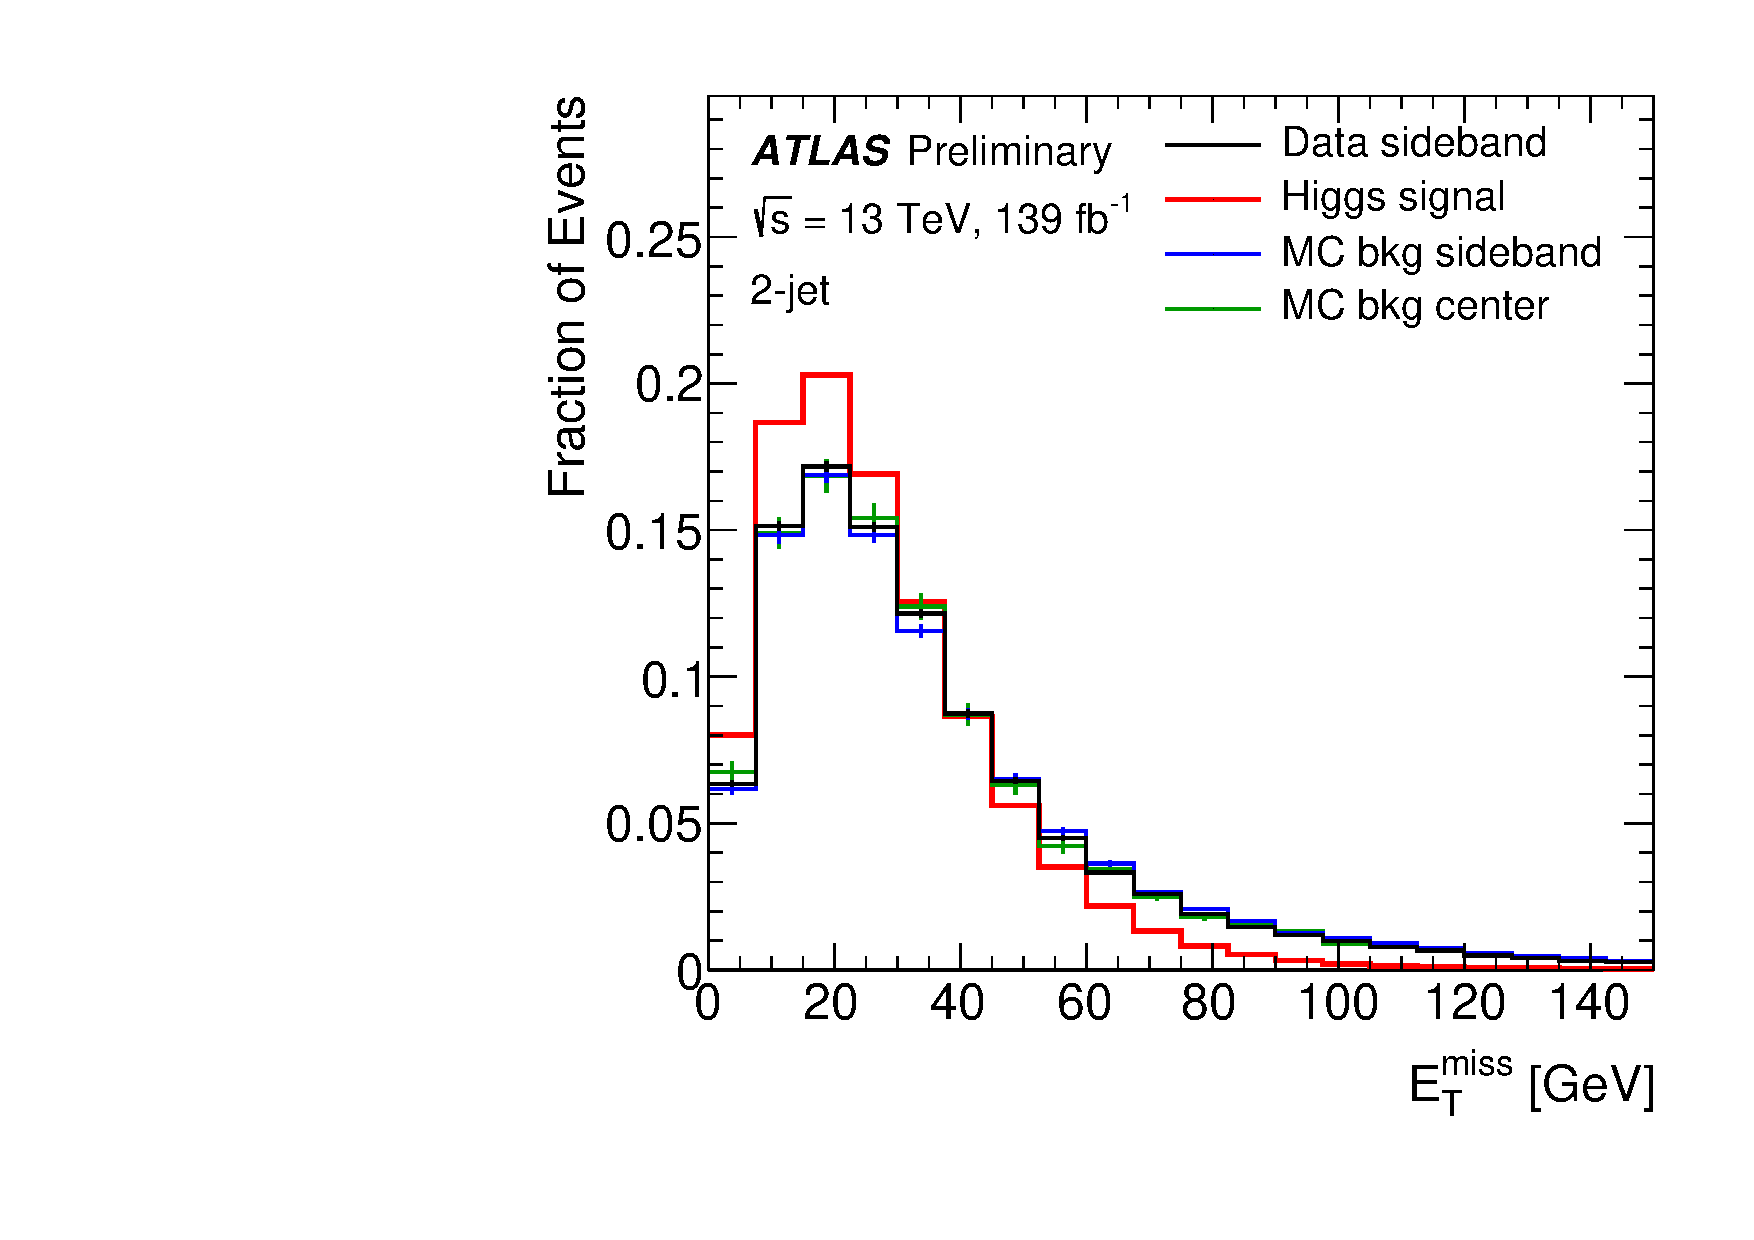
\includegraphics[width=0.3\textwidth]{figures/hmumu/vars/metFinalTrk}
  \caption[Classifier input variables]{
  Distributions of classifier
  input variables for events with two or more jets. Top row shows subleading
  jet variables, middle row dijet system variables, bottom row shows the
  dijet invariant mass and $\met$. $\hmumu$ signal events
  are shown in red, data from the sidebands are shown in black, and MC
  simulation of background events is shown blue (sideband region) and
  green (central region). MC simulation includes DY, diboson, and top events.
  Error bars are statistical. From Ref. \cite{ATLAS-CONF-2019-028}.
  }
  \label{fig:hmumu:variables2}
\end{figure}

In each jet multiplicity channel a four-fold approach is used to
prevent bias from overfitting to the training and validation sets.
In each fold, events are split in a training set (50\% of events),
a validation set (25\% of events), and a test set (25\% of events).
Training set is used in the training of the models. The validation
set is used for early stopping of the training and to assess the
performance of models using the area under the ROC
\cite{journals/prl/Fawcett06} curve. This is used to guide the
Bayesian optimisation \cite{gp} to tune the hyperparameters of the
model in each fold. Finally, the model is evaluated on the test set,
which is used for the categorisation of events.

It should be noted that in the four-fold approach the model parameters
are selected separately in each fold. This results in four models,
each being applied to the test set not seen in training, early stopping,
or hyperparameter tuning, ensuring that there is no bias from overfitting
to either training or validation datasets.

In order to ensure that the score distributions are the same in each
fold, the scores are transformed to a uniform distribution in unweighted
combined signal events in all fold separately using the QuantileTransformer
algorithm from the \texttt{scikit-learn} \cite{scikit-learn} software package.

The transformed scores are named $O_\text{VBF}$ for the VBF classifier,
and $O_\ggf^(0-2)$ for the Higgs classifiers, where the superscript
stands for the jet multiplicity. The category boundaries are defined
as the cuts on these values, and are summarised in Table \ref{tab:hmumu:categories}.
\begin{table}[h]
\centering
\caption{Summary of the score boundaries defining the analysis categories.}
\label{tab:hmumu:categories}
\begin{tabular}{c c c c}
\toprule
\midrule
%       &    0-jet                       &      1-jet                     & 2-jet ($O_\text{VBF} < 0.60$) & VBF \\
%High   & $O^0_{\ggf} \geq 0.75$         & $O^1_{\ggf} \geq 0.78$         & $O^2_{\ggf} \geq 0.48$          & $O_\text{VBF} \geq 0.89$ \\
%Medium & $0.35 \leq O^0_{\ggf} < 0.75$  & $0.38 \leq O^1_{\ggf} < 0.78$  & $0.22 \leq O^2_{\ggf} < 0.48$   & $0.77 \leq O_\text{VBF} < 0.89$ \\
%Low    & $O^0_{\ggf} < 0.35$            & $O^1_{\ggf} < 0.38$            & $O^2_{\ggf} < 0.22$             & $O_\text{VBF} < 0.77$ \\
                              & Low                   &  Medium                           &    High                  \\ 
\midrule
0-jet                         & $O^0_{\ggf} < 0.35$   &  $0.35 \leq O^0_{\ggf} < 0.75$    & $O^0_{\ggf} \geq 0.75$   \\
1-jet                         & $O^1_{\ggf} < 0.38$   &  $0.38 \leq O^1_{\ggf} < 0.78$    & $O^1_{\ggf} \geq 0.78$   \\
2-jet ($O_\text{VBF} < 0.60$) & $O^2_{\ggf} < 0.22$   &  $0.22 \leq O^2_{\ggf} < 0.48$    & $O^2_{\ggf} \geq 0.48$   \\
VBF                           & $O_\text{VBF} < 0.77$ &  $0.77 \leq O_\text{VBF} < 0.89$  & $O_\text{VBF} \geq 0.89$ \\
\midrule
\bottomrule
\end{tabular}
\end{table}

The values of category boundaries are determined by a simultaneous
optimisation of all boundaries in a given jet channel using an exhaustive
search over the cut value grid with 0.01 spacing. The metric used in the
optimisation is the number counting significance, defined as
\begin{equation}
Z = \sqrt{\sum_{c=1}^{12} 2 \left[ (s_c + b_c) \log \left( \frac{s_c+b_c}{b_c}\right) - s_c \right]},
\end{equation}
where the sum runs over categories $c$, and $s_c$ and $b_c$ are the
number of signal and background events in the central region in category
$c$. Since the optimisation is performed blinded, the value of $b_c$ is
computed from the number of data events in the sideband region, multiplied
by a transfer factor obtained from the inclusive MC distribution.

The summary of analysis categories is shown in Figure \ref{fig:hmumu:cat-summary},
highlighting the composition of signal and background events, as well
as the signal purity (S/B) and sensitivity proxy (S/$\sqrt{\text{B}}$),
and the total number of background events (B) in the central region for
all the analysis categories, where S is the expected number of signal events
in the central region. The signal purity decreases from High to
Low categories, while the number of background events decreases. The
significance proxy is approximately constant, which is a result of the 
optimisation rather than a requirement.
\begin{figure}[h!]
  \centering
  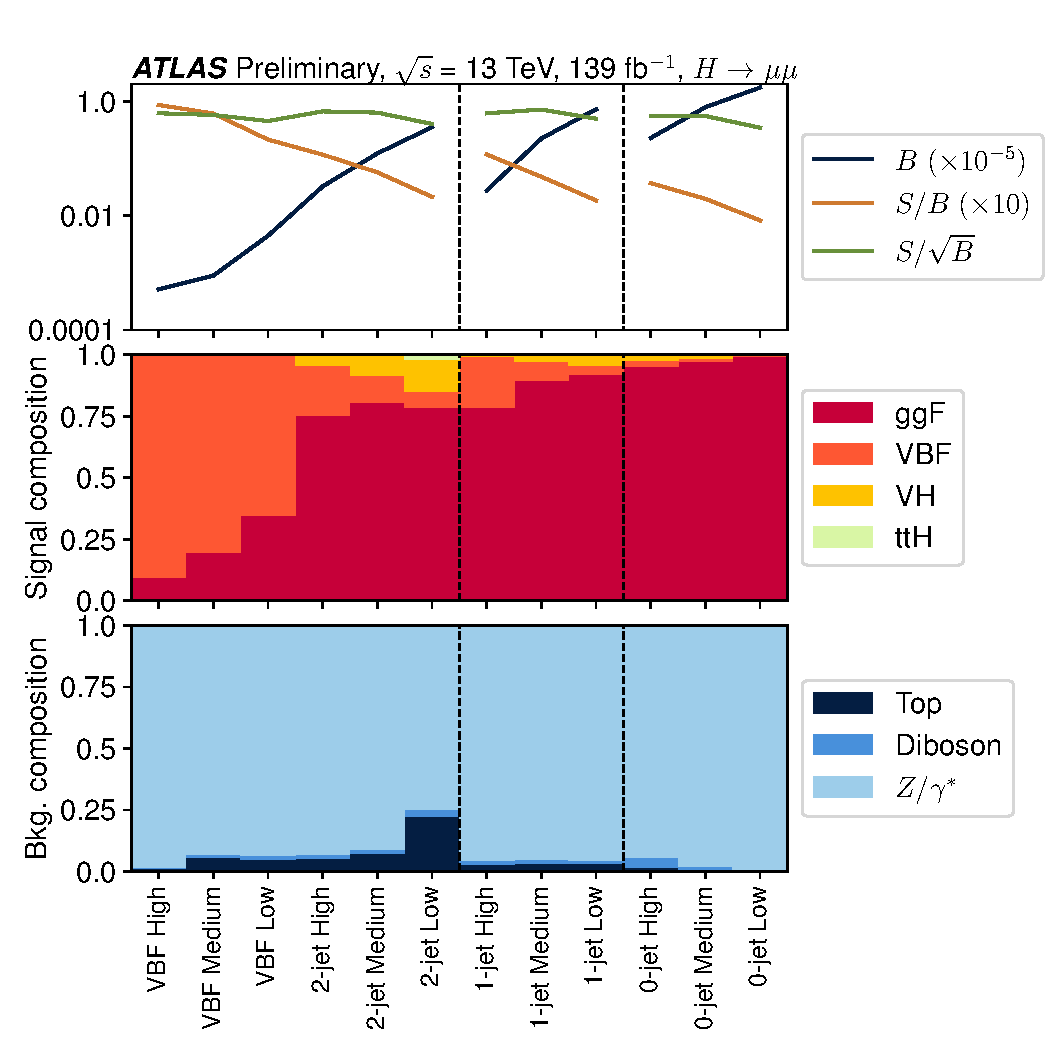
\includegraphics[width=1.0\textwidth]{figures/hmumu/cat-summary}
  \caption[Summary of $\hmumu$ analysis categories]{Summary of $\hmumu$
  analysis categories. Top panel shows the total number of background events
  in the central region, multiplied by $10^{-5}$ for visibility in blue,
  while the signal purity, multiplied by 10, is shown in orange and the
  significance proxy in green. The middle panel shows the signal
  composition of the categories, dominated by VBF events, shown in orange,
  in the VBF targetting categories, and by $\ggf$ events, shown in red,
  in all the others. VH events are shown in yellow, and $\tth$ events
  in lime. The background composition in shown in the bottom 
  panel and is dominated by DY events, shown in light blue. Diboson events
  are shown in blue, and top events in dark blue. From Ref. \cite{ATLAS-CONF-2019-028}.
  }
  \label{fig:hmumu:cat-summary}
\end{figure}

As explored in VADER4$\mu$ project, the momentum resolution of muons
is a function of their kinematics. Furthermore, the categorisation of
events in the analysis is based on a BDT classifier, which exploits
the kinematic differences between the signal and background events.
As a result, the analysis categories can have quite different
invariant mass resolutions. While this is expected, it is critical
that the modelling of dimuon mass resolution in MC simulation matches
the resolution in data in each analysis category, otherwise the
sensitivity would be over or under estimated. The validation of
the momentum calibrations, described in Section \ref{sec:muons:calibration},
is performed on the $Z$ mass peak. The validation for 0-jet High,
1-jet High, 2-jet High, and VBF High categories are shown in
Figure \ref{fig:hmumu:reso}. Bottom panels show that resolution
modelling is well within systematic uncertainties, similar results are
seen on other categories.
\begin{figure}[h!]
  \centering
  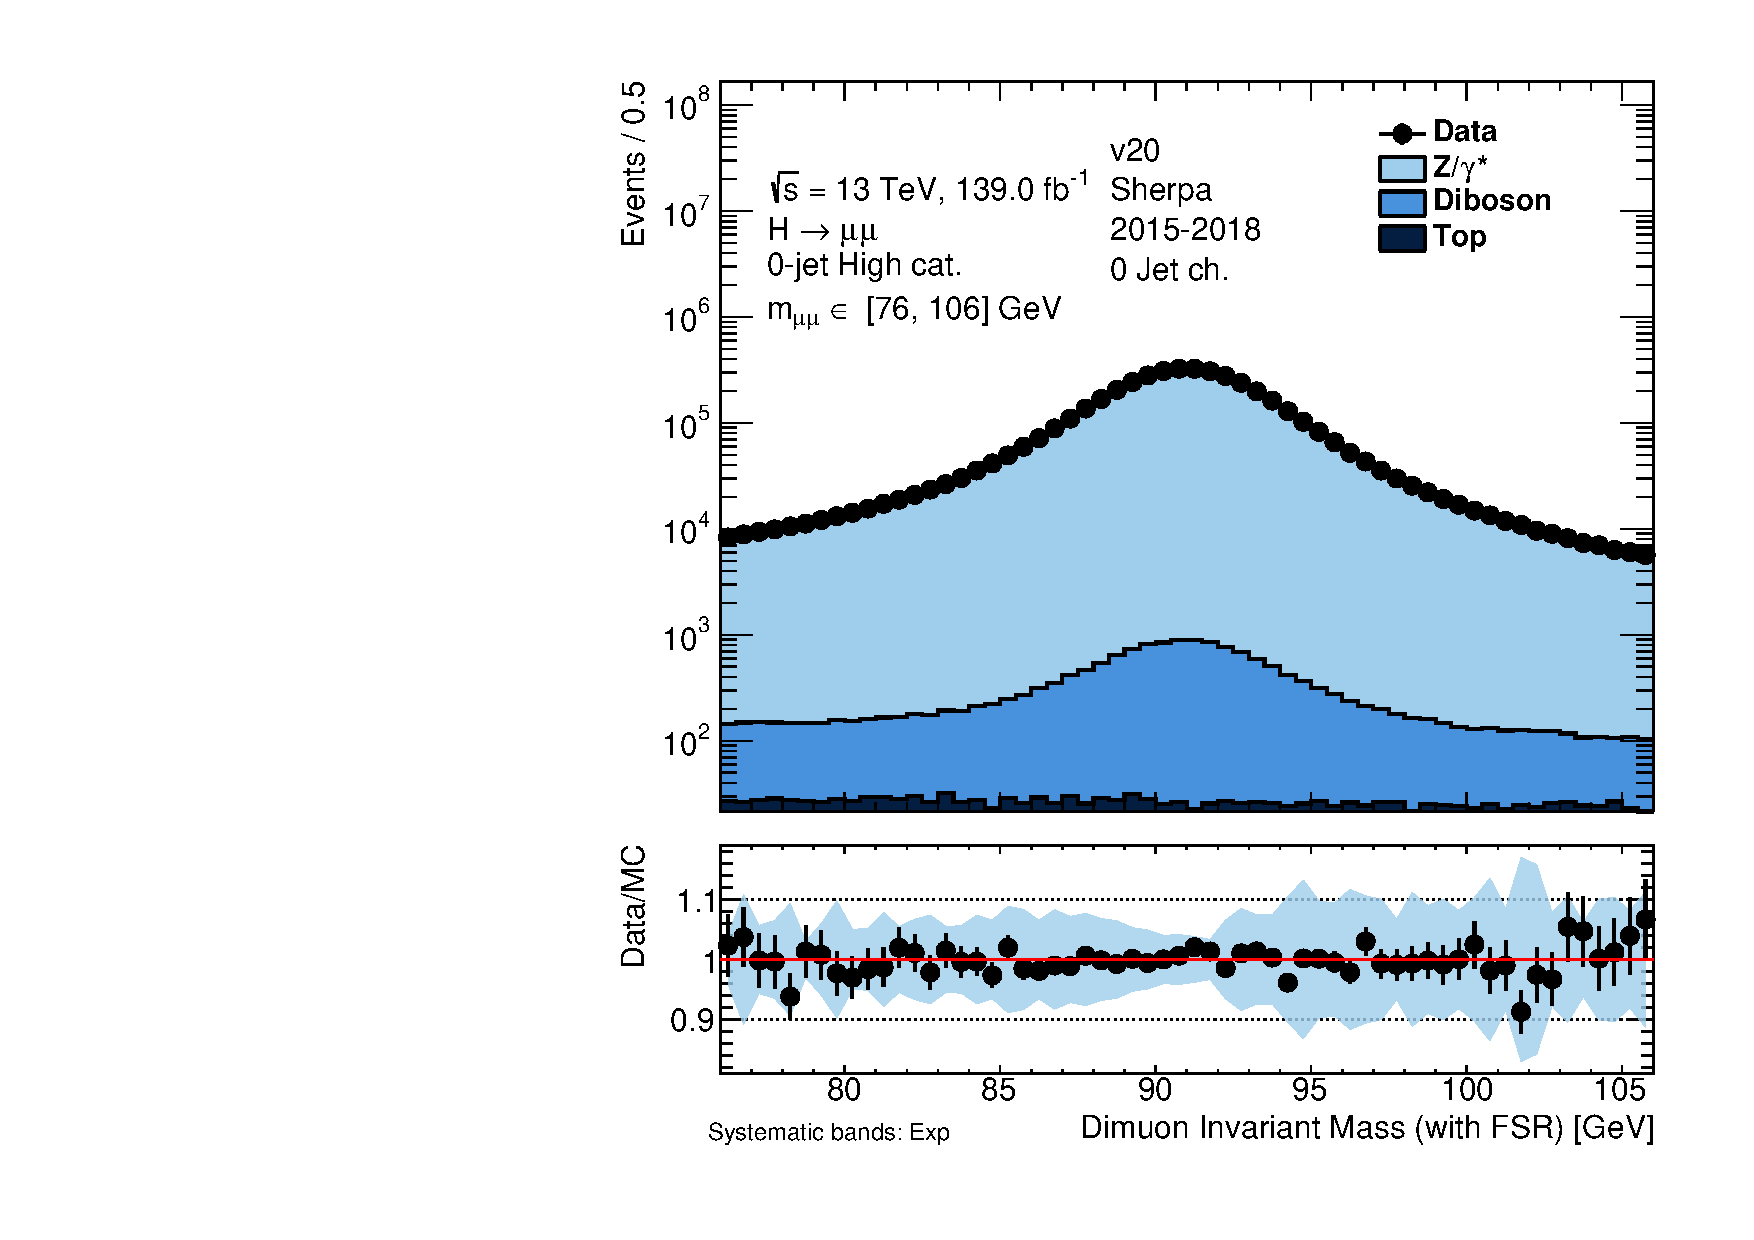
\includegraphics[width=0.49\textwidth]{figures/hmumu/reso/0jet_1}
  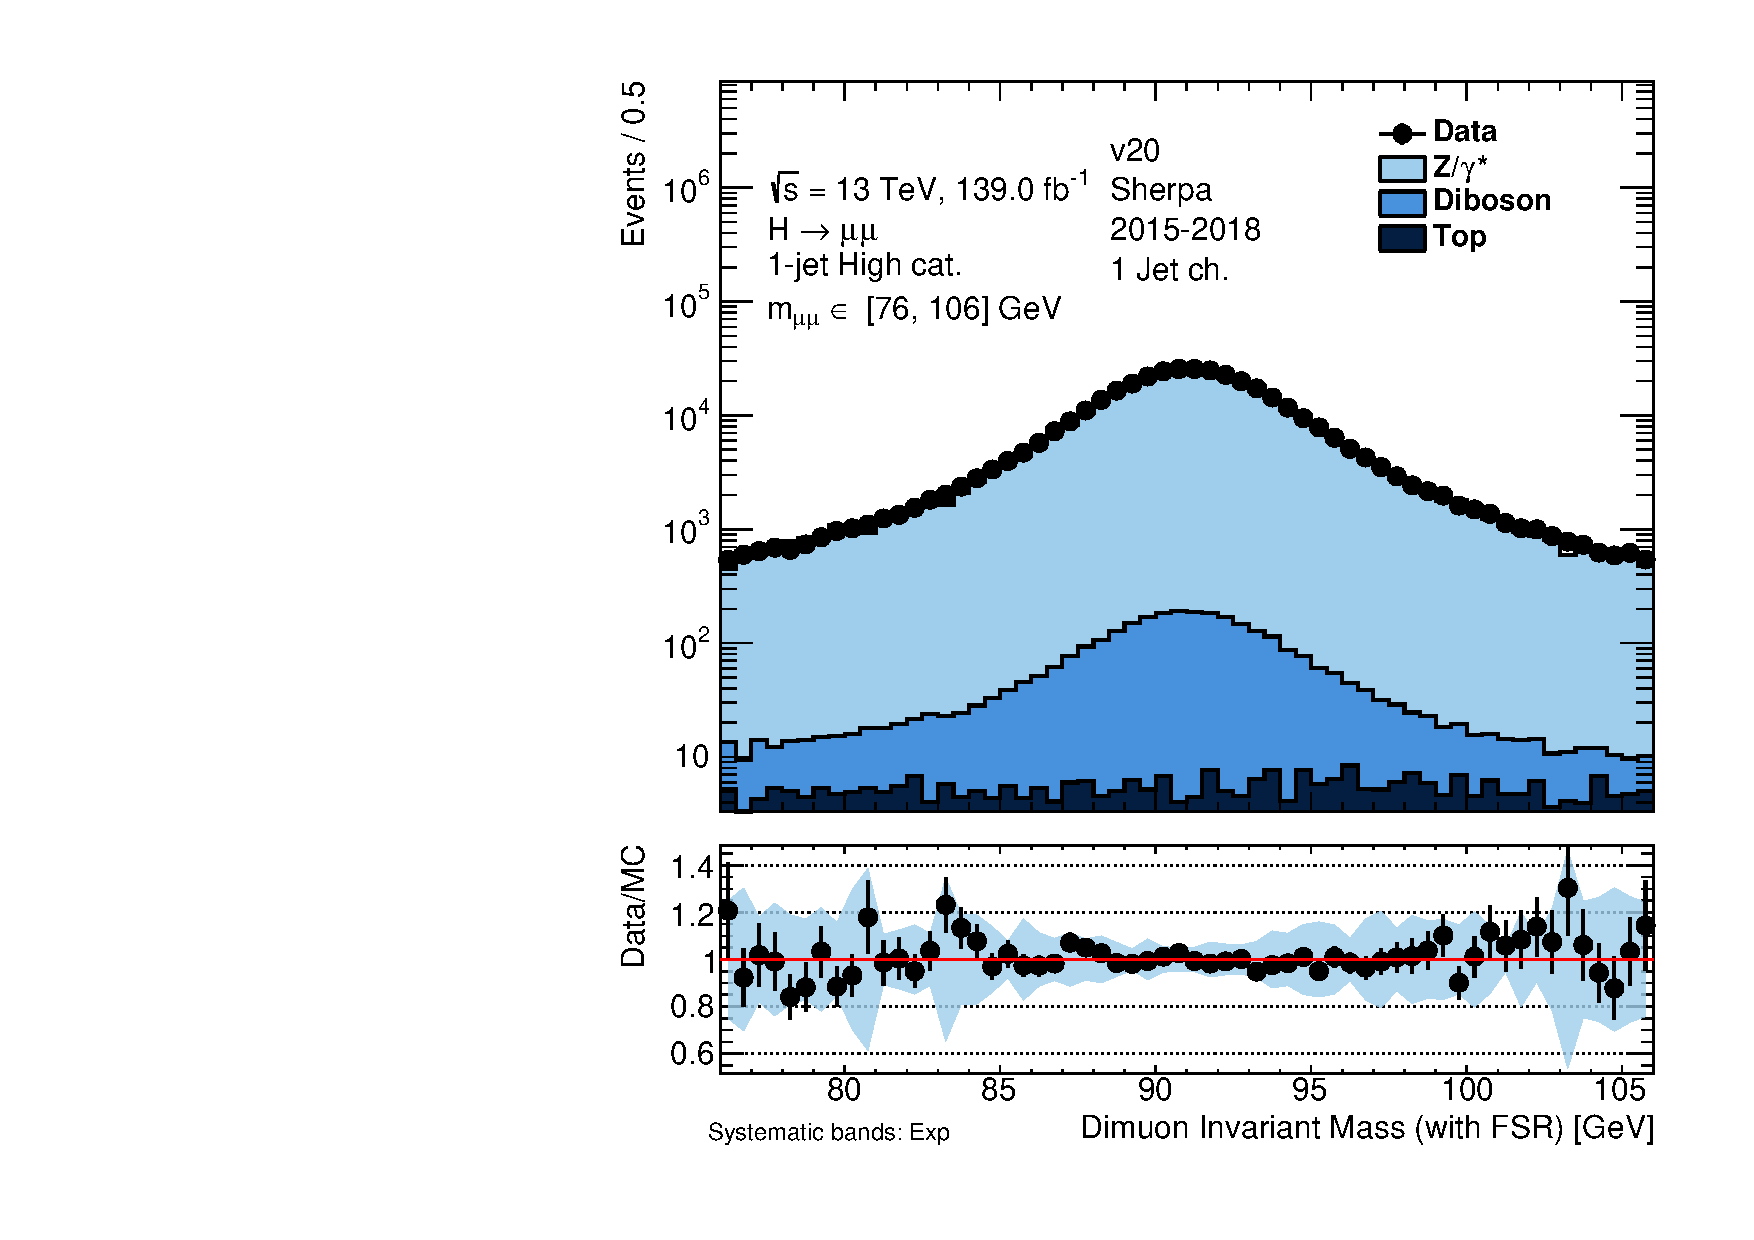
\includegraphics[width=0.49\textwidth]{figures/hmumu/reso/1jet_1}
  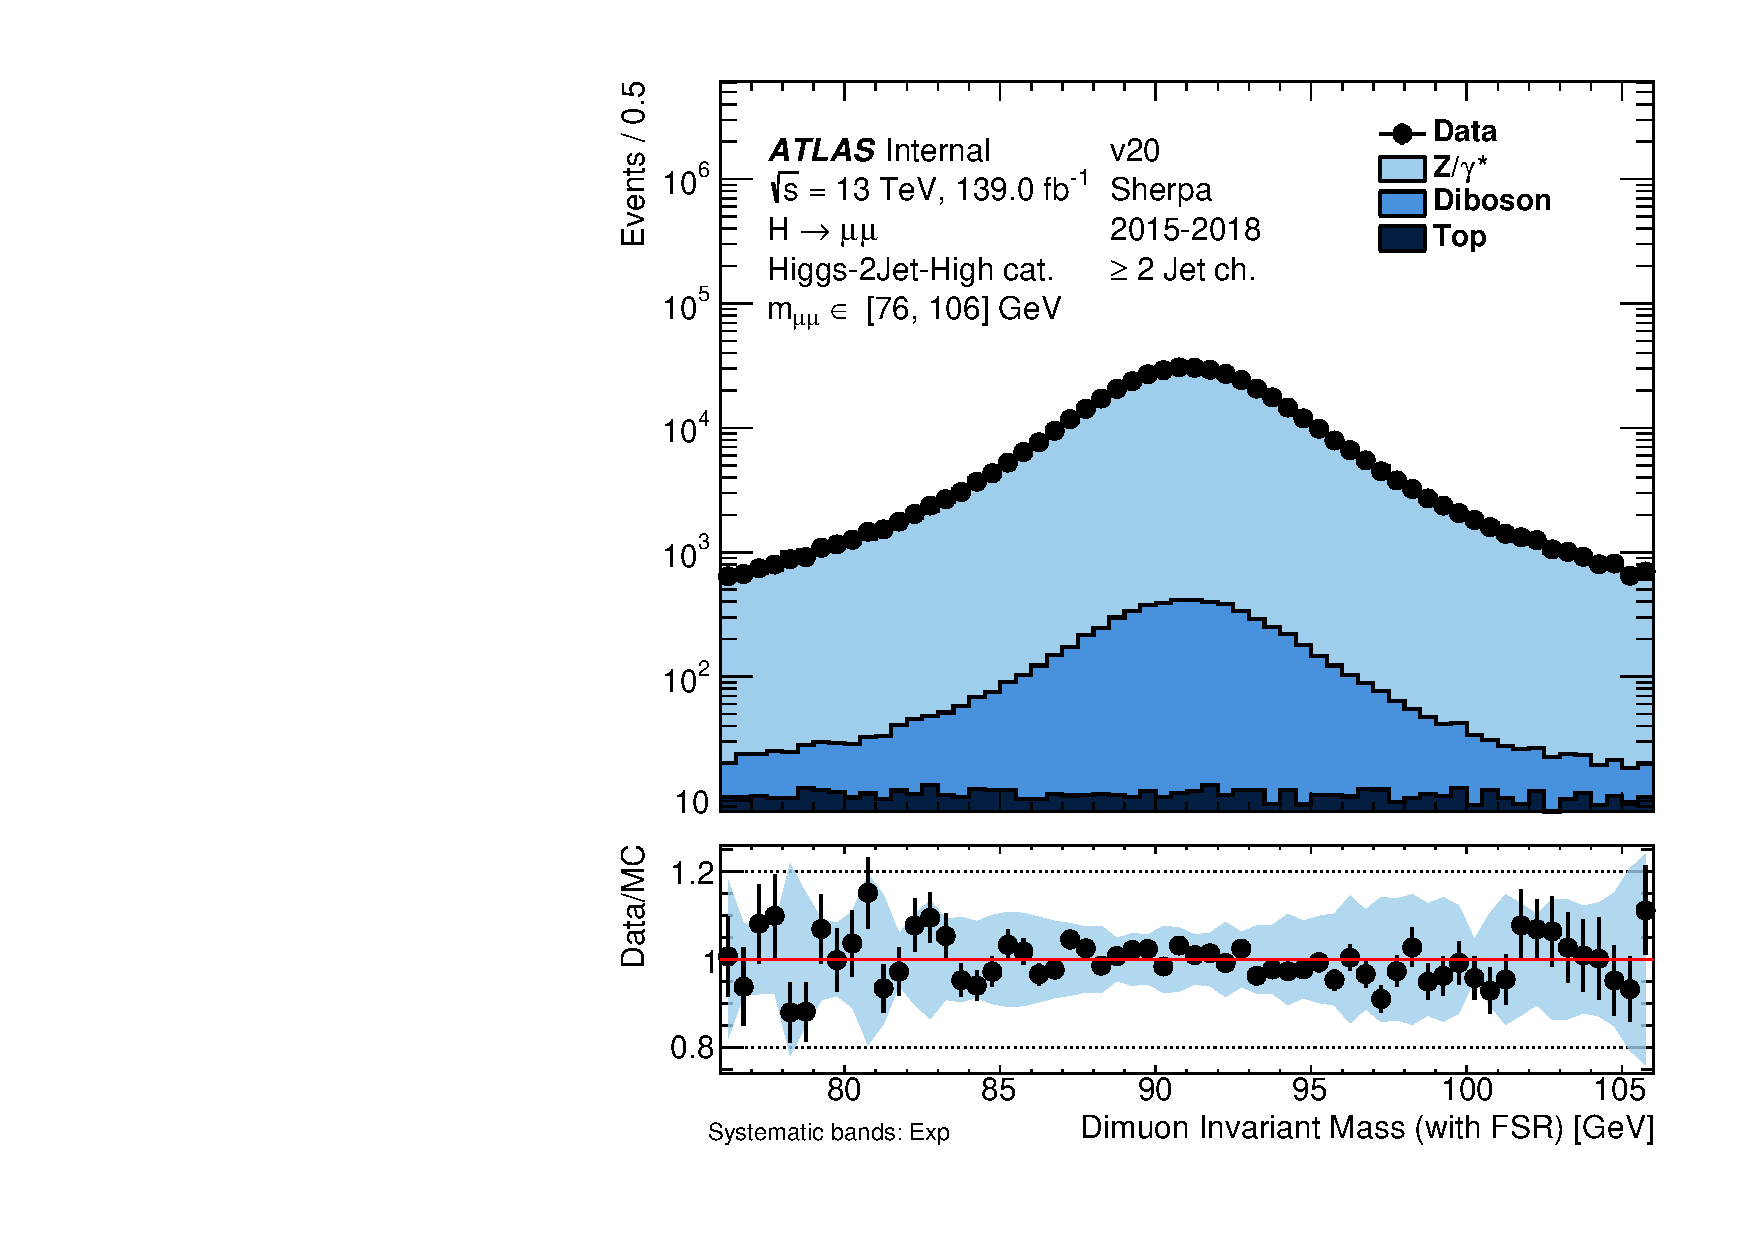
\includegraphics[width=0.49\textwidth]{figures/hmumu/reso/2jet_4}
  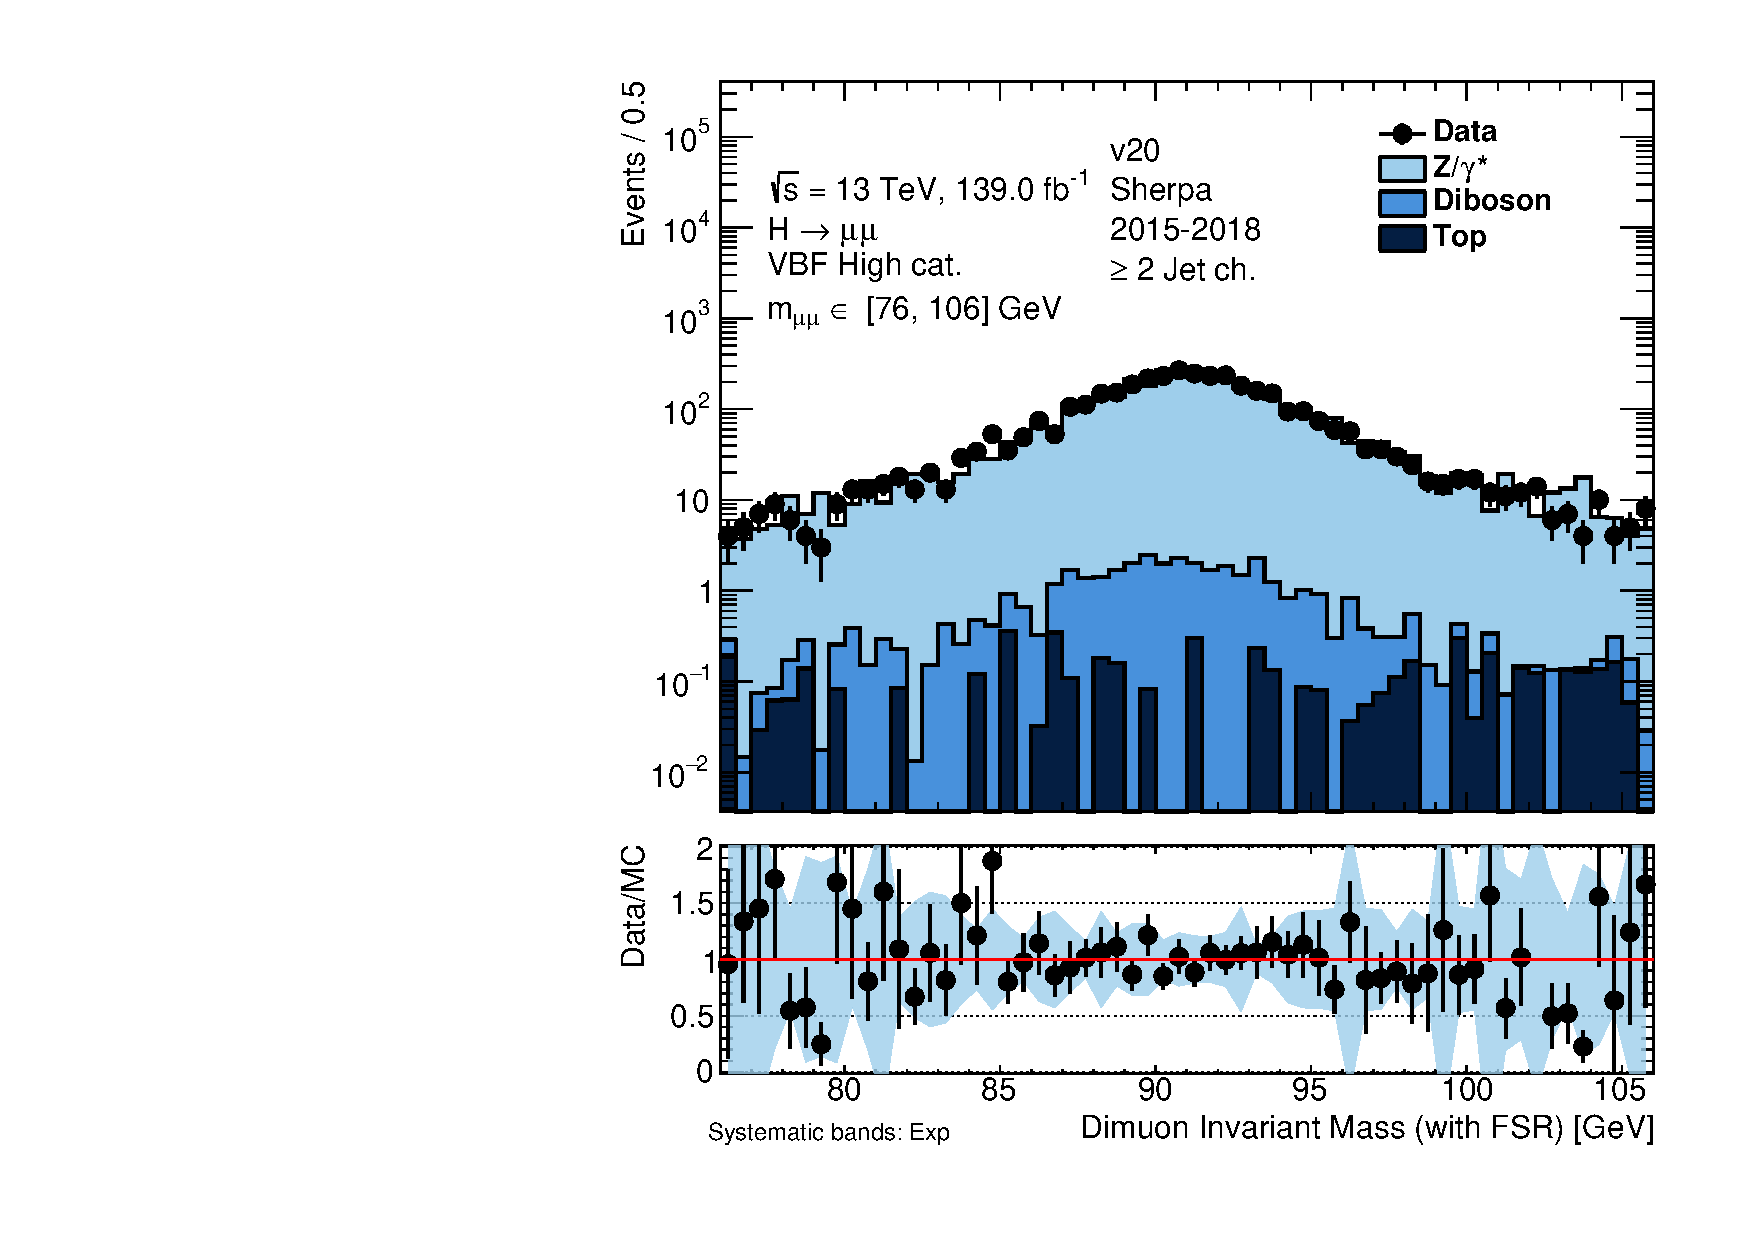
\includegraphics[width=0.49\textwidth]{figures/hmumu/reso/2jet_1}
  \caption[Mass resolution validation in analysis categories]{
  Invariant mass distribution after the FSR correction at the $Z$ peak
  for the 0-jet High, 1-jet High, 2-jet High, and VBF High
  analysis categories. Data is shown as black markers,
  Drell-Yan as light blue, diboson as blue, and top MC simulated events as
  dark blue histograms. MC simulation has been normalised to data
  for easier visual comparison. Bottom panel shows the ratio between data and
  MC simulation. Blue band represents experimental systematic
  uncertainties, while the black error bars represent combined
  statistical uncertainties on both data and MC simulation.
  }
  \label{fig:hmumu:reso}
\end{figure}

\section{Signal modelling}

The $\hmumu$ signal is modelled using an analytical function
with shape parameters determined from the maximum likelihood fit
to the MC simulation. In the combined signal and background fit
to data, shape parameters are kept fixed and only the normalisation
is adjusted to the data.

Since the analysis measures the signal strength multiplier,
defined with respect to the expected SM value, it is important
to evaluate the theoretical and experimental systematic
uncertainties which affect the signal normalisation.
Furthermore, since analysis sensitivity greatly depends on the
distribution of the signal among the different categories, the
systematic uncertainties which affect the kinematics of events,
not just their total normalisation, need to be evaluated.

\subsection{Signal parametrisation}

The Higgs boson has a width of only 4.1 \MeV, negligible compared
to the detector resolution of a few \GeV~in this momentum range.
As a result, the signal shape is dominated by detector resolution
effect and to some extent the quality of final state radiation
recovery.

It is modelled using a double-sided Crystal-Ball (DCSB) function
\cite{Oreglia:1980cs}, which has a Gaussian core
and tails on both sides, and is defined as \cite{Aaboud:2016tru}
\begin{equation}
\newcommand{\alow}{\alpha_\text{low}}
\newcommand{\ahigh}{\alpha_\text{high}}
\newcommand{\nlow}{n_\text{low}}
\newcommand{\nhigh}{n_\text{high}}
\newcommand{\for}{\text{for }}
    \text{DCSB} = N \cdot
    \begin{cases}
      e^{-\frac{1}{2}t^2}              &  \for -\alow \leq t \leq \ahigh \\
      e^{-\frac{1}{2}\alow^2} \left[ \frac{\alow}{\nlow} \left( \frac{\nlow}{\alow} -\alow - t \right) \right]^{-\nlow}  & \for t < -\alow \\
      e^{-\frac{1}{2}\ahigh^2} \left[ \frac{\ahigh}{\nhigh} \left( \frac{\nhigh}{\ahigh} -\ahigh + t \right) \right]^{-\nhigh}  & \for t > \ahigh,
    \end{cases}
\end{equation}
where $t = (\mmumu - \mu_\text{CB}) / \sigma_\text{CB}$, $N$ is the
normalisation constant, $\mu_\text{CB}$ and $\sigma_\text{CB}$ are
the mean and sigma of the central Gaussian distribution,
$\alpha_\text{low}$ ($\alpha_\text{high}$) parametrises the
invariant mass where the function transitions to the $n_\text{low}$
($n_\text{high}$) power law on the low-mass (high-mass) side of
the spectrum.

An alternative functional form, a sum of
a Gaussian and a one-sided Crystal-Ball has been tested with similar
results. Double-sided Crystal-Ball was chosen because its
parametrisation has a single mean and width and is more stable
during the fit.

The signal shape is obtained in each category separately by fitting
the combined signal from all main production modes. An alternative
approach, fitting production modes separately and combining them
in the proportions predicted by the SM, yielded very similar results
and was abandoned for simplicity.

The detailed form of the signal shape is expected to have little
impact on the result at the search stage. Nevertheless, injection
tests were carried out, fitting the functional form to a MC simulated
spectrum. The extracted signals matched the injection withing 0.5\%,
equal to the statistical precision of the test.

The fitted values of the $\mu_\text{CB}$ parameter were between
124.5 and 124.8 \GeV, while the $\sigma_\text{CB}$ parameter varied
between 2.5 and 3.0 \GeV~between the categories. Fitted DCSB models
are shown in Figure \ref{fig:hmumu:sig-model} for the VBF High and
0-jet High categories.
\begin{figure}[h!]
  \centering
  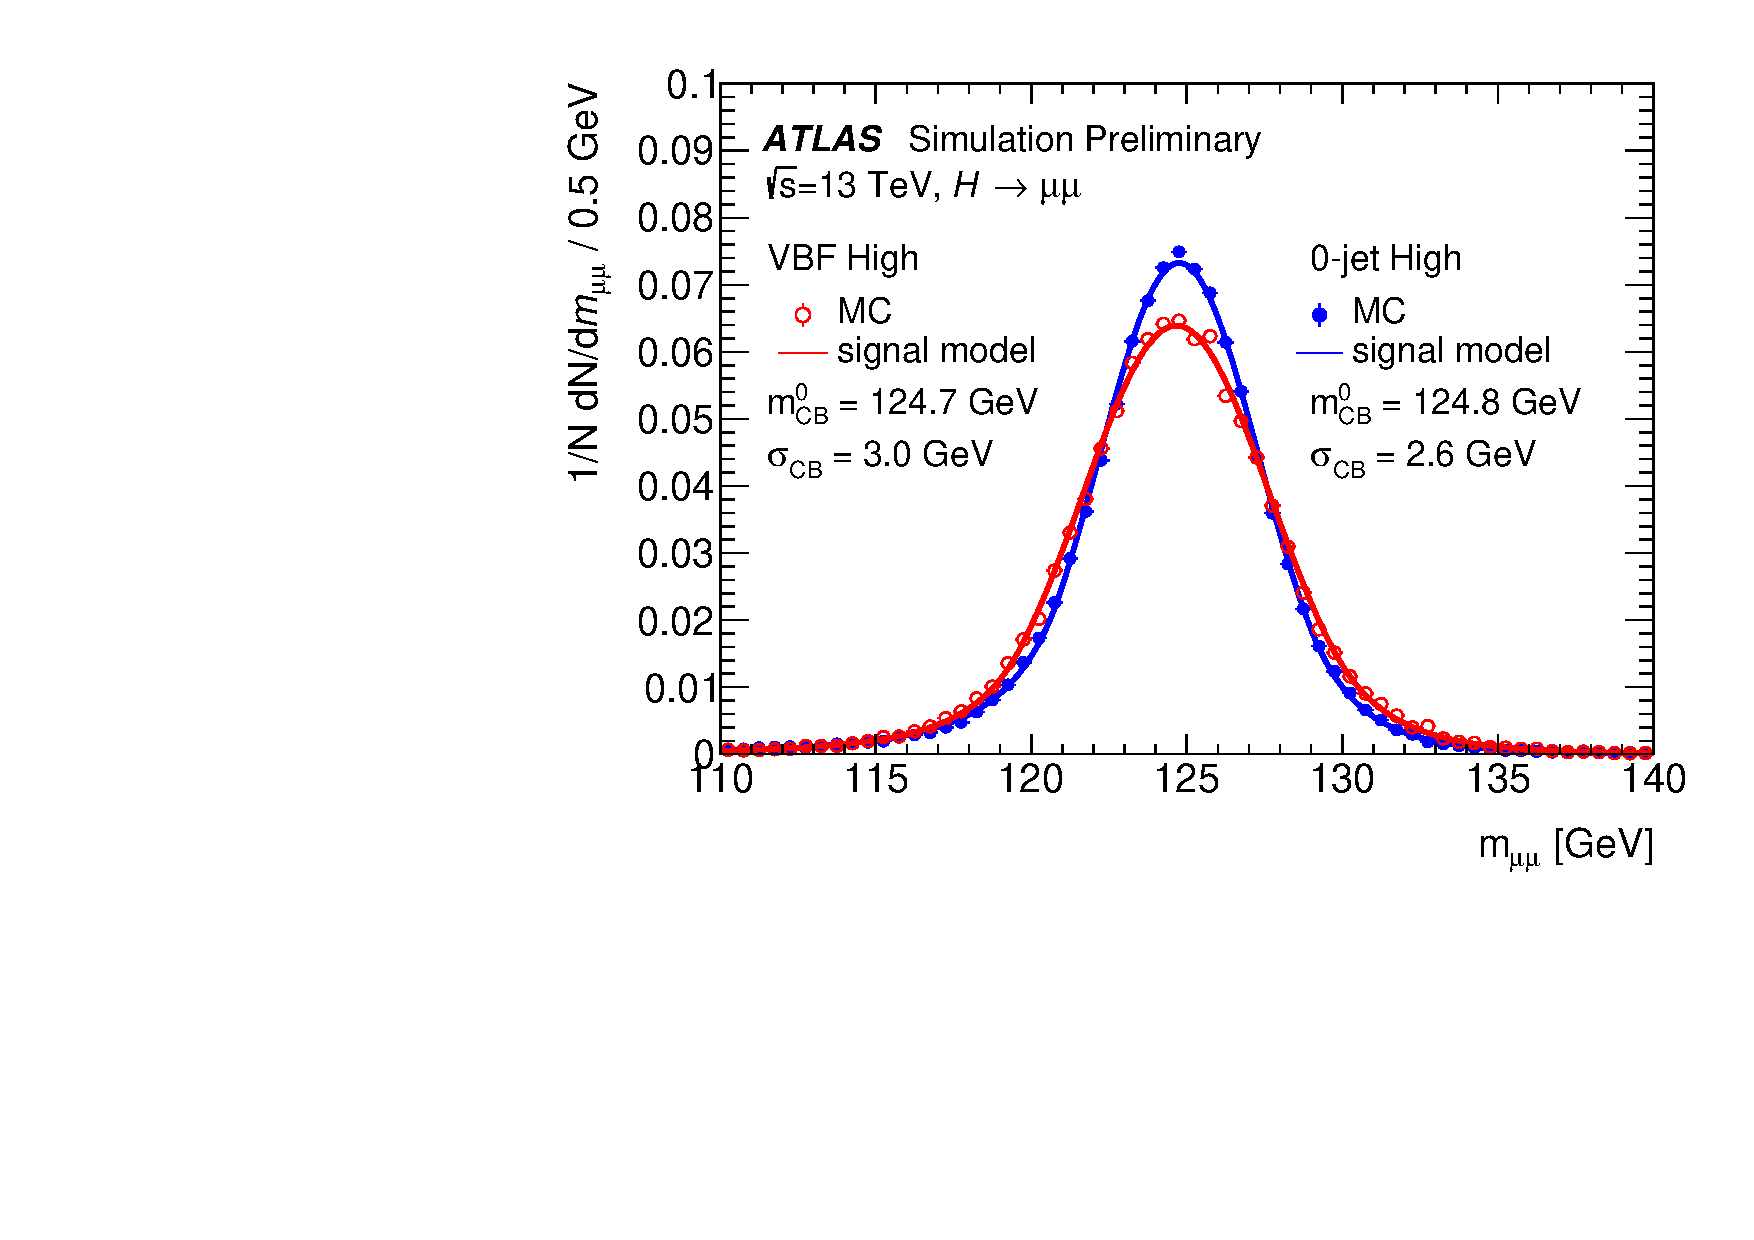
\includegraphics[width=0.8\textwidth]{figures/hmumu/sig-model}
  \caption[$\hmumu$ signal model]{
  DCSB signal model fit to the MC simulation of all Higgs production
  modes in the VBF High and 0-jet High analysis categories. VBF High
  category fit is shown as a red solid line, while the MC simulation
  is shown as empty red markers. The fit in the 0-jet High category
  is shown as a blue line, while the MC simulation is shown as solid 
  blue circles. The fitted values of $\mu_\text{CB}$ and
  $\sigma_\text{CB}$ parameters are shown on the left (right) side 
  for the VBF High (0-jet High) category. From Ref. \cite{ATLAS-CONF-2019-028}.
  }
  \label{fig:hmumu:sig-model}
\end{figure}

\subsection{Systematic uncertainties}

The signal normalisation and its distribution between the categories
are affected by both the theoretical and experimental systematic
uncertainties.

Theoretical uncertainties affecting the signal normalisation come from
the effect of missing higher order QCD corrections on the cross section
prediction, and the uncertainty on the branching ratio to muon pairs
\cite{deFlorian:2016spz}.

Some theoretical uncertainties also have an impact on the migration
of events between the categories, either because of the effect on the muon
or jet kinematics. These include the QCD scale variations, uncertainties
on the treatment of the underlying event and hadronisation, uncertainties
on the $\pt$ of the Higgs boson, uncertainties on migrations between
jet multiplicities and the treatment of top quark mass, following 
the prescription in Ref. \cite{deFlorian:2016spz}. The uncertainties
on the underlying event are evaluated by considering \textsc{Pythia} 8
eigentune variations and those on showering by considering events
showered by \textsc{Pythia} 8 and \textsc{Herwig} 7 \cite{Bahr:2008pv,
Bellm:2015jjp}. Dedicated uncertainties are also computed for the
acceptance of the $\ggf$ events in the VBF categories.

The individual size of theoretical uncertainties ranges between 
per mille level and 15\% for the $\ggf$ production mode,
while the uncertainties on the VBF production modes range
between per mille and level and 7\%.

Experimental systematic uncertainties affect the normalisation
and shape of the signal events as well as their distribution
between the categories.

For muons, the normalisation uncertainties come from the 
uncertainty in the scale factors for the reconstruction and
identification efficiencies, trigger, isolation selection, and
impact parameter efficiencies.

The only uncertainties which significantly alter the shape of the 
signal are the uncertainties on the muon scale and resolutions,
which affect the position and the width of the Higgs mass peak.

Systematic uncertainties on other objects used in the analysis
also have an effect on the analysis sensitivity, mainly by
affecting the distribution of signal events between the analysis
categories. In particular, $\met$ soft term uncertainties and 
uncertainties on the jet energy scale and resolution have an
important impact on the distribution of events in the VBF
categories in the 2-jet channel. Pile-up modelling has an
impact on migration of events between jet multiplicity channels,
while the uncertainties on the $b$-tagging efficiency affect
the number of events that pass the analysis selection.

Overall, the largest experimental uncertainty comes from the
jet energy scale and resolution, affecting signal yields in some
of the 2-jet categories by up to 10\%. The uncertainty from
the muon momentum resolution affects the fitted yields at the
1--6\% level, depending on the category.

Additionally, an uncertainty on the Higgs boson mass from Ref.
\cite{ATL-PHYS-PUB-2018-054, Aad:2015zhl} is found to have a
small impact. Finally, the uncertainty on the combined integrated
luminosity of the dataset at the level of 1.7\% is considered
\cite{ATLAS-CONF-2019-021, Aaboud:2016hhf}.


\section{Background modelling}

The very small signal to background ratio in the central region,
means that the modelling of the background is critical to the
success of the analysis. Since the number of background events
is much larger, a very small bias in the background model would
greatly impact the extracted signal.

The inclusive signal to background ratio is 0.2\% inclusively,
though this improves in some analysis categories. This requires
the control of the background shape to sub per mille level.

Analytical functions, motivated by the composition of the
background spectrum (dominated by DY, smaller contributions
from diboson and top), have been tried in the past but they have
struggled in particular to model the steeply falling spectrum
towards the $Z$ mass peak. In this analysis, a combination
of a rigid core and an empirical function is used instead.

The core function, common to all analysis categories and without
free parameters, models the steep part of the spectrum. The
empirical function models the differences in categories
due to selection and resolution effects, and is selected
using the custom DY dataset, described in Section \ref{sec:hmumu:customDY}.
The value of the spurious signal uncertainty is extracted
simultaneously.

\subsection{Background parametrisation}

The background model is constructed in each analysis category
separately, by multiplying a common core function with an
empirical function specific to the category,
\begin{equation}
F(\mmumu) = F_\text{core}(\mmumu) \cdot F_{\text{empirical}}(\mmumu).
\end{equation}

The core function describes the inclusive DY spectrum and
is able to model the steeply falling part of the spectrum.
It is constructed from the analytic LO Drell-Yan line-shape
\cite{Aaboud:2017ffb}, convolved by the normal distribution
with width parametrised as a function of $\mmumu$ to model
the effects of detector resolution,
\begin{equation}
F_\text{core}(\mmumu) =
\left( \sum_q \mathcal{L}_{q\bar q}(\mmumu) \cdot \sigma_{q\bar q}(\mmumu) \right) * \mathcal{N}(0, \sigma(\mmumu)),
\end{equation}
where the sum over $q$ runs over the lightest three quarks,
$q = u, s, d$, the parton luminosity component $\mathcal{L}_{q\bar q}$
is derived using PDF4LHC15 PDF for the LO using APFEL
\cite{Bertone:2013vaa} and LHAPDF \cite{Buckley:2014ana}.
The cross-section component
$\sigma_{q\bar q}(\hat s) = \sigma_{q\bar q}(\mmumu) / (2\mmumu)$
can be written as \cite{ATLAS-CONF-2019-028}
\begin{equation}
\sigma_{q\bar q}(\hat s) = \frac{4\pi \alpha^2}{3\hat s N_c}
\left[
Q_q^2 - 2 Q_q V_\ell V_q \chi_{Z\gamma} (\hat s) +
(A_\ell^2 + V_\ell^2) (A_q^2 + V_q^2) \chi_Z(\hat s)
\right],
\end{equation}
where
\begin{align}
 \chi_{Z\gamma}(\hat s) & = \kappa \frac{\hat s (\hat s - m_Z^2)}{(\hat s - m_Z^2)^2 + \Gamma_Z^2 m_Z^2}, \\
 \chi_{Z}(\hat s)       & = \kappa^2 \frac{{\hat s}^2}{(\hat s - m_Z^2)^2 + \Gamma_Z^2 m_Z^2}, \\
 \kappa                 & = \frac{\sqrt{2}G_Fm_Z^2}{4\pi \alpha},
\end{align}
and $\hat s = \mmumu^2$, $Q_q$ is the electric charges of the quarks,
$V_f$ and $A_f$ are the vector and axial vector couplings of the fermions,
$\alpha$, $G_F$ are the electroweak couplings,
$m_Z$ and $\Gamma_Z$ are the mass and the width of the $Z$ boson with values
taken from Ref. \cite{Patrignani:2016xqp},
and $N_c = 3$ is the number of colour charges.

The resolution function $\sigma(\mmumu)$ is derived from the
MC simulation of Drell-Yan samples, simulated by Sherpa,
by comparing the truth and reconstructed invariant mass.

The empirical function is chosen among two families of functions,
namely ``PowerN",
\begin{equation}
\text{PowerN}(\mmumu) = \mmumu^{(a_0 + a_1\mmumu + a_2 \mmumu^2 + ... + a_N\mmumu^N)},
\end{equation}
and ``EpolyN",
\begin{equation}
\text{EpolyN}(\mmumu) = e^{(a_1\mmumu + a_2 \mmumu^2 + ... + a_N\mmumu^N)},
\end{equation}
where $a_n$ are the free parameters, according to the selection
procedure outlined in Section \ref{sec:hmumu:model-sel}.

\subsection{Model selection}
\label{sec:hmumu:model-sel}

The empirical function is chosen separately in each analysis
category, by first reducing the set of functions to those
satisfying the following criteria:
\begin{itemize}
\item $\chi^2$ probability of the background-only fit must
be larger than 1\% for:
\begin{itemize}
\item data in the fit region (excluding the $120-130$ \GeV),
\item ATLAS MC simulation of DY, diboson, and top backgrounds in the fit region,
\item custom DY sample, reweighted to the data sidebands using a second order polynomial.
\end{itemize}
\item Pass the spurious signal test, defined in Section \ref{sec:hmumu:sstest},
i.e. require the $\text{SS} < 20\%~\delta$S, where SS is the fitted signal
yield (the spurious signal), and $\delta$S is the statistical uncertainty
on the signal strength obtained from the data corresponsing to 139 $\ifb$.
\item If multiple functions pass the first two criteria,
the function(s) with the fewest number of free parameters is (are)
chosen.
\item If more than one function remains, the function with the
smallest value of SS is chosen.
\end{itemize}
The selected functions are shown in Table \ref{tab:hmumu:ss}
for each of the analysis categories. The spurious signal uncertainty
is considered as uncorrelated across the categories, since none
of the values are more than two standard deviations away from zero,
when considering the statistical uncertainty on the custom DY sample,
corresponding to approximately 700 times the statistics of the
dataset.
\begin{table}[htb]
  \centering
  \caption{
    Selected empirical function components of the background model
    in each of the analysis categories. Also shown are the SS values,
    defined as the maximum of the fitted signals in the 120--130
    \GeV~mass range, normalised to the expected statistical error
    on the fitted signal ($\delta$S and to the SM predictions
    for signal yields in the analysis categories (S$_\text{SM}$).
    Reproduced from Ref. \cite{ATLAS-CONF-2019-028}.}
  \label{tab:hmumu:ss}
  \begin{tabular}{cccc}
    \toprule
    Category & Empirical Function & max(SS/$\delta$S)[\%] & max(SS/S$_{SM}$)[\%] \\
    \midrule
    VBF High & Power0 & 10.6 & 14.7 \\
    VBF Medium & Epoly2 & 0.51 & 1.3 \\
    VBF Low & Power1 & 3.6 & 7.5 \\
    2-jet High & Epoly2 & 8.7 & 16.3 \\
    2-jet Medium & Epoly4 & 1.2 & 3.9 \\
    2-jet Low & Epoly3 & -8.2 & -33.2 \\
    1-jet High & Power1 & 6.1 & 12.1 \\
    1-jet Medium & Epoly3 & -8.1 & -19.8 \\
    1-jet Low & Epoly3 & -2.5 & -5.8 \\
    0-jet High & Power1 & 14.6 & 26.5 \\
    0-jet Medium & Epoly3 & -11.6 & -39.0 \\
    0-jet Low & Epoly3 & -18.5 & -74.2 \\
    \bottomrule
  \end{tabular}
\end{table}

\subsection{Spurious signal uncertainty}
\label{sec:hmumu:sstest}

The spurious signal value is determined by a combined signal
and background model fit to the invariant mass spectrum
in the fit region of the custom DY sample, shown in Figure
\ref{fig:hmumu:ss}. Prior to the fit,
the DY sample is re-weighted to the data sidebands using a first
order polynomial in the VBF categories, and a second order
polynomial in the other categories. The re-weighting mitigates
the potential mismodelling of the invariant mass shape by the
MC simulation.

\begin{figure}[h!]
  \centering
  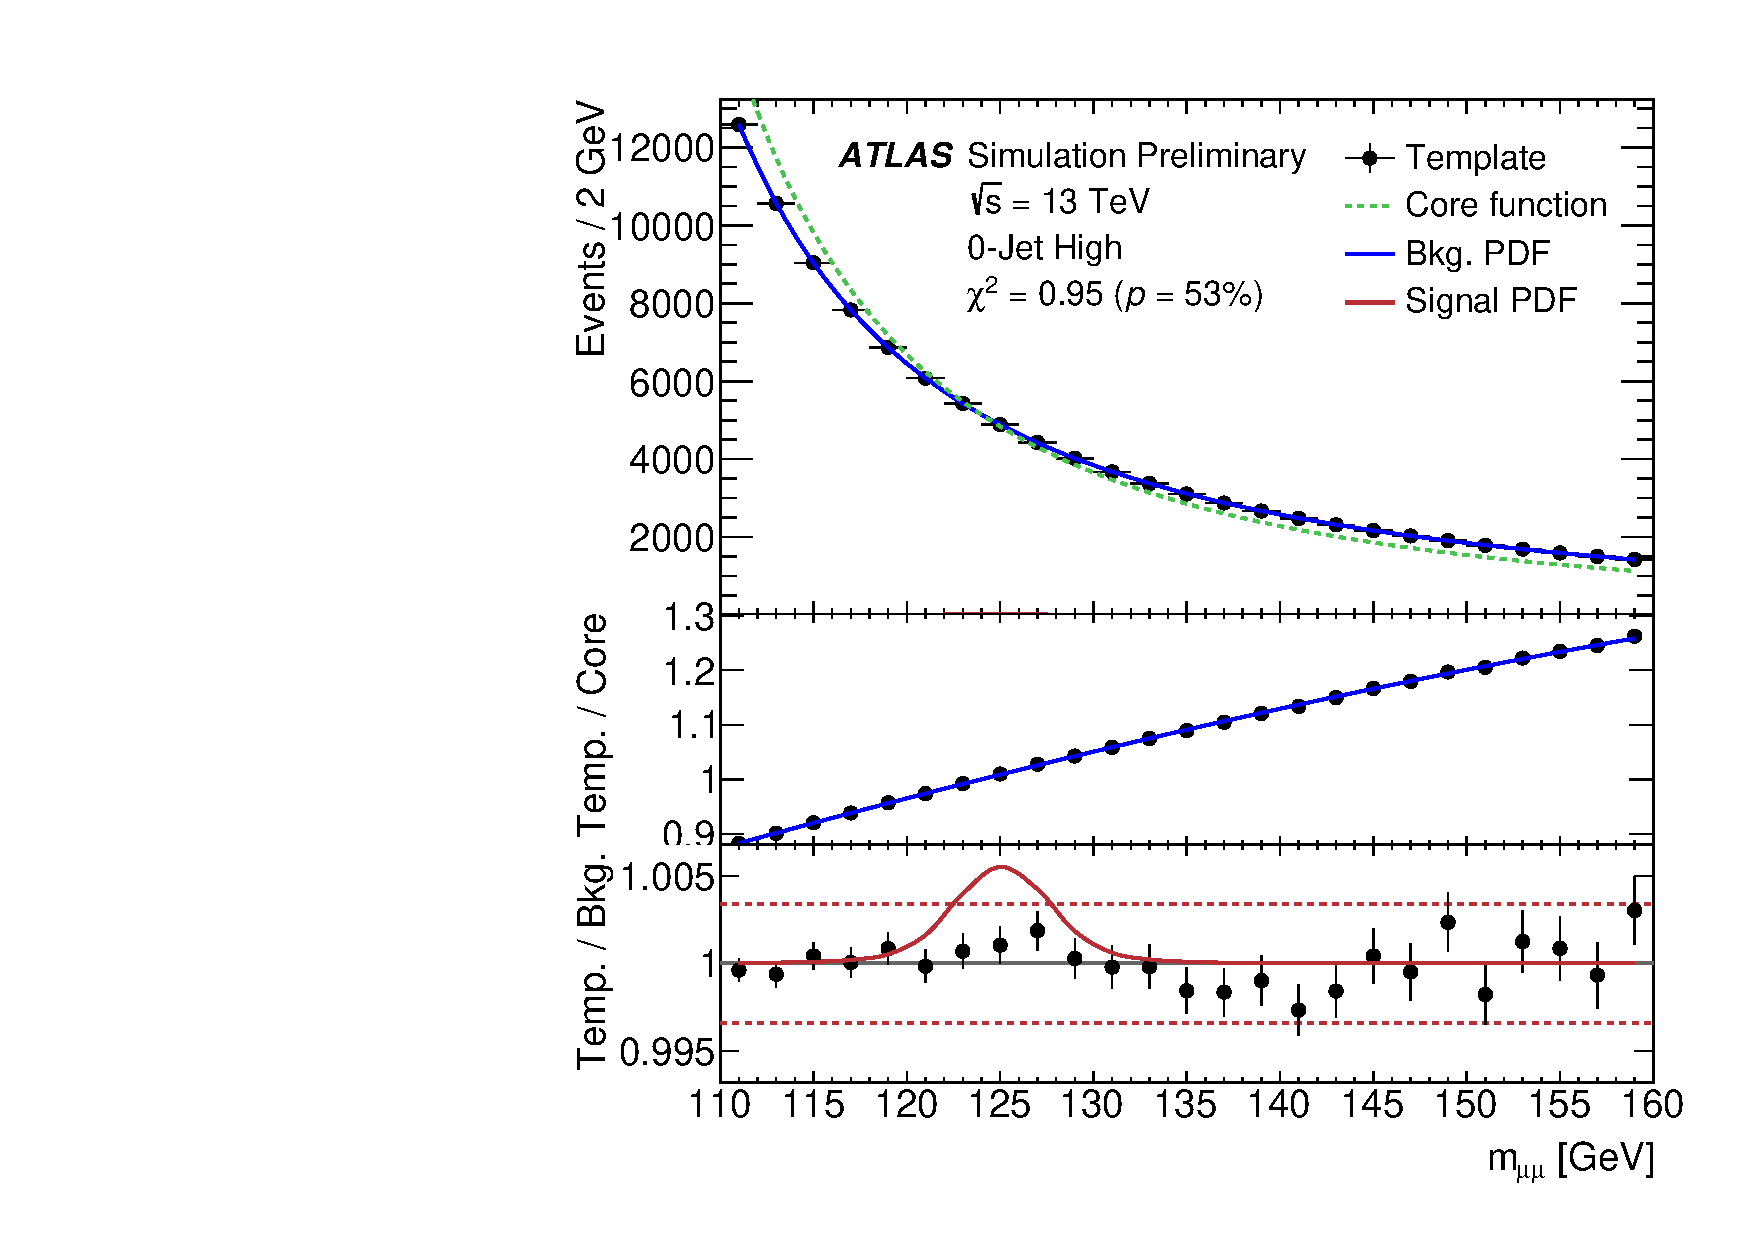
\includegraphics[width=0.47\textwidth]{figures/hmumu/SS/BDT10}
  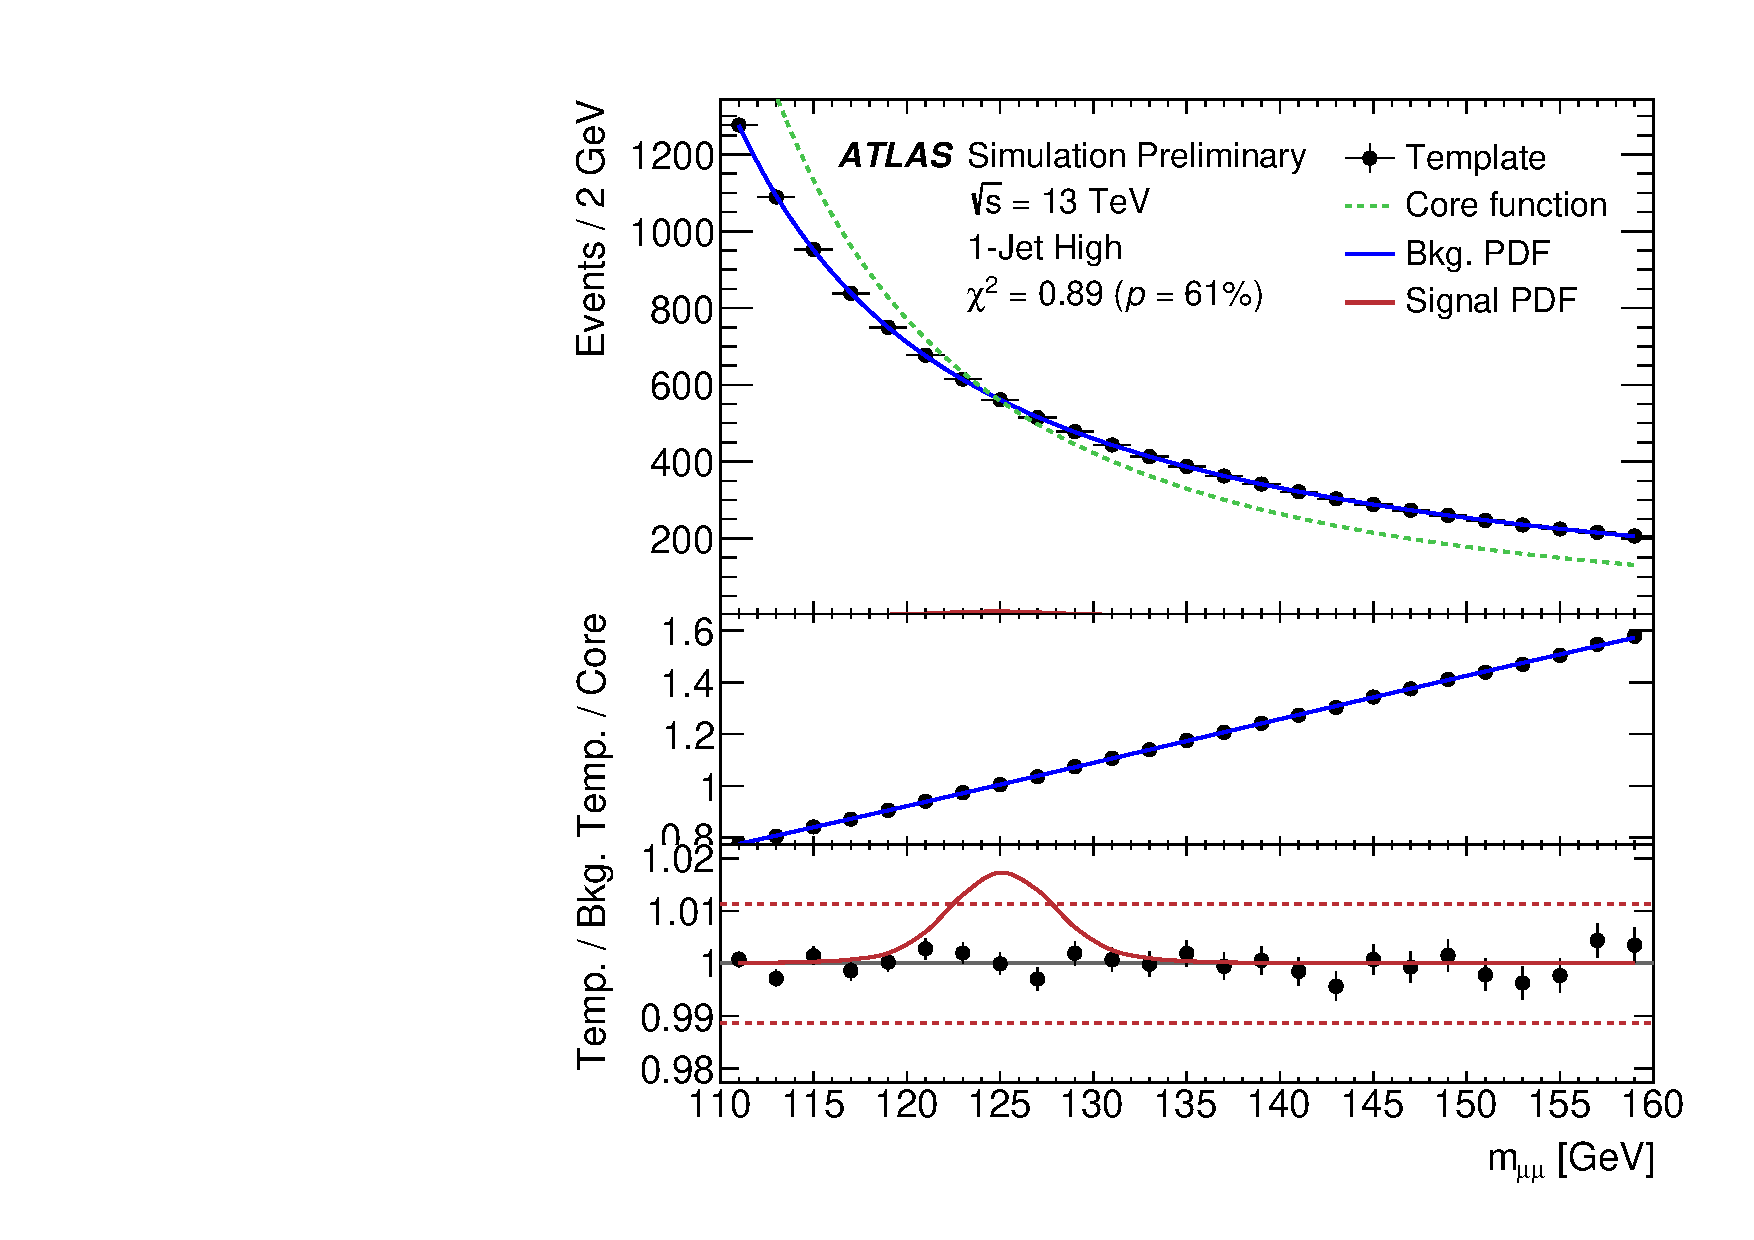
\includegraphics[width=0.47\textwidth]{figures/hmumu/SS/BDT7}
  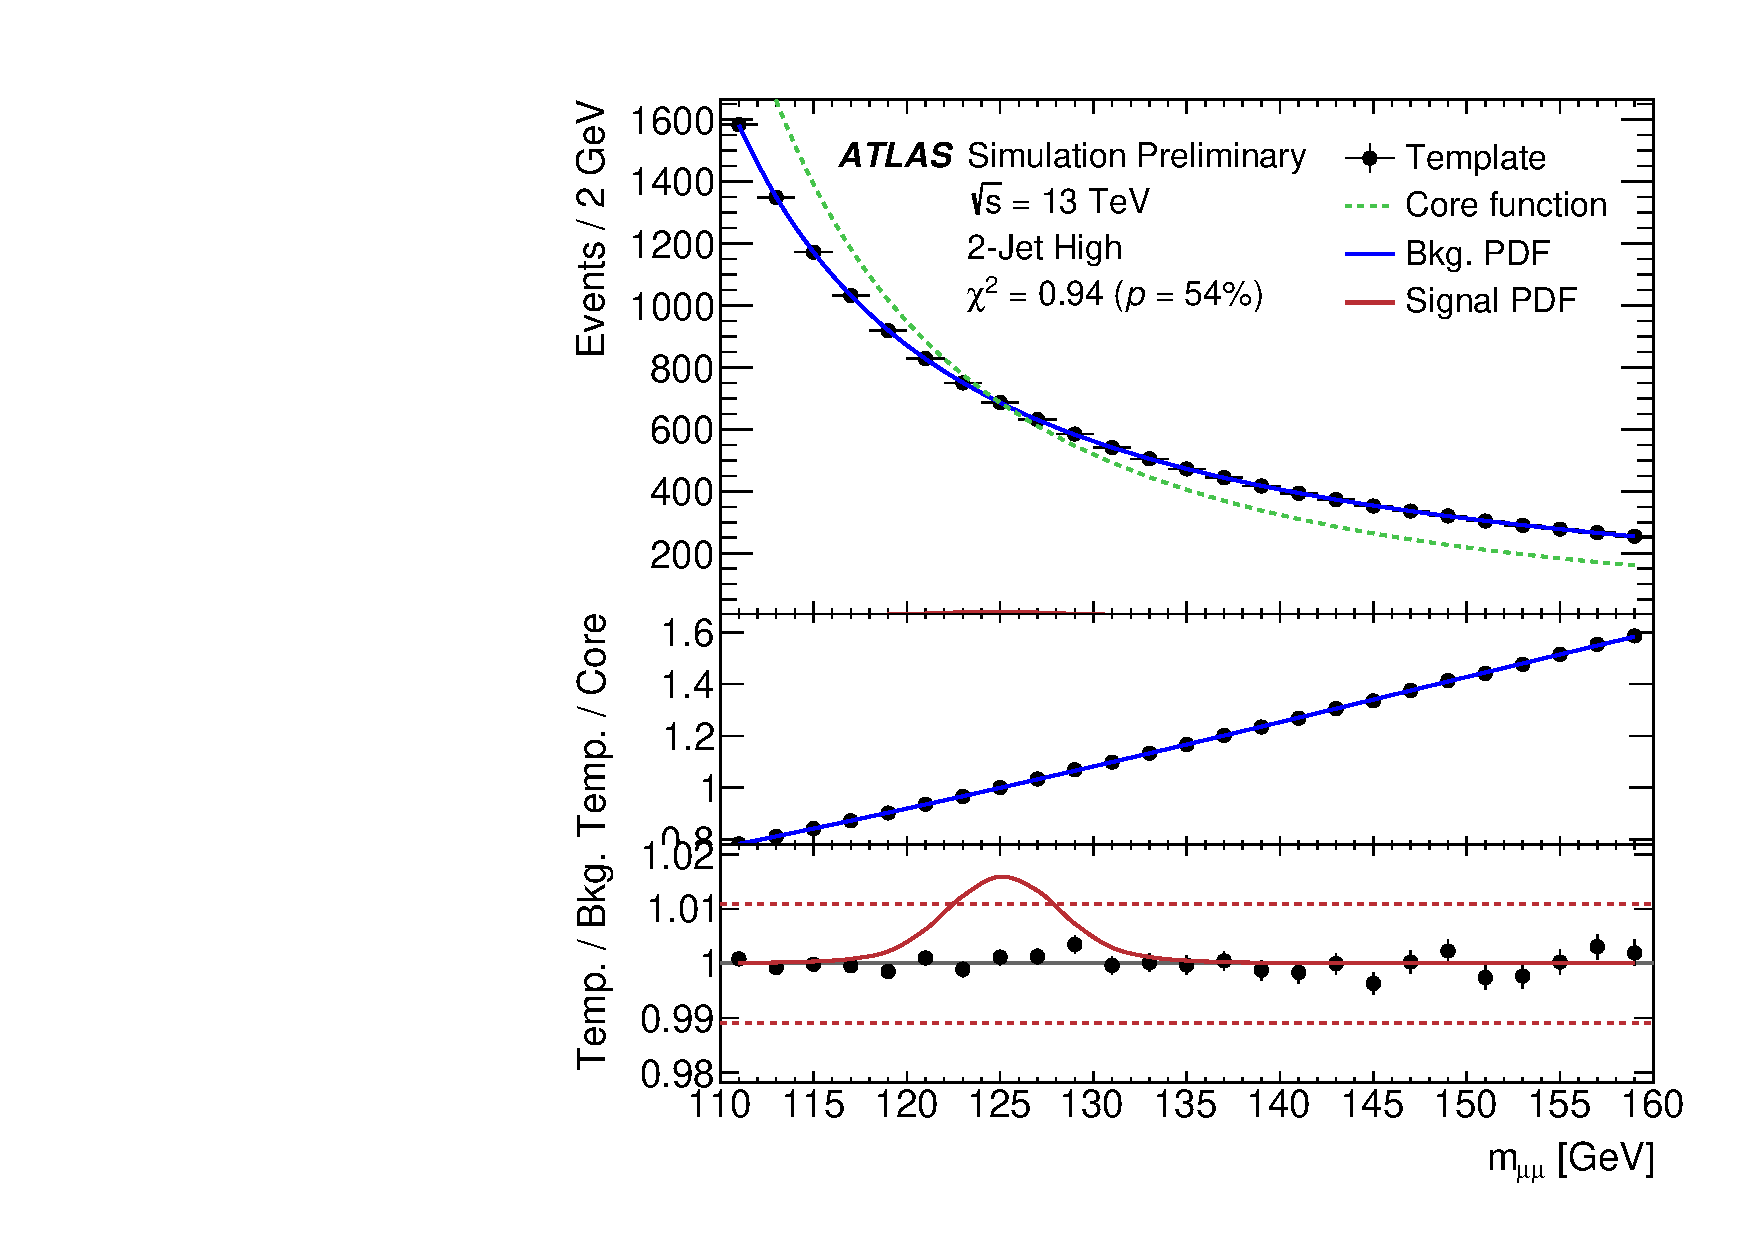
\includegraphics[width=0.47\textwidth]{figures/hmumu/SS/BDT4}
  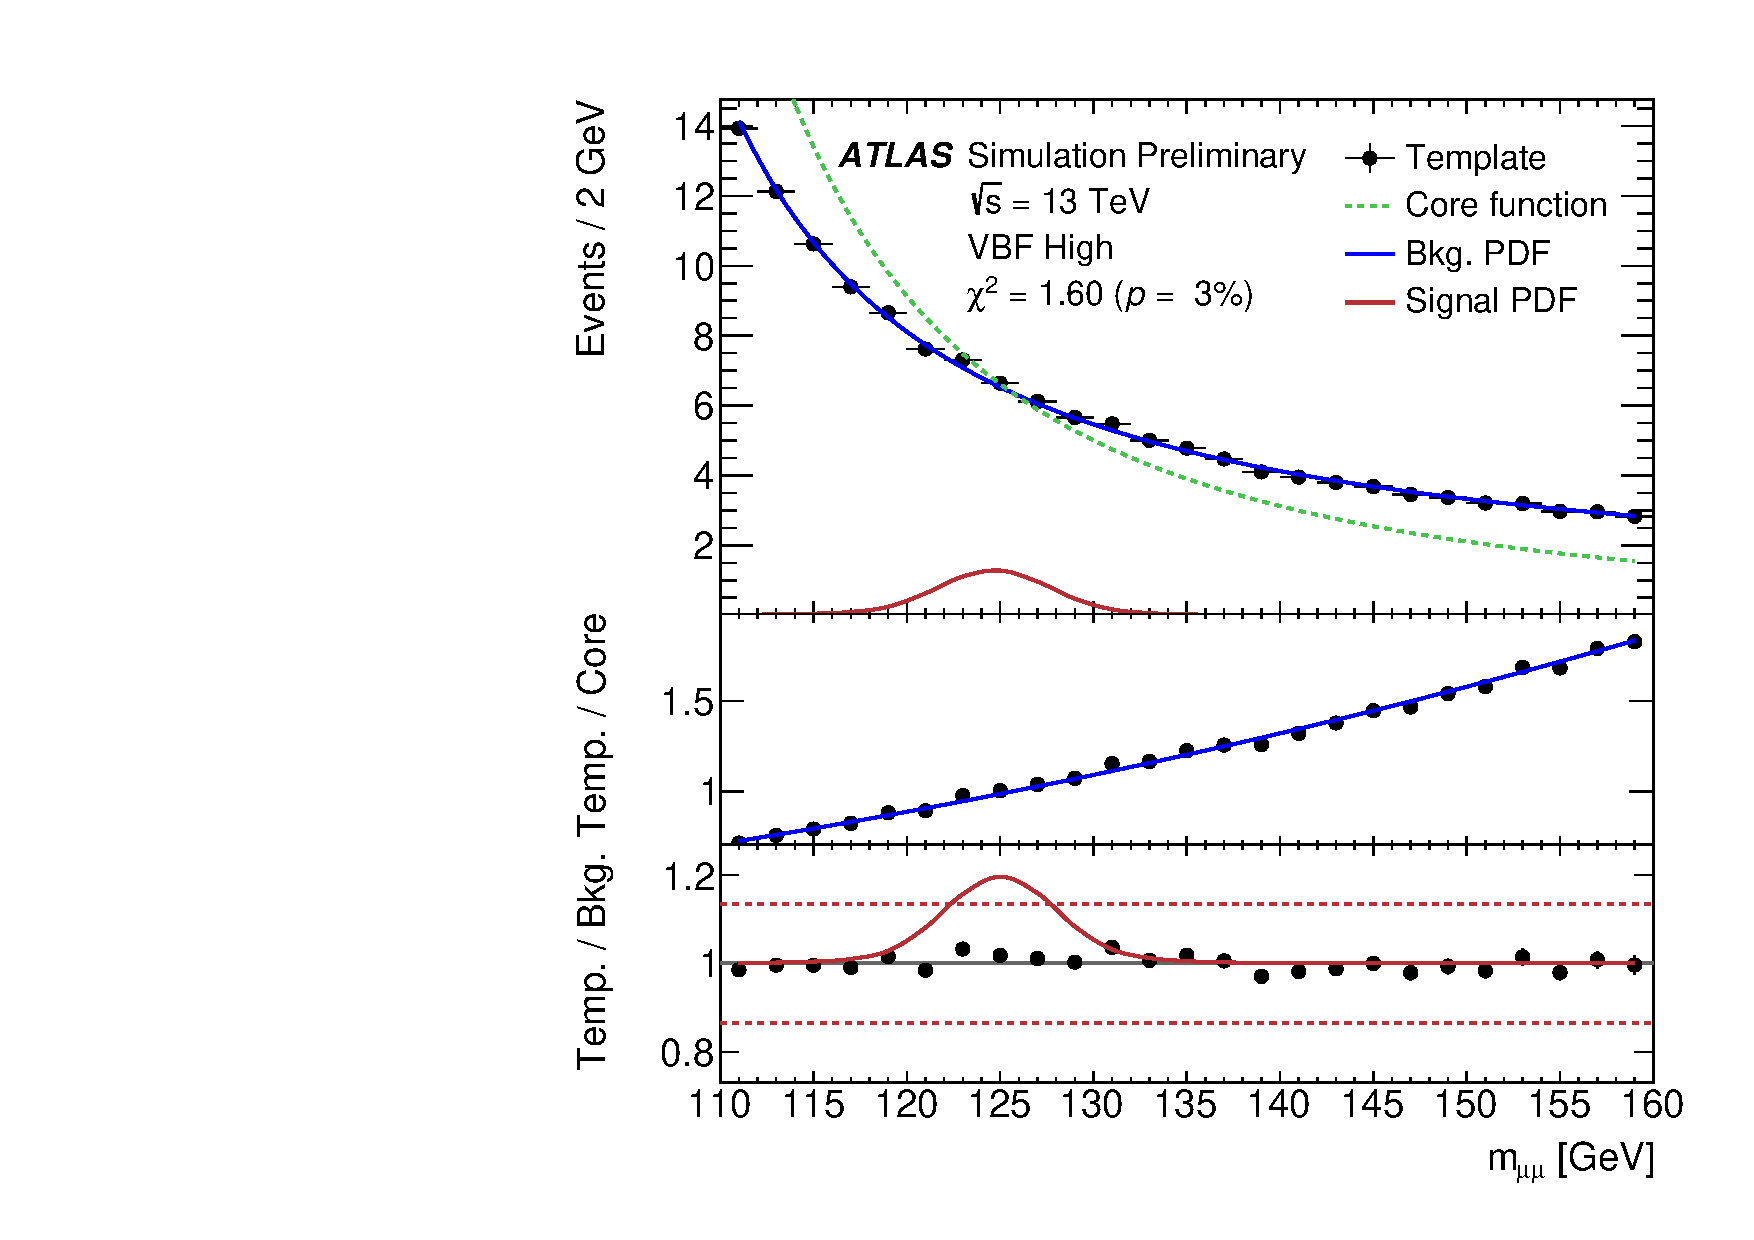
\includegraphics[width=0.47\textwidth]{figures/hmumu/SS/BDT1}
  \caption[Spurious signal fit to custom DY mass spectrum]{
  Combined signal and background fit to the custom DY invariant
  mass spectrum in 0-jet High, 1-jet High, 2-jet High, and VBF-high
  analysis categories. The top panel shows the custom DY template
  as black points, fixed core function as a dashed green line,
  and the full background model as a solid blue line. Signal shape,
  normalised to the SM prediction, is shown as a red line.
  Reduced $\chi^2$ value of the fit and the corresponding
  $\chi^2$-probability are also shown. The middle panel shows
  the the custom DY template, divided by the core function (black
  points) and the empirical function (blue solid line). The bottom
  panel shows the ratio between the custom DY template and
  full background model as black points. Signal shape, divided
  by the background model is shown as a solid red line. The dashed
  red lines in the bottom panel denote the expected signal purity
  in the central region. From Ref. \cite{ATLAS-CONF-2019-028}.
  }
  \label{fig:hmumu:ss}
\end{figure}

A number of scans is performed, varying the signal mass parameter
between 120 and 130 \GeV~in 1 \GeV~steps, while the other parameters
of the signal model are kept to the values obtained in the fit.
The maximum value of the fitted signal across this range is taken
as the total spurious signal SS.

The sensitivity of the SS value to the shape of the custom DY
spectrum was evaluated by fitting the combined signal and
background model to the systematic variations of custom DY
spectrum. For theoretical systematic uncertainties, the variations
of the QCD renormalisation scale and using alternative PDF sets
were considered. From the experimental side, the systematic
variations of muon momentum scale and resolution in the ID and
MS detectors were used. The obtained SS values from the
systematic variations were not significantly different from
those obtained from the nominal template.

It should be noted that the custom DY samples are only used in
selecting the empirical part of the function and the evaluation
of the spurious signal systematic uncertainty. They are not used
at all when fitting the invariant mass spectum in data.

\section{Results}


\begin{figure}[h!]
  \centering
  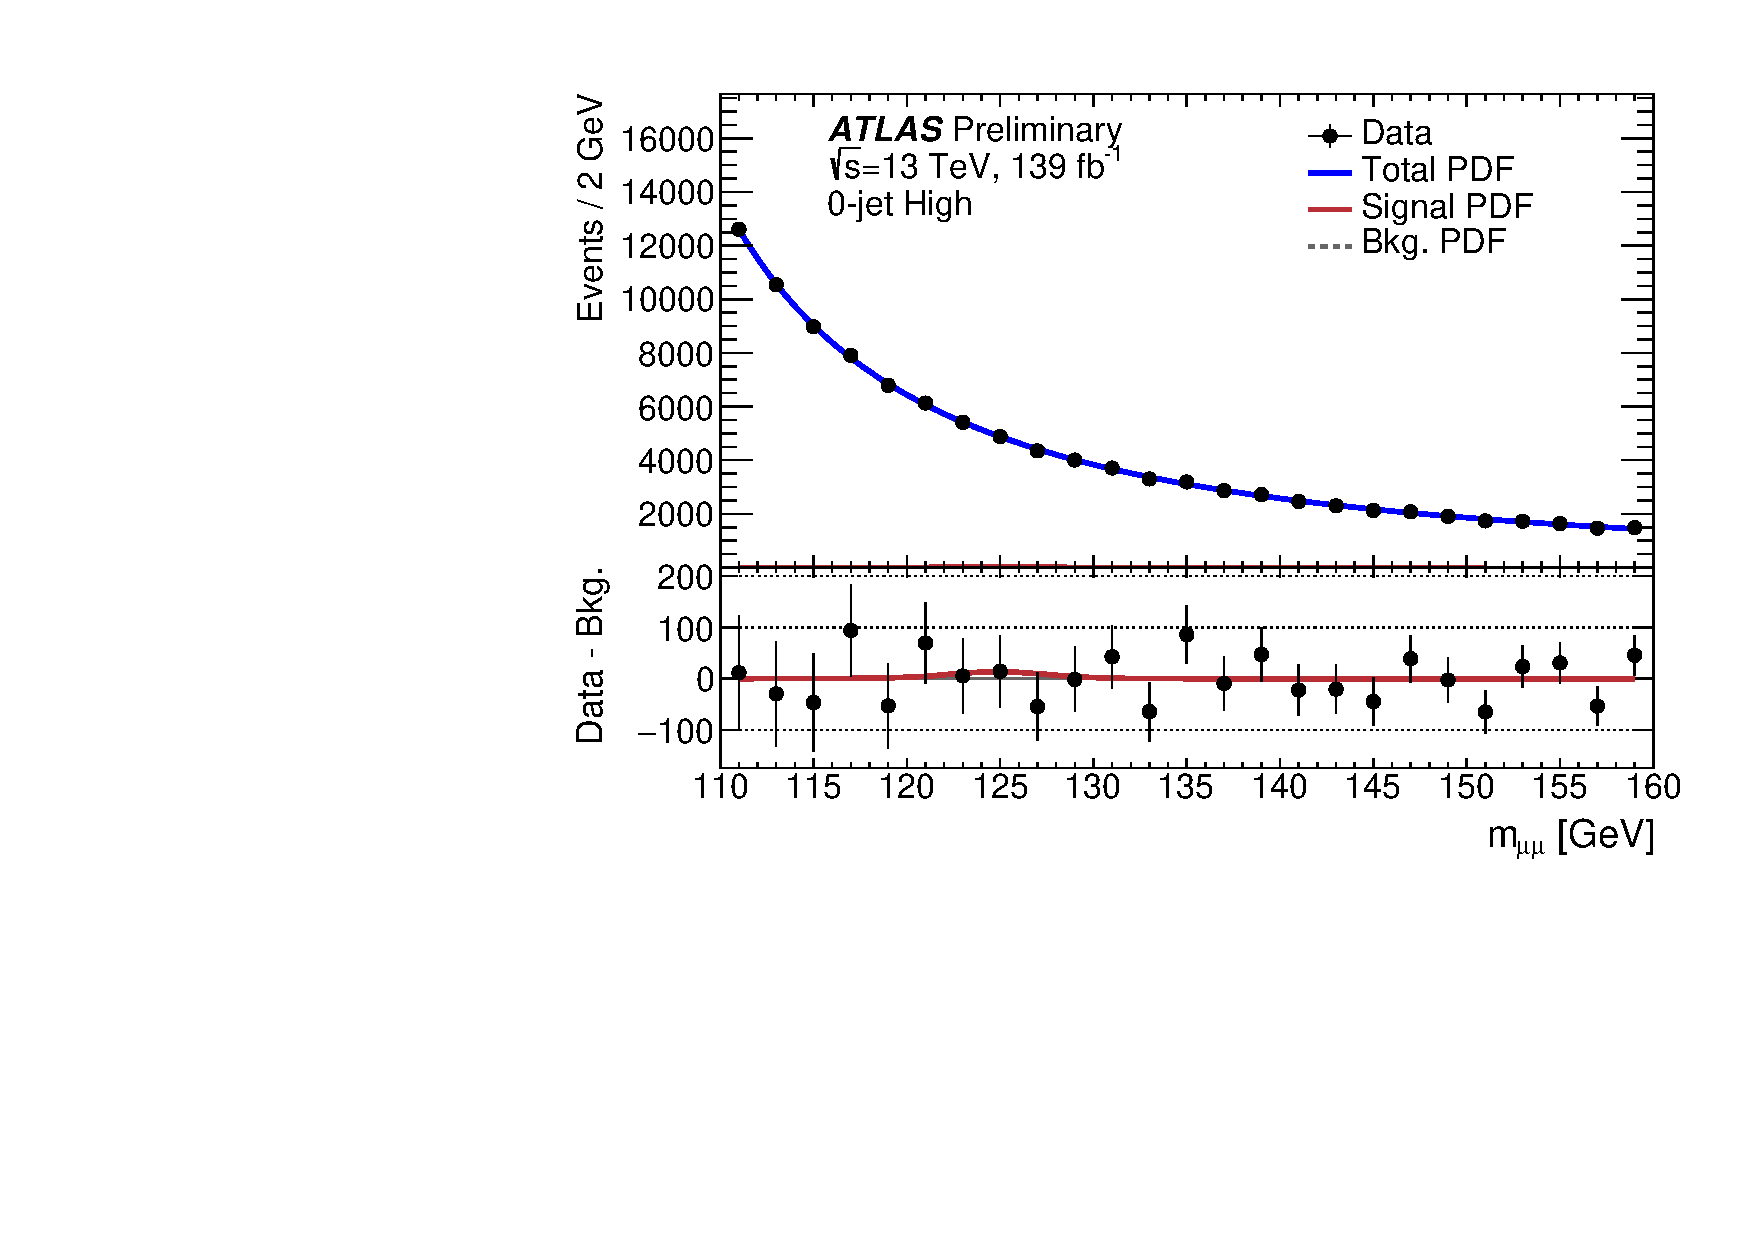
\includegraphics[width=0.49\textwidth]{figures/hmumu/fits/BDT10}
  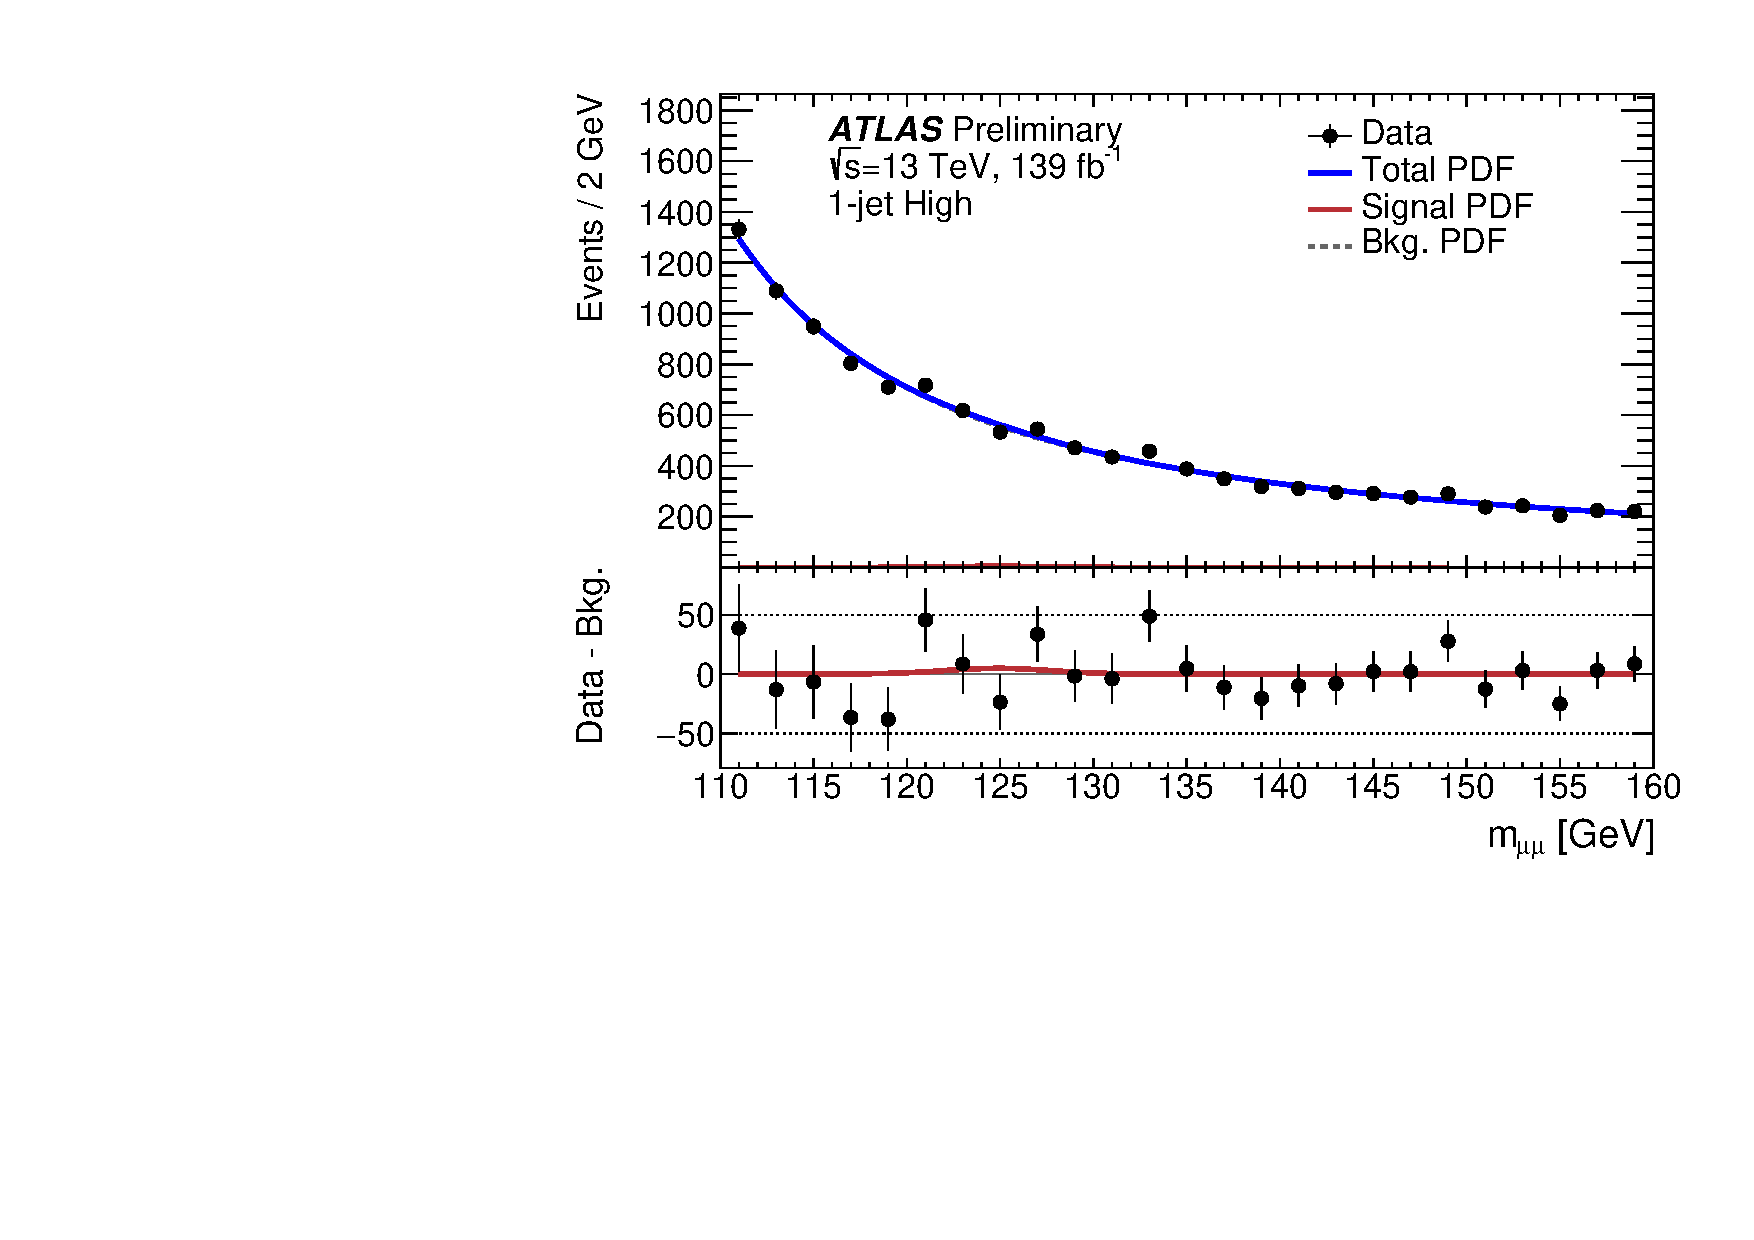
\includegraphics[width=0.49\textwidth]{figures/hmumu/fits/BDT7}
  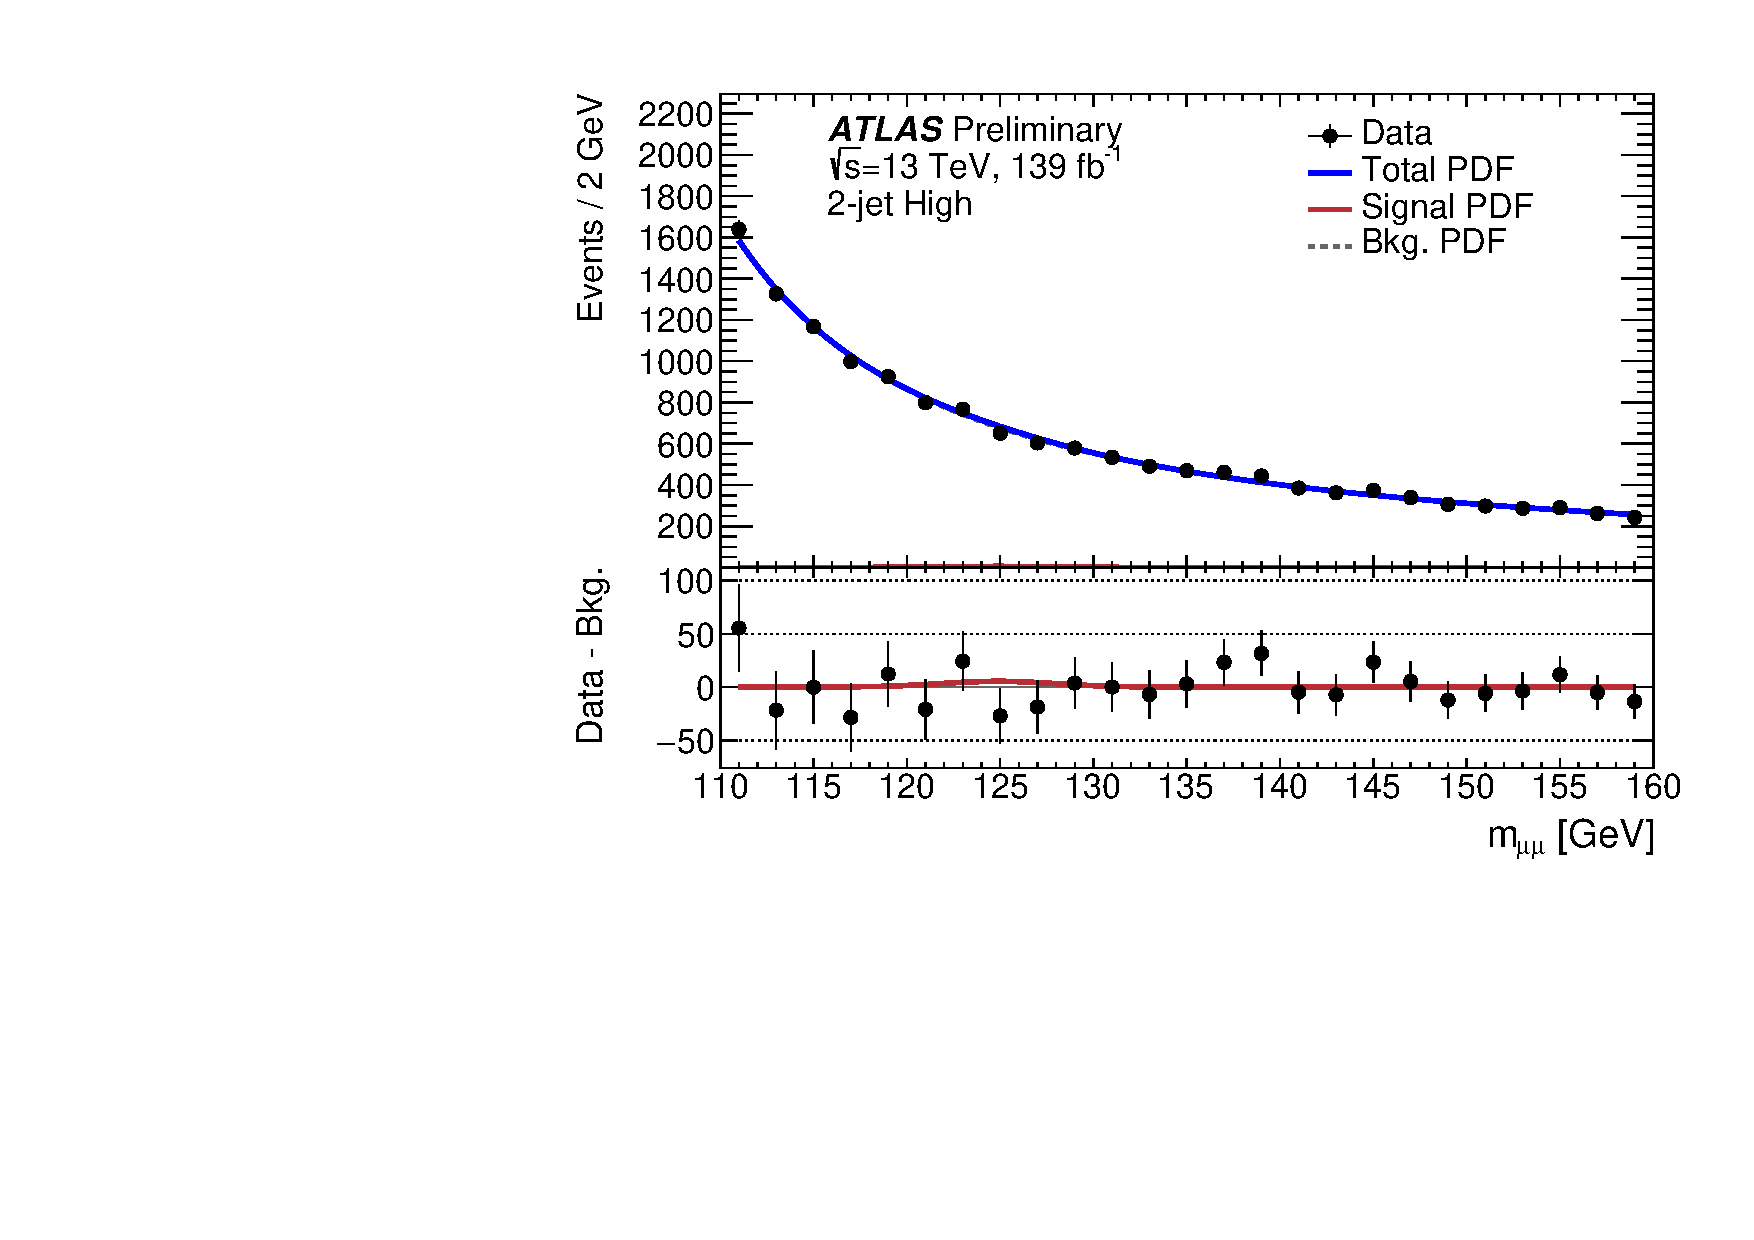
\includegraphics[width=0.49\textwidth]{figures/hmumu/fits/BDT4}
  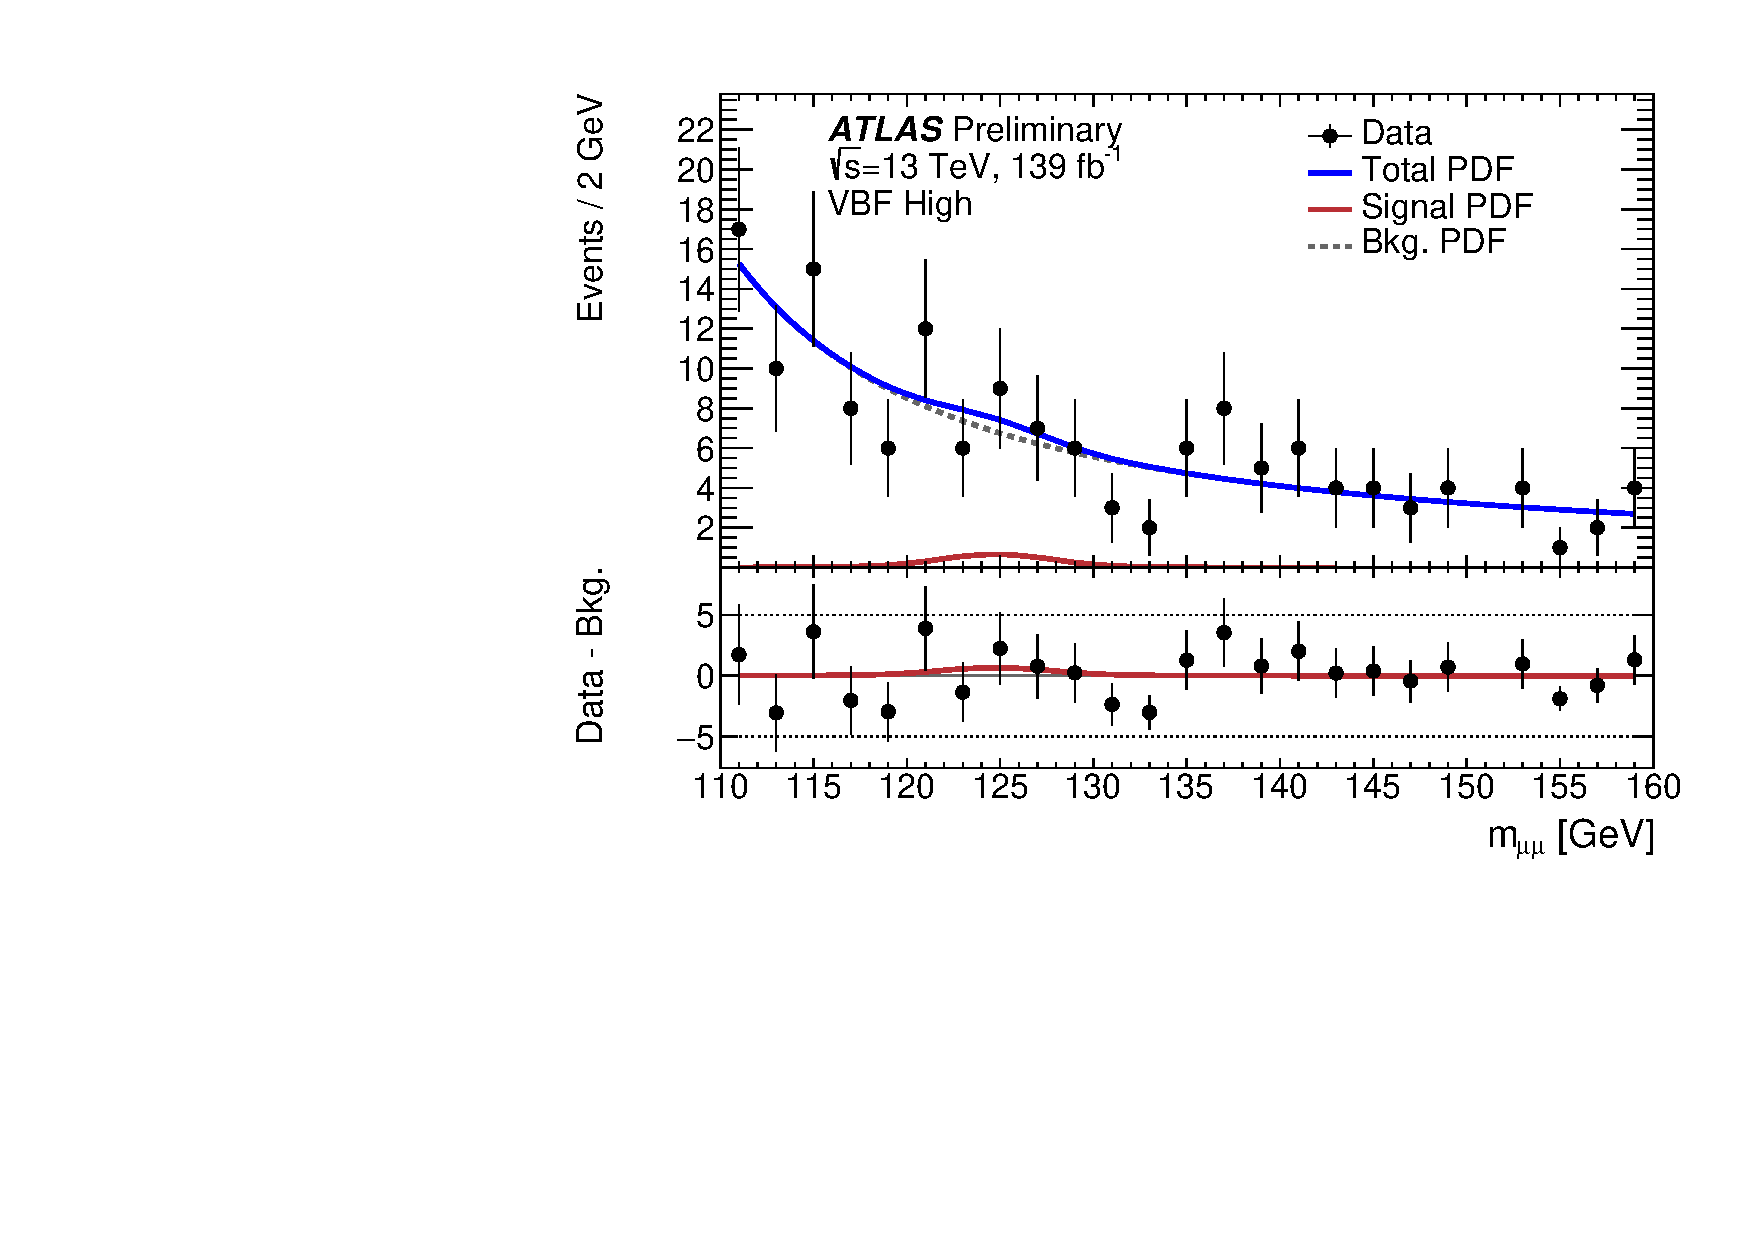
\includegraphics[width=0.49\textwidth]{figures/hmumu/fits/BDT1}
  \caption[Combined signal and background fit to data for High categories]{
  From Ref. \cite{ATLAS-CONF-2019-028}.
  }
  \label{fig:hmumu:fit-high}
\end{figure}


\begin{figure}[h!]
  \centering
  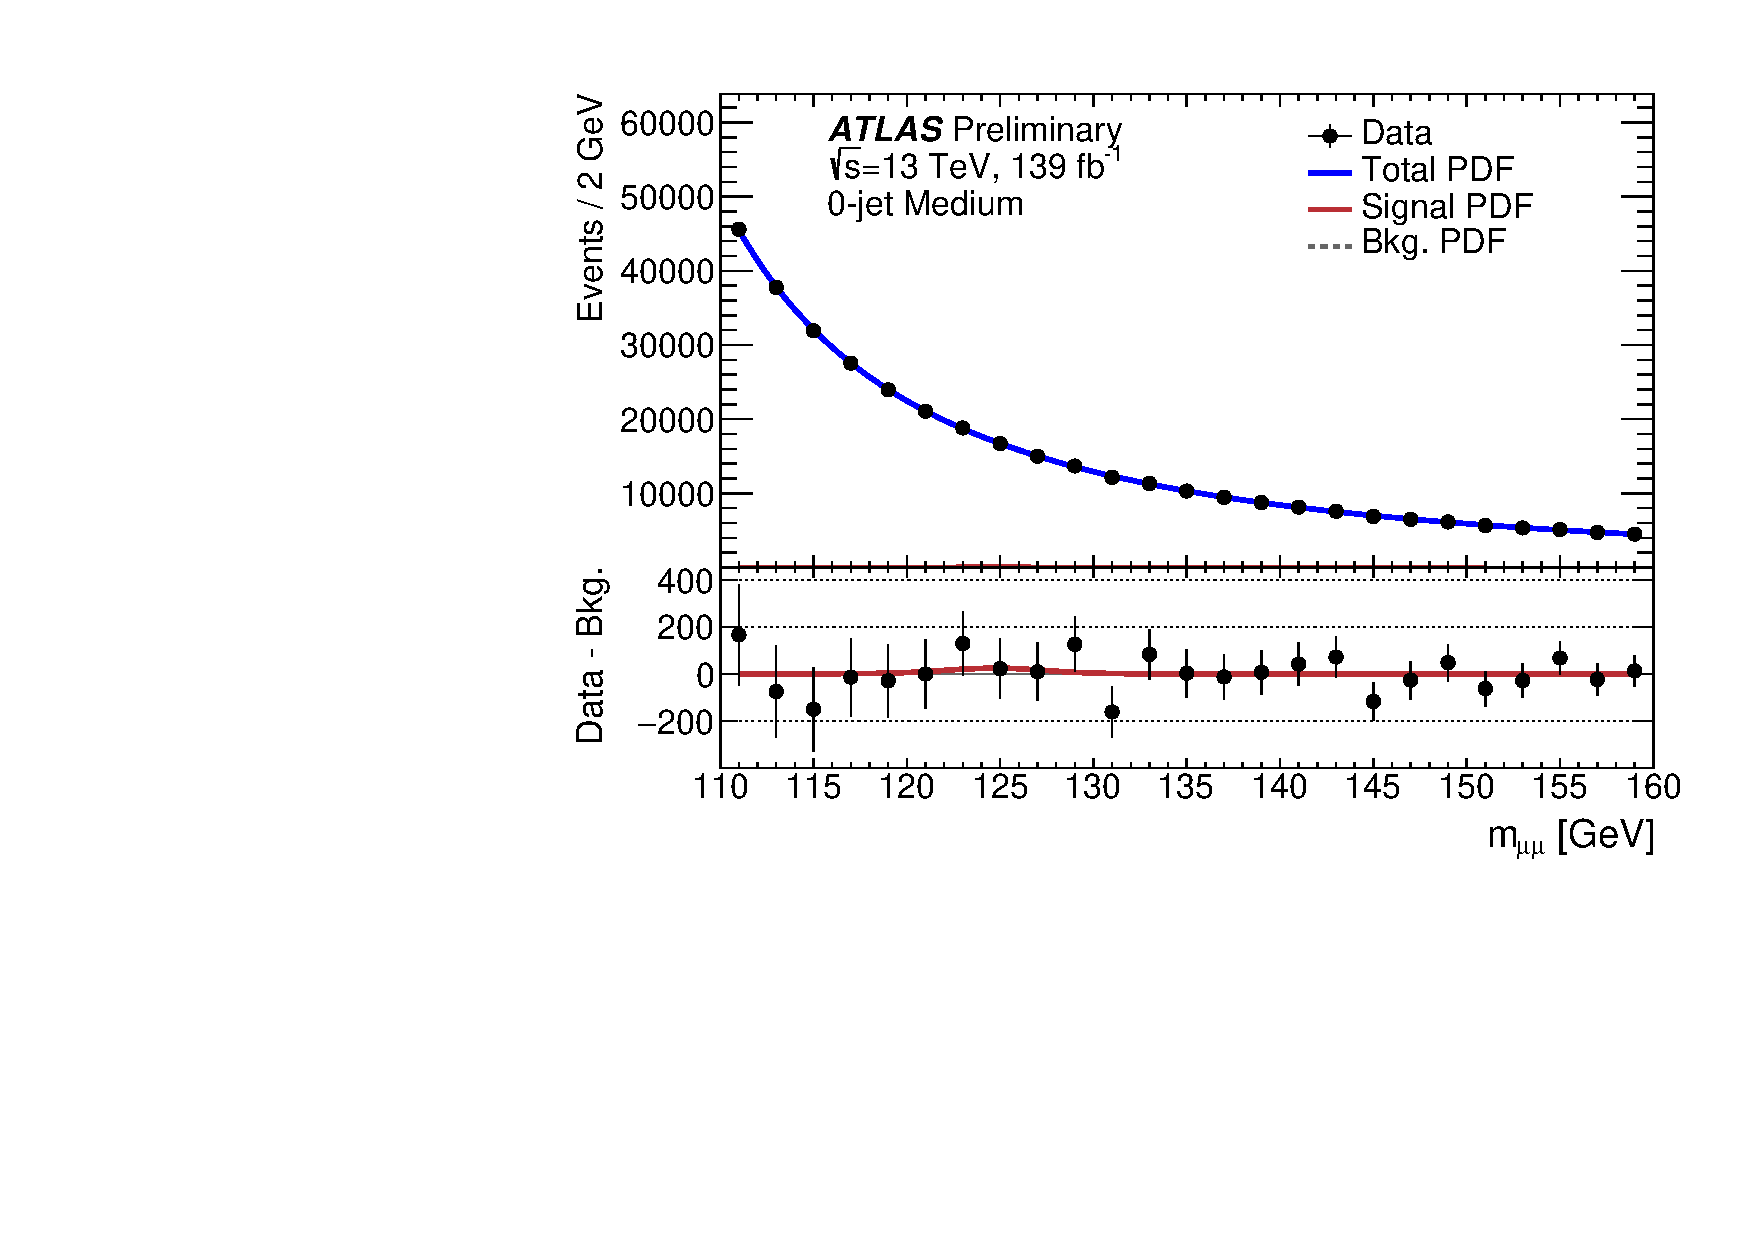
\includegraphics[width=0.49\textwidth]{figures/hmumu/fits/BDT11}
  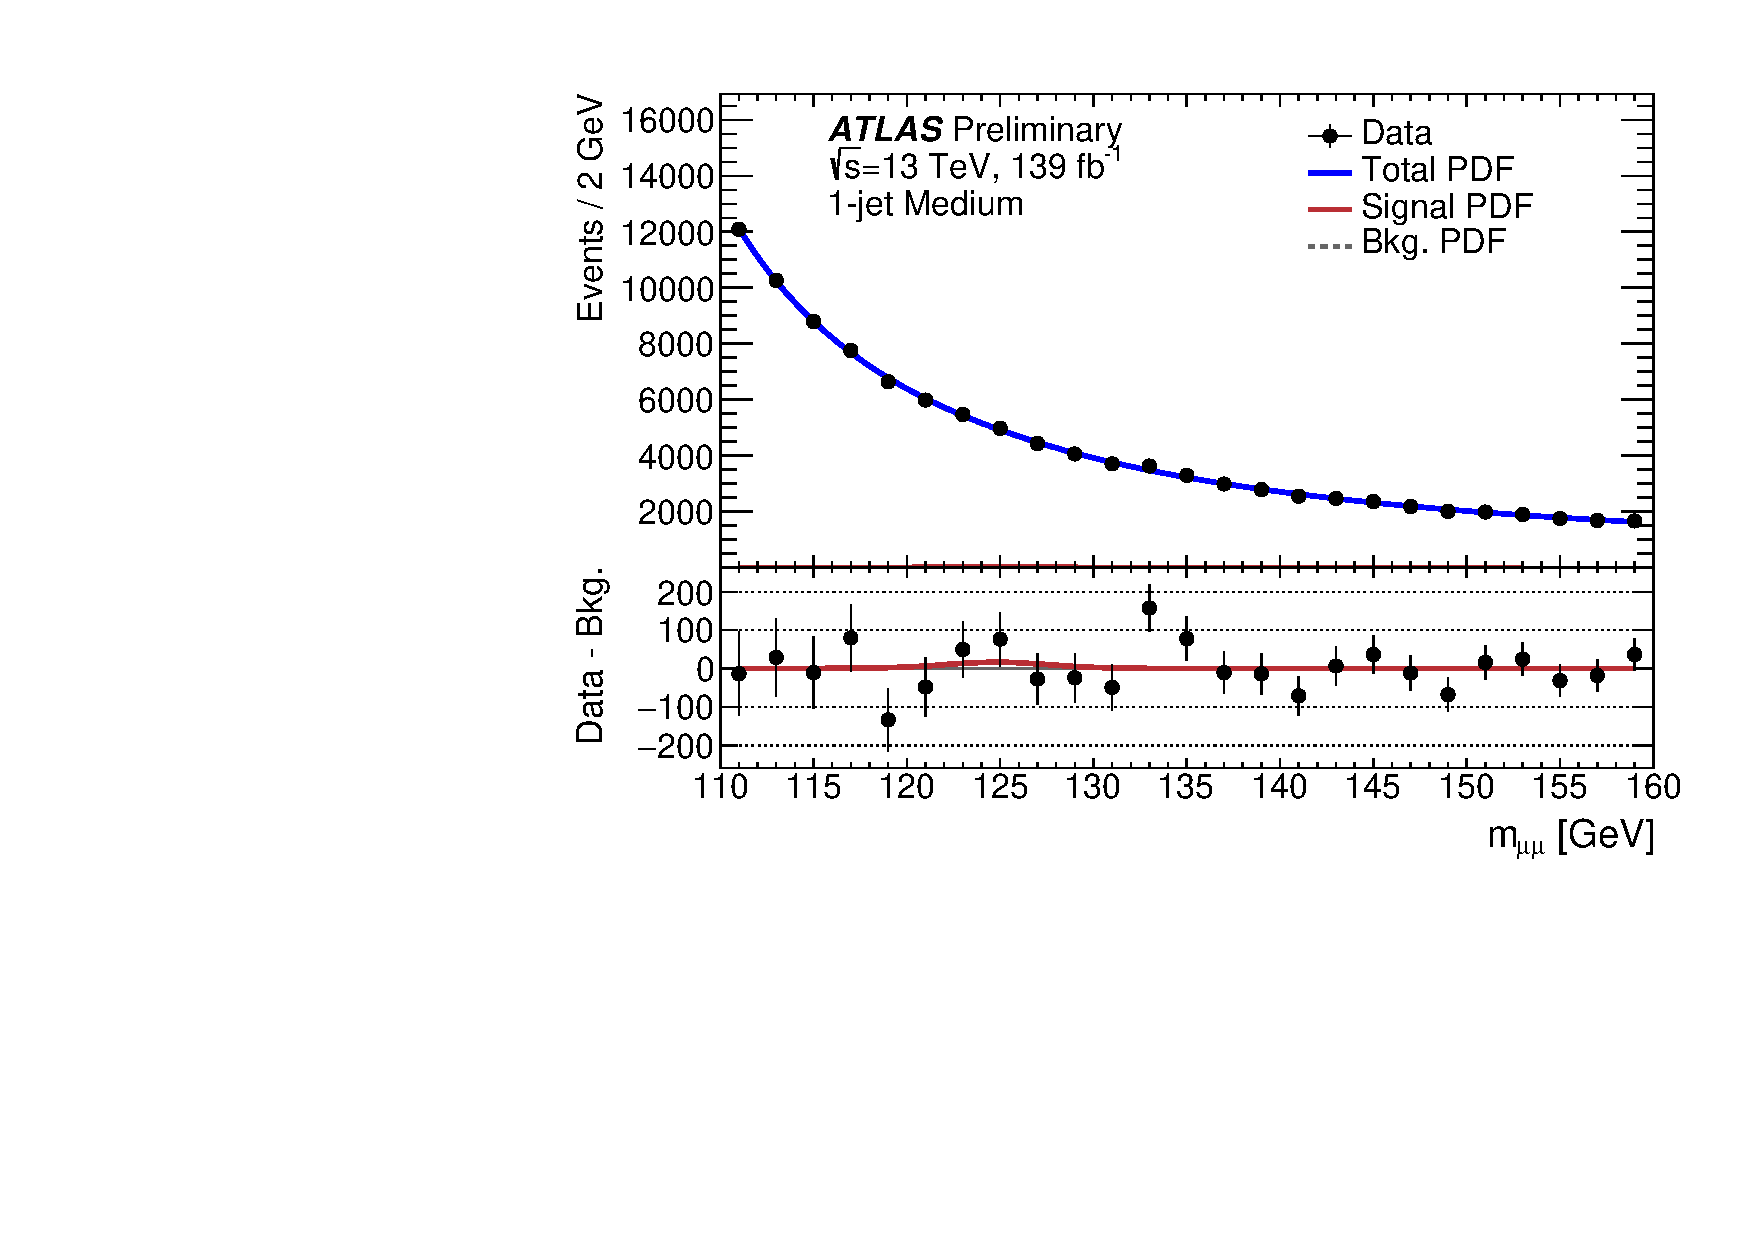
\includegraphics[width=0.49\textwidth]{figures/hmumu/fits/BDT8}
  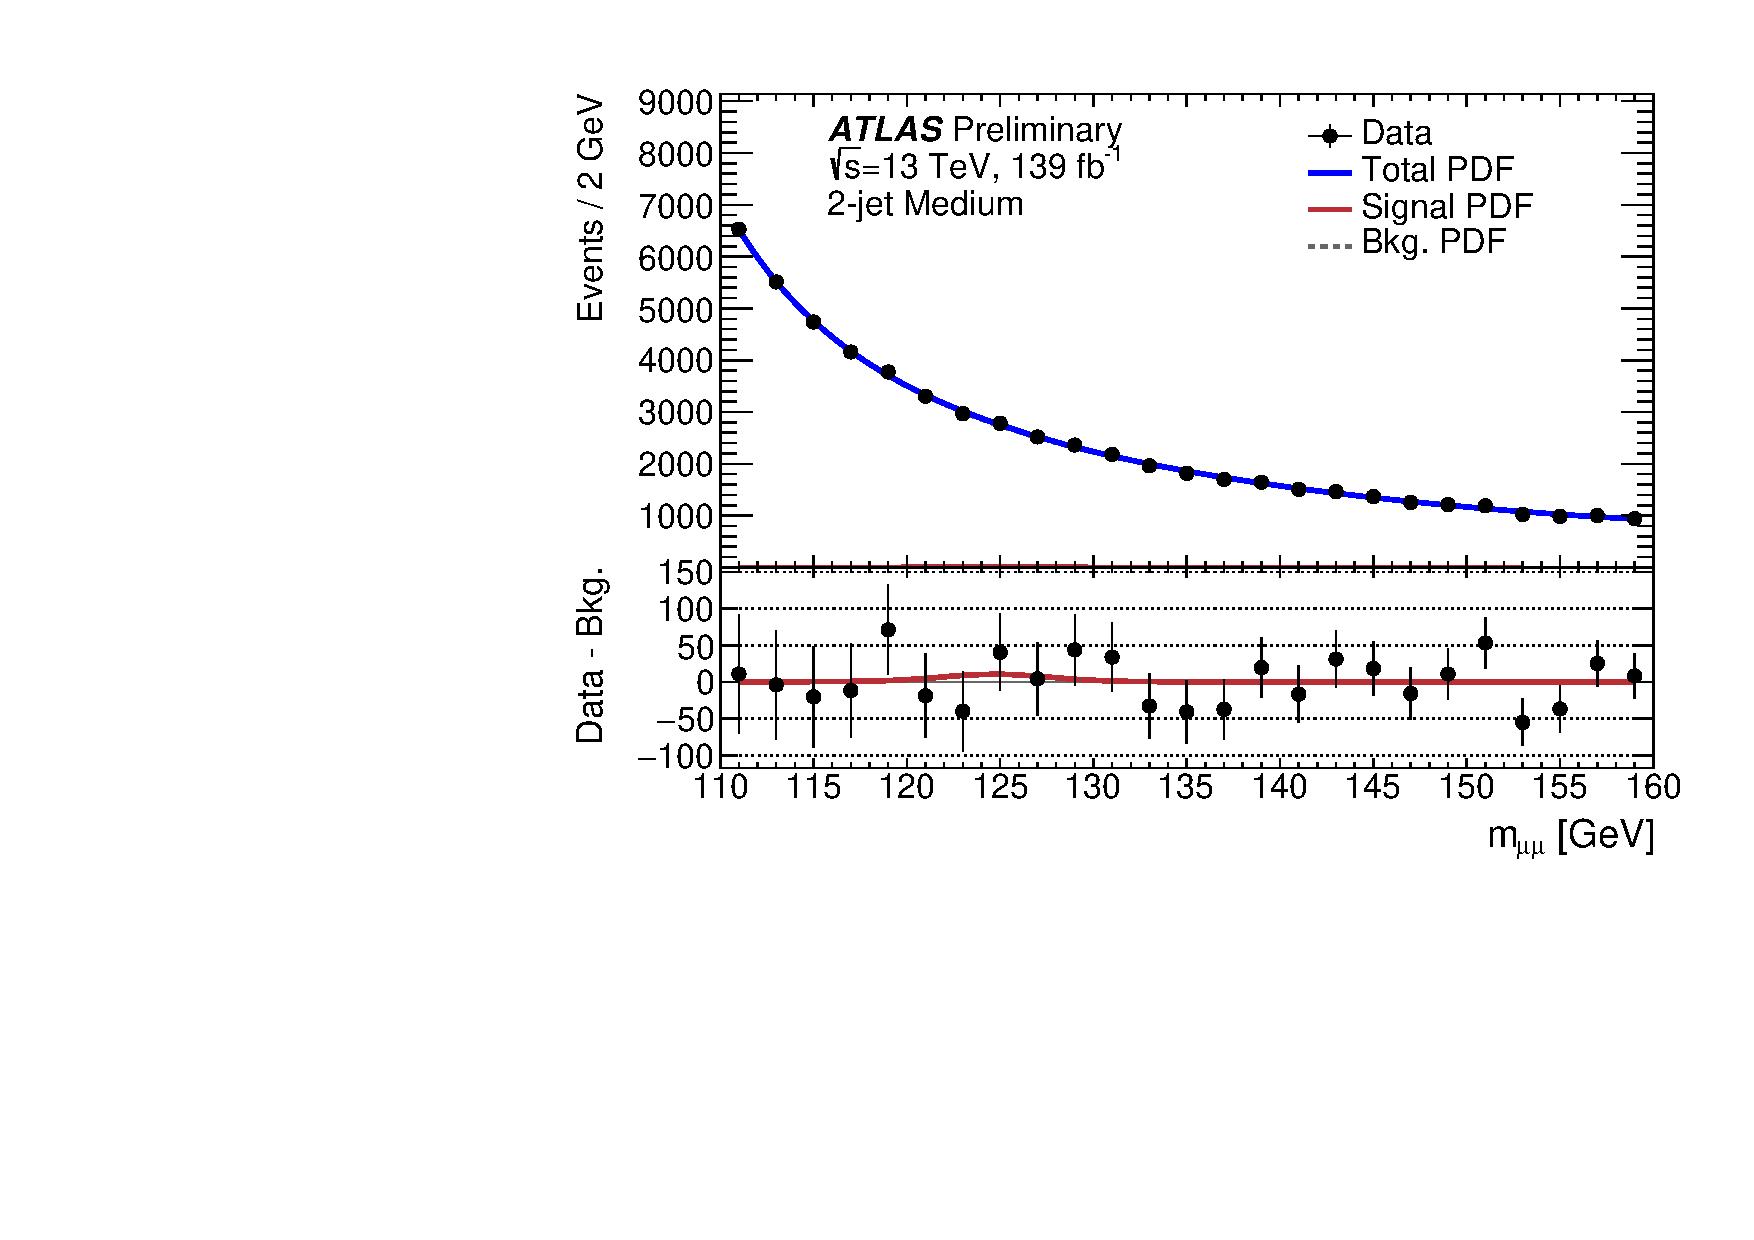
\includegraphics[width=0.49\textwidth]{figures/hmumu/fits/BDT5}
  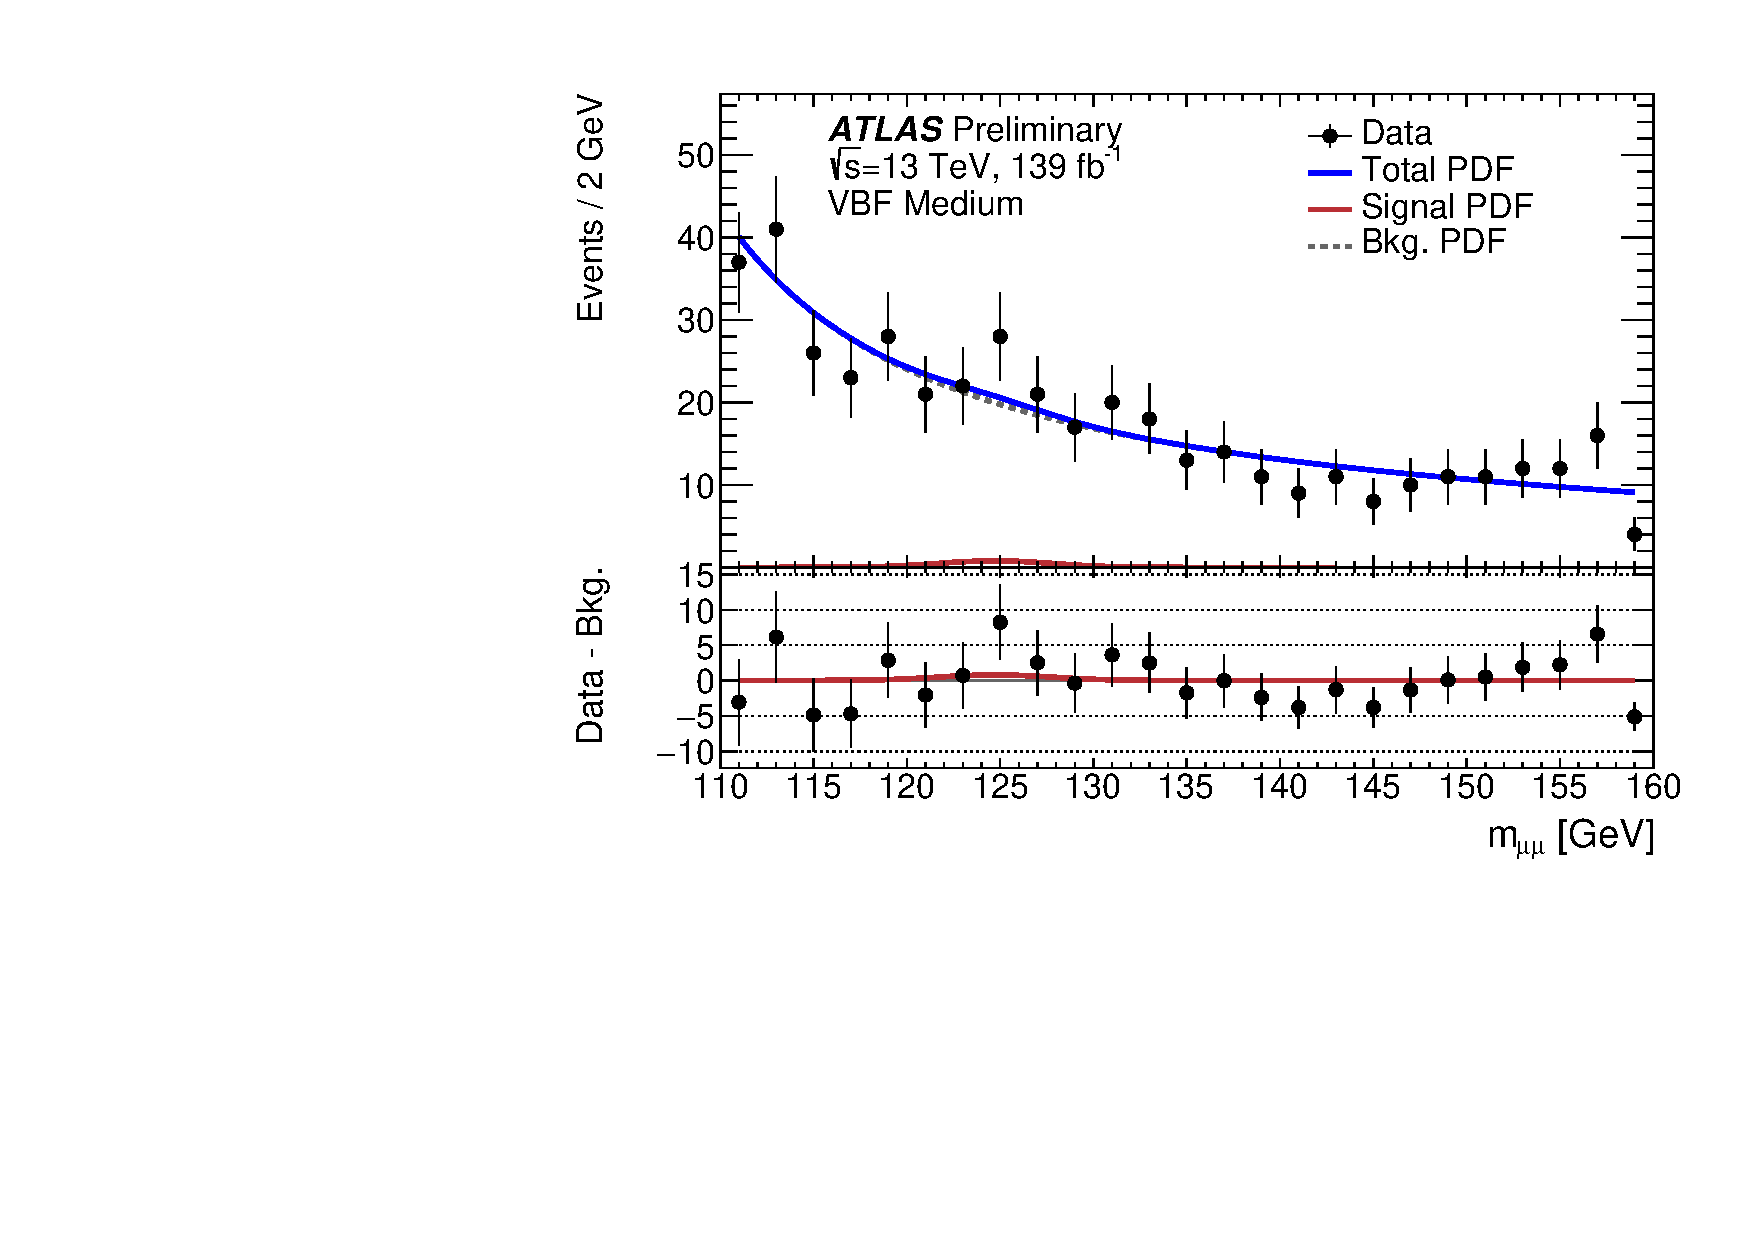
\includegraphics[width=0.49\textwidth]{figures/hmumu/fits/BDT2}
  \caption[Combined signal and background fit to data for Medium categories]{
  From Ref. \cite{ATLAS-CONF-2019-028}.
  }
  \label{fig:hmumu:fit-medium}
\end{figure}



\begin{figure}[h!]
  \centering
  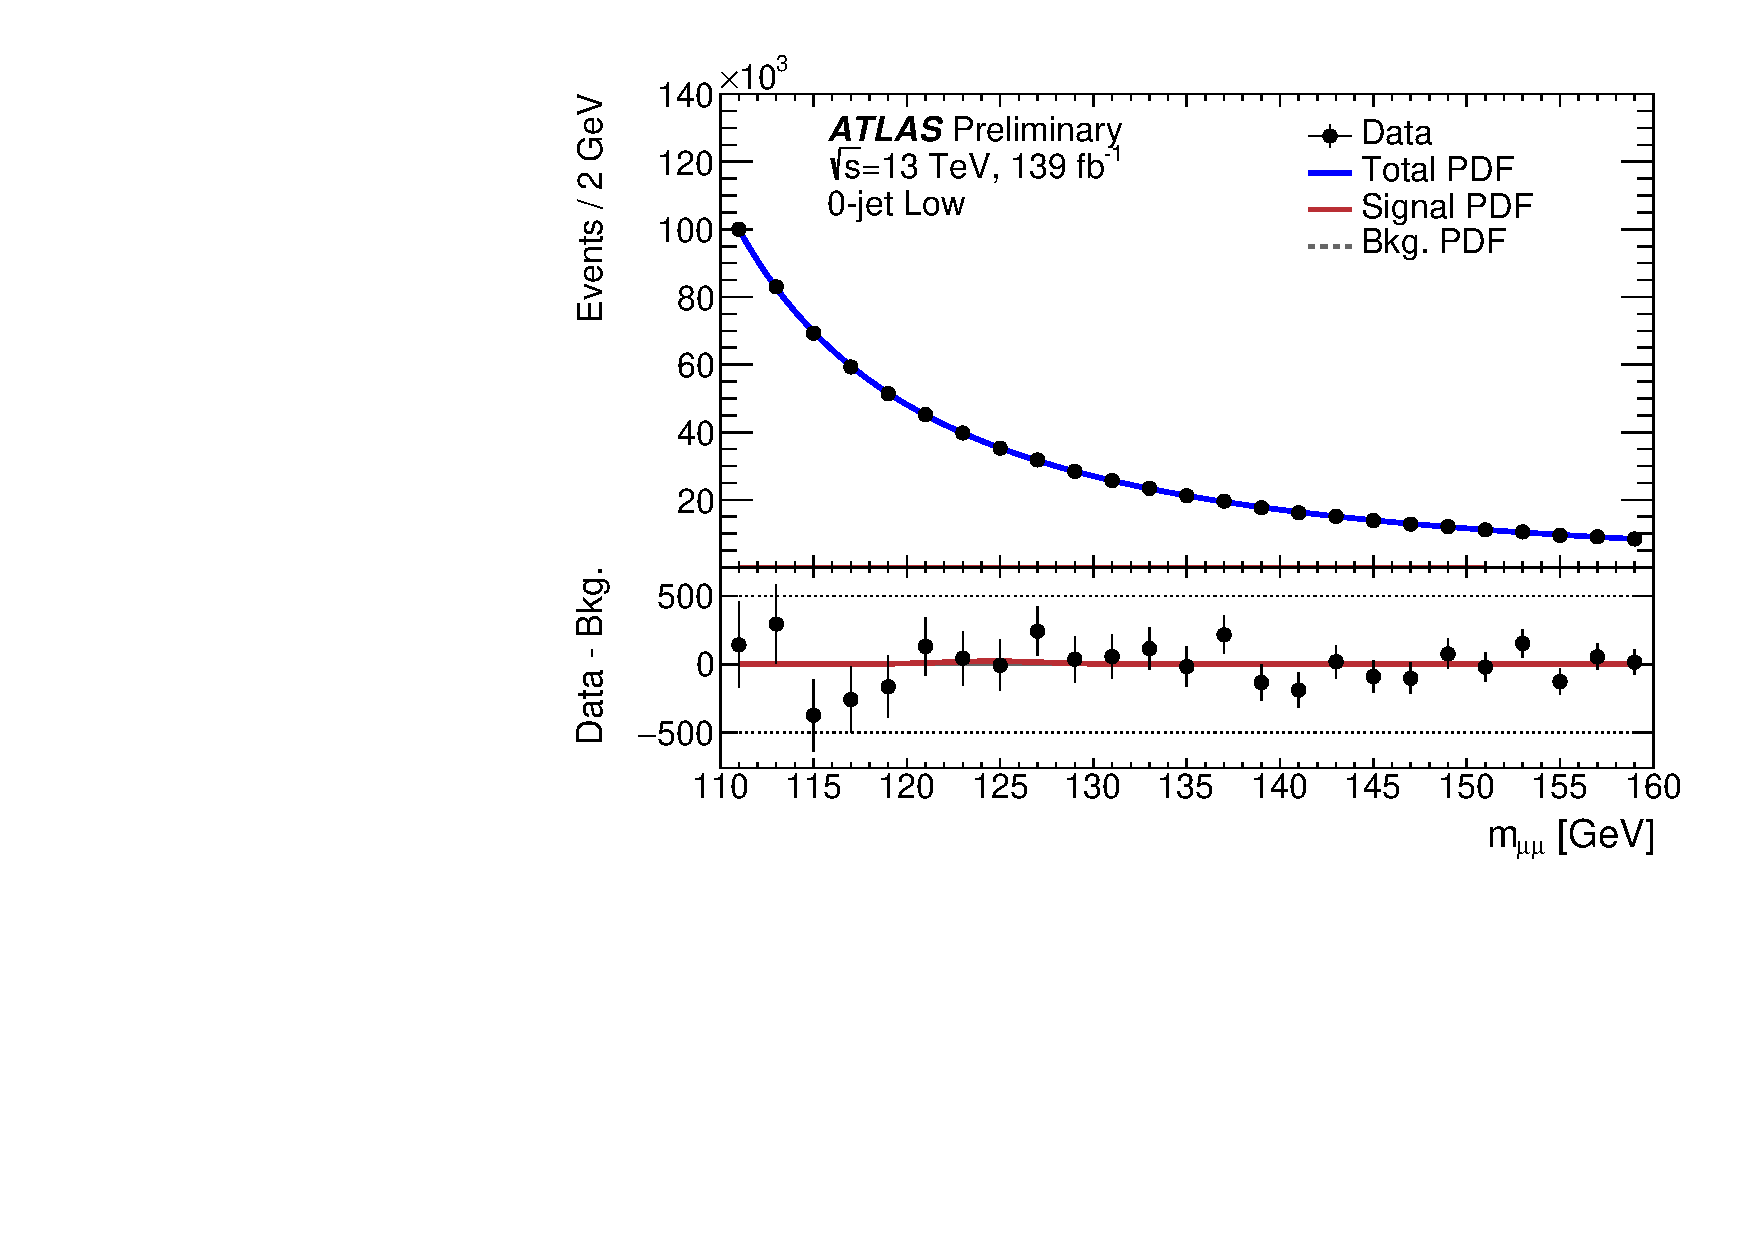
\includegraphics[width=0.49\textwidth]{figures/hmumu/fits/BDT12}
  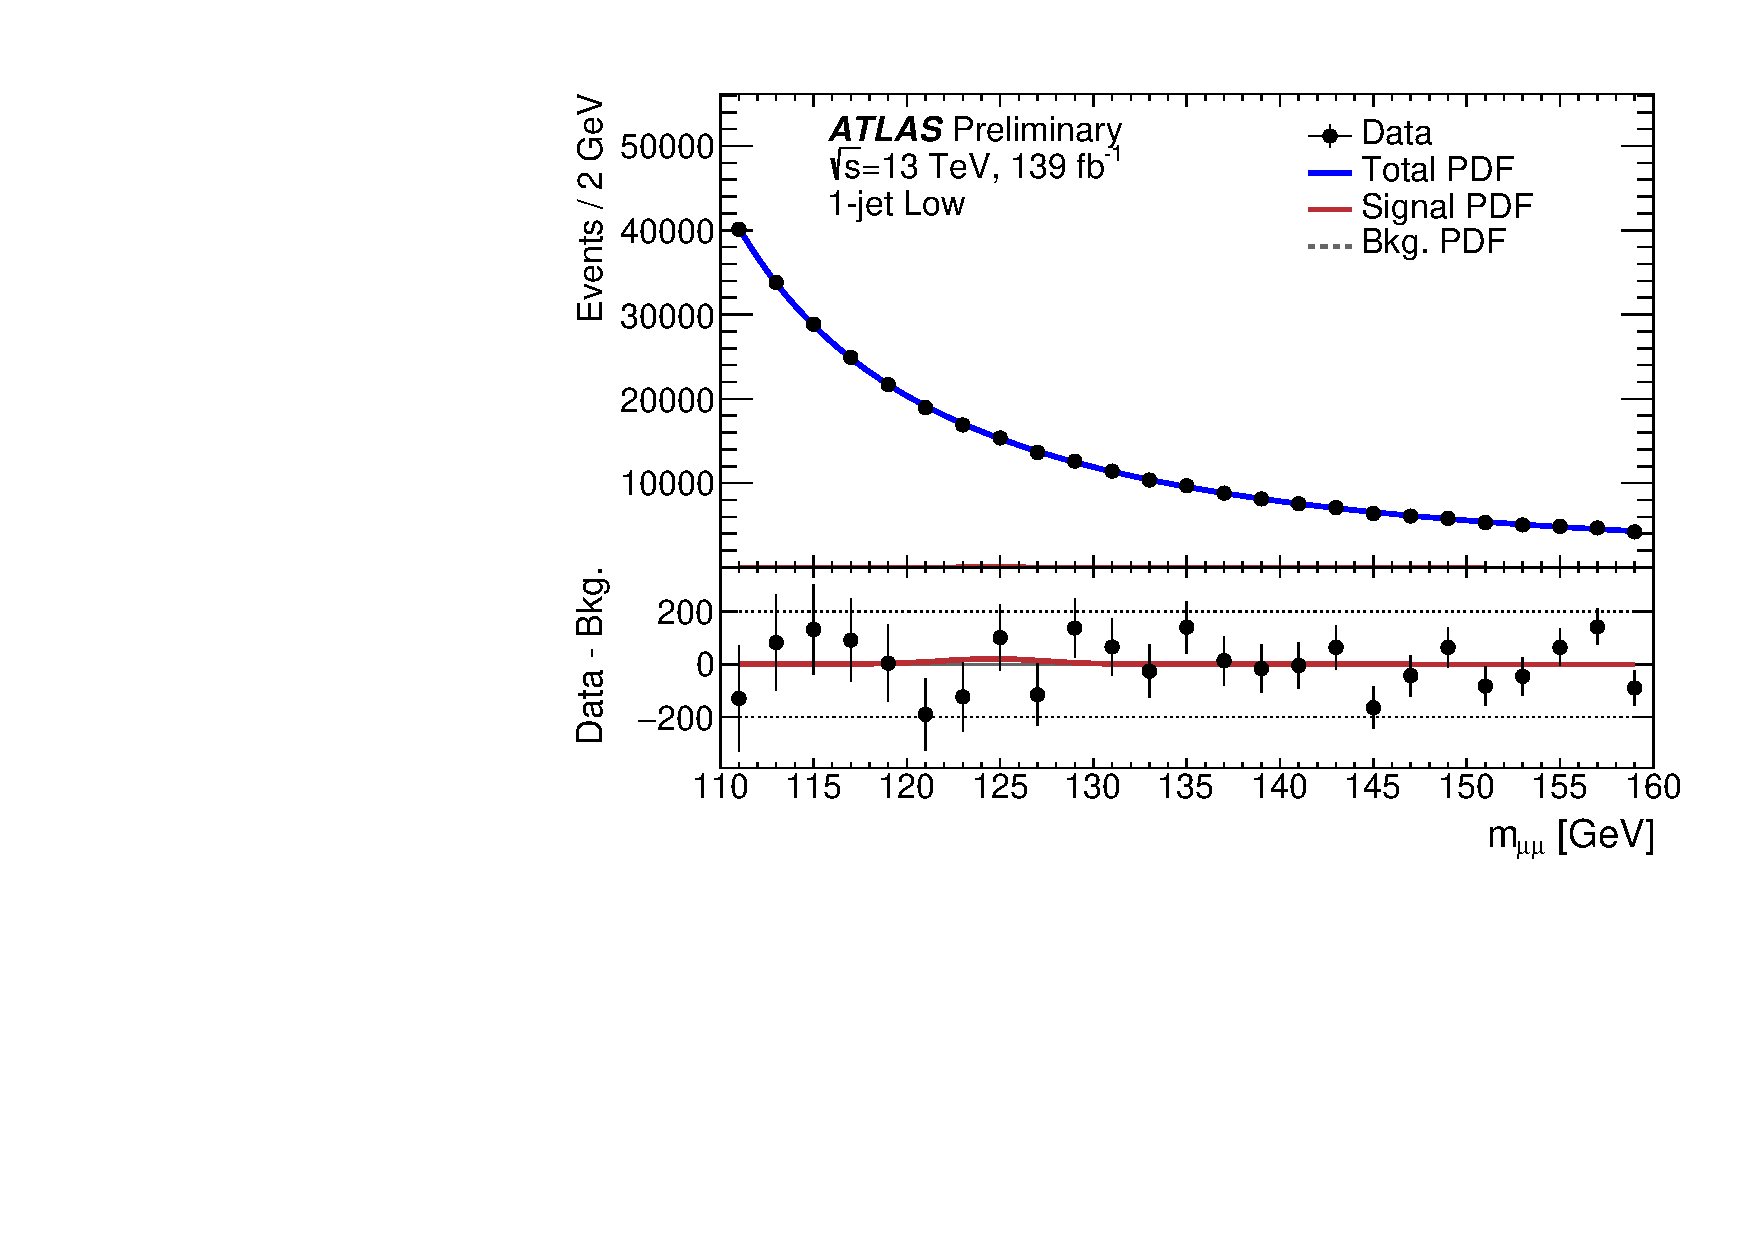
\includegraphics[width=0.49\textwidth]{figures/hmumu/fits/BDT9}
  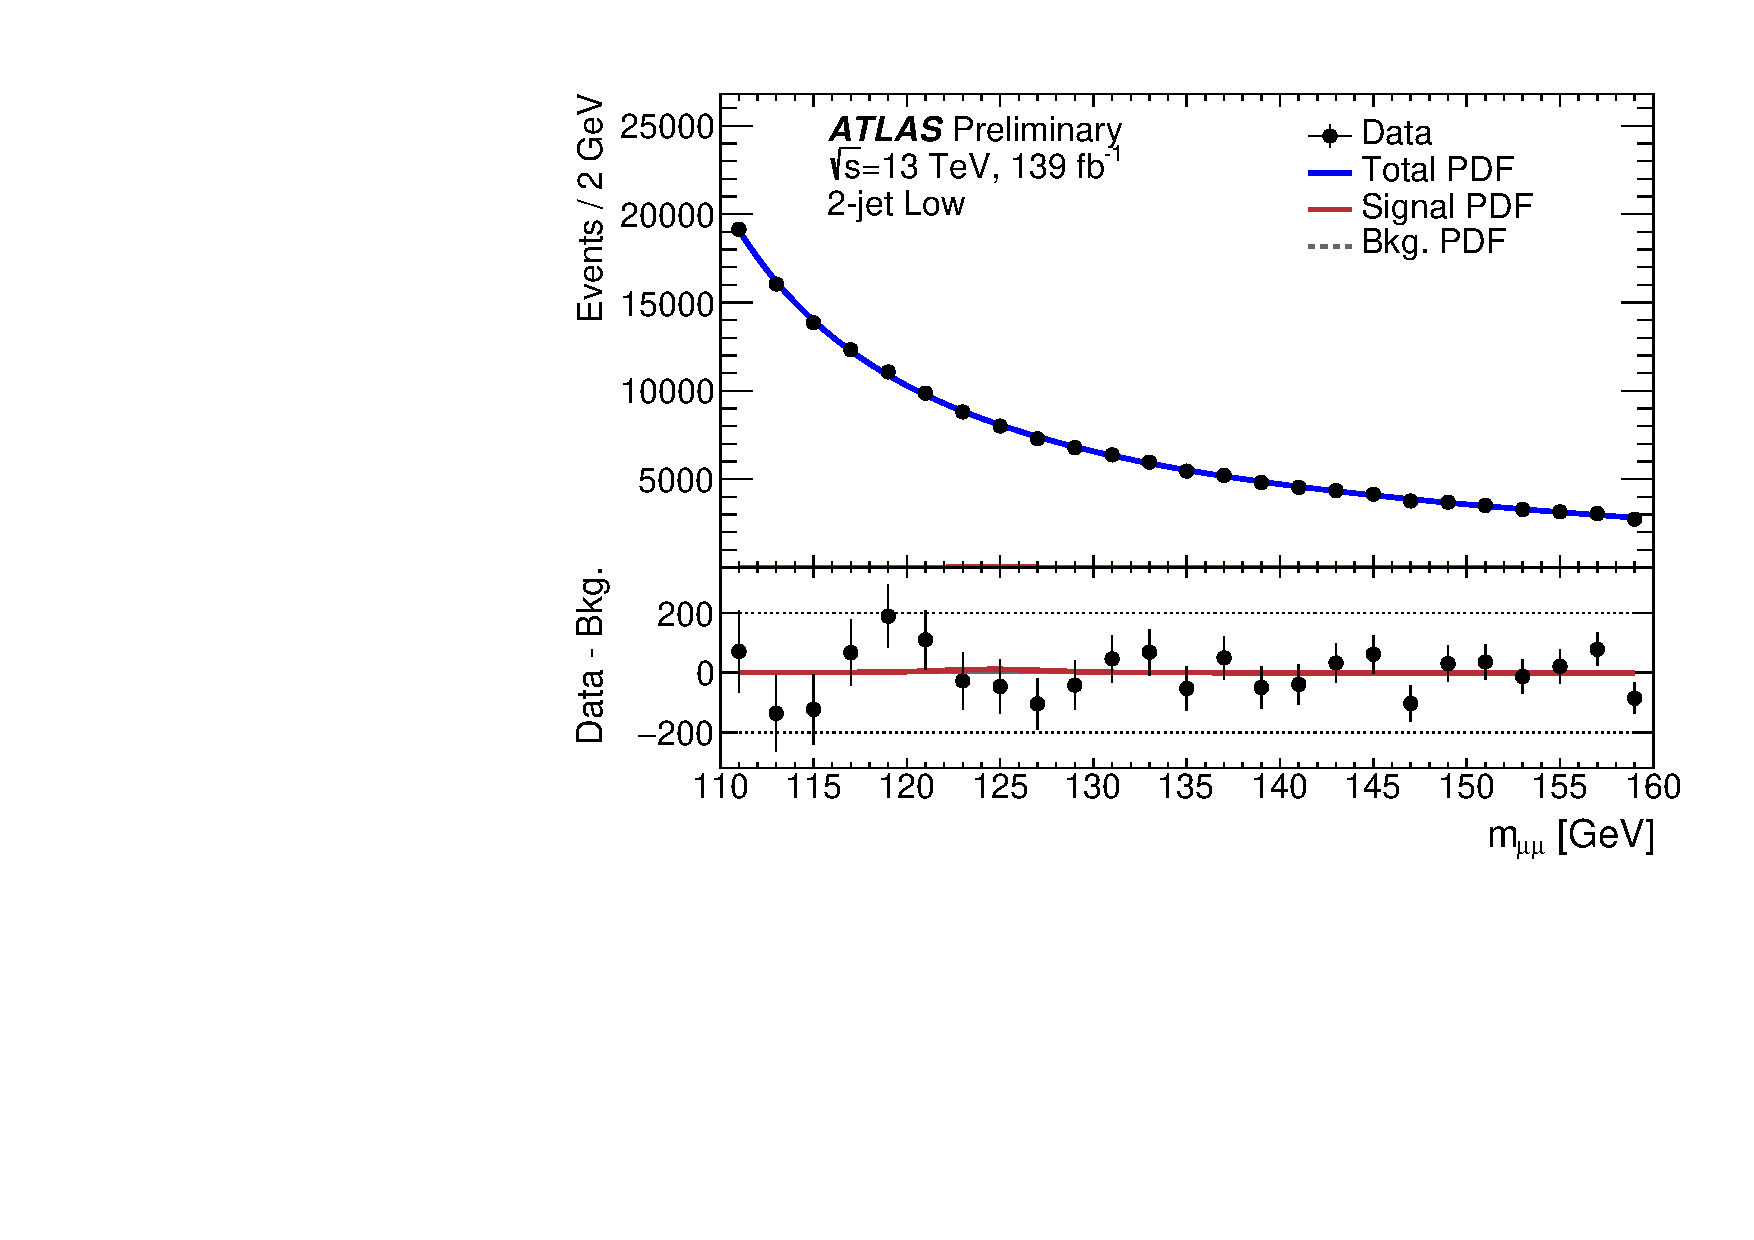
\includegraphics[width=0.49\textwidth]{figures/hmumu/fits/BDT6}
  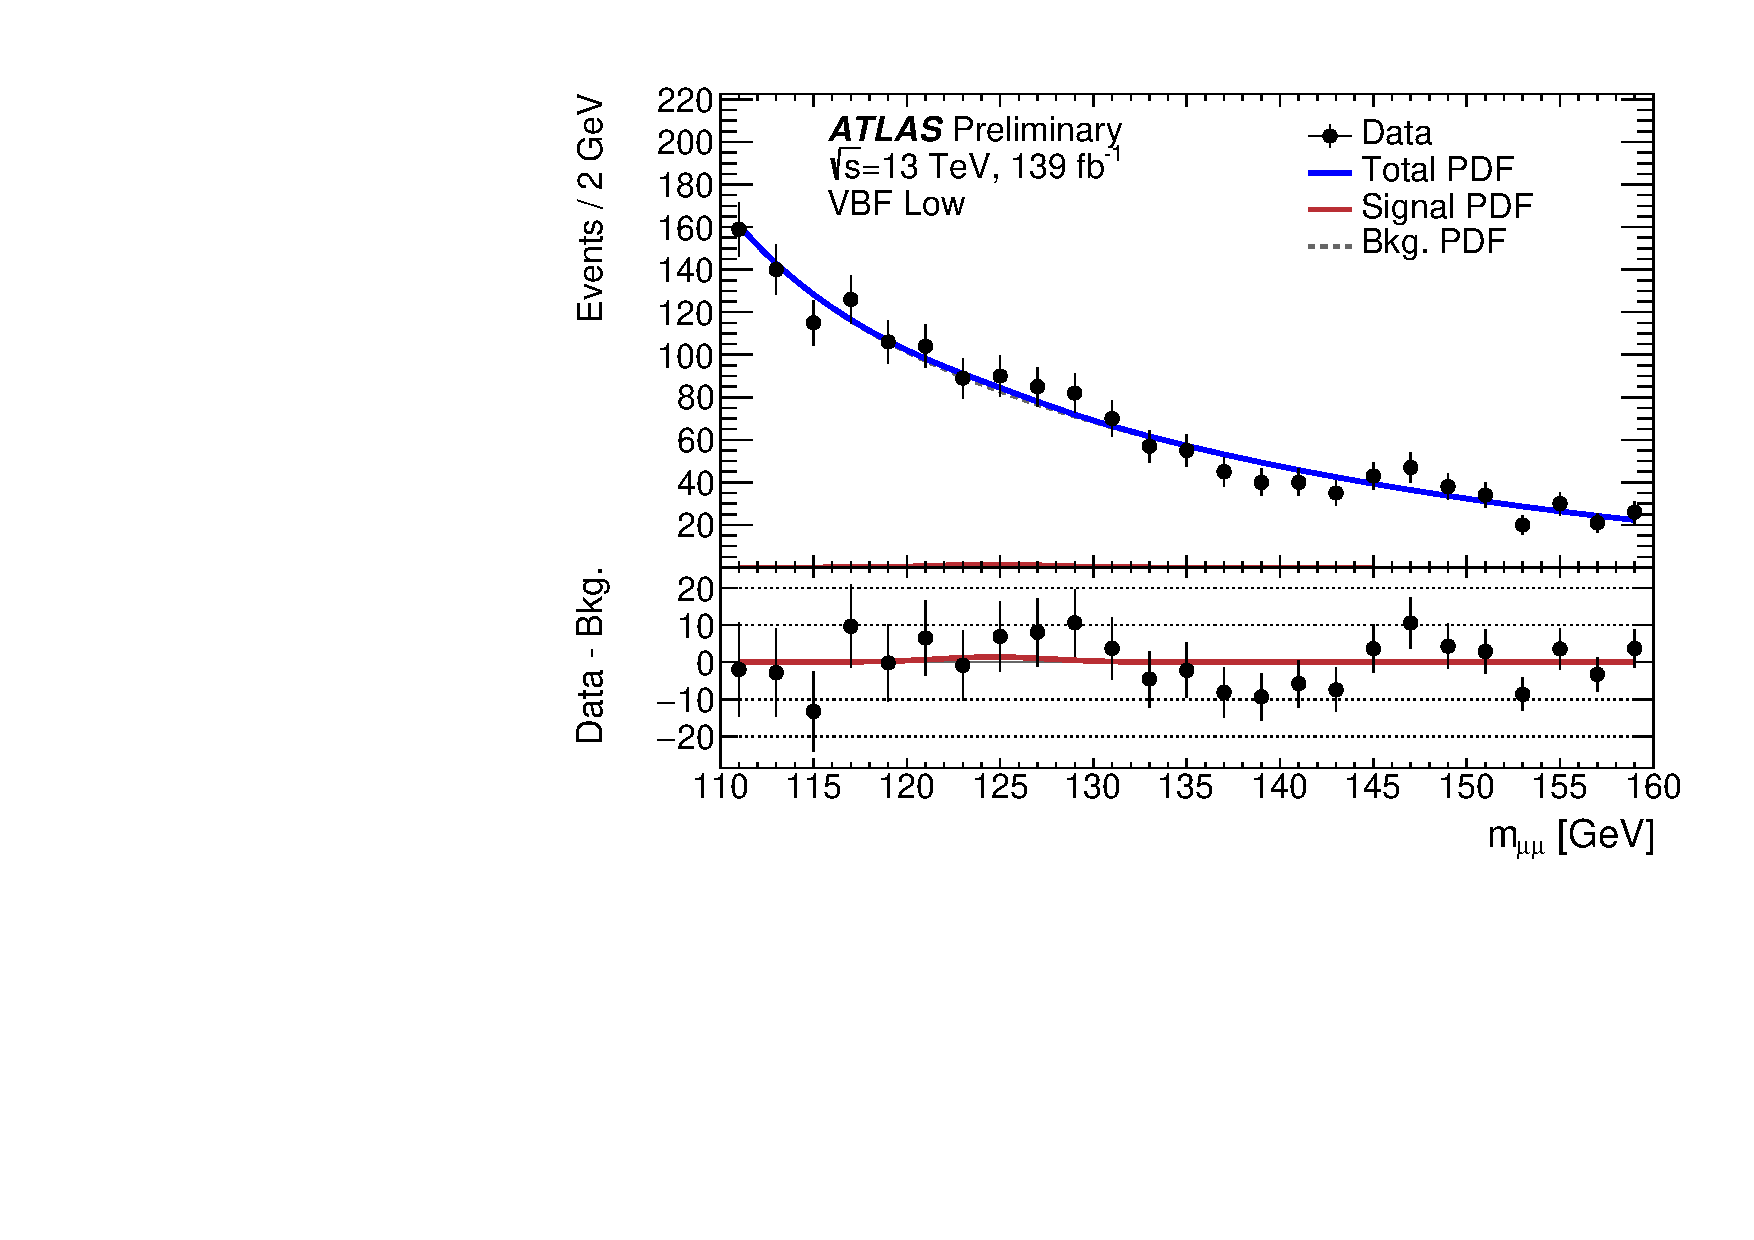
\includegraphics[width=0.49\textwidth]{figures/hmumu/fits/BDT3}
  \caption[Combined signal and background fit to data for Low categories]{
  From Ref. \cite{ATLAS-CONF-2019-028}.
  }
  \label{fig:hmumu:fit-low}
\end{figure}


\begin{figure}[h!]
  \centering
  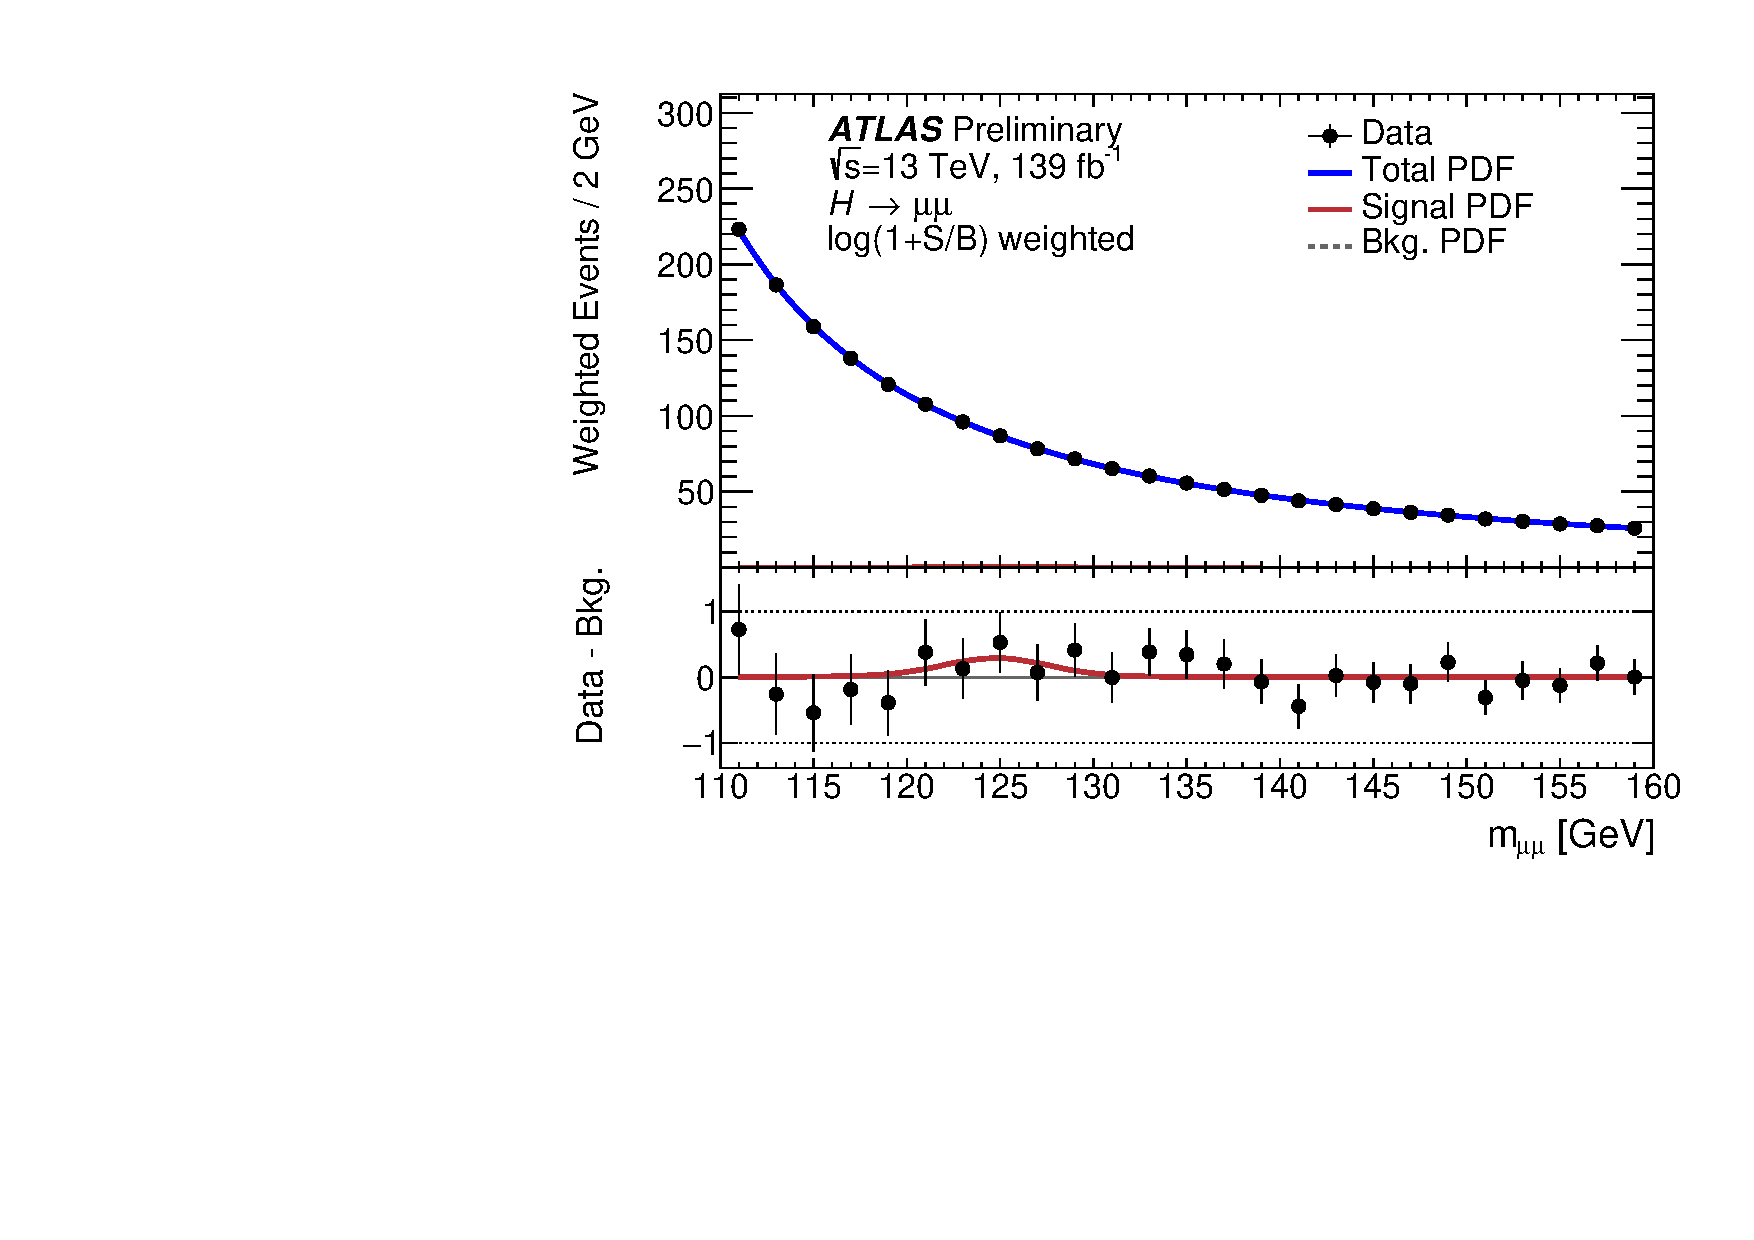
\includegraphics[width=0.7\textwidth]{figures/hmumu/fits/inclusive_w}
  \includegraphics[width=0.7\textwidth]{figures/hmumu/fits/inclusive}
  \caption[Combined signal and background fit to data]{
  From Ref. \cite{ATLAS-CONF-2019-028}.
  }
  \label{fig:hmumu:fit-combination}
\end{figure}







\chapter{Outlook}

\textit{"Prediction is very difficult, especially about the future."}

\vspace{5mm}
\begin{flushright}
--- Niels Bohr
\end{flushright}

\thispagestyle{empty}

\newpage

Sensitivity projections are an essential piece of information for
making informed decisions about the potential future projects the community
should undertake.
It is therefore important to assess what can be achieved with the LHC
machine, and in particular what the physics reach of the full dataset
will be. The dataset is expected to be recorded at 14 \TeV~and to
correspond to 3000 $\ifb$ of integrated luminosity, and is known
as the High-Luminosity LHC programme (HL-LHC).

As a part of the community-wide projections project \cite{ATL-PHYS-PUB-2018-054, Cepeda:2019klc}
an extrapolation of results described in Ref. \cite{ATLAS-CONF-2018-026}
was made. At the time, this was the state-of-the-art analysis.
The general approach of the analysis used in the extrapolation
is not too different from the one described in this thesis. However, a number
of important improvements presented in this thesis, most notably in categorisation
and background modelling, that result in approximately 25\% improvement
in sensitivity of the analysis, are not taken into account in the projection.

In addition to the increase in integrated luminosity from 80 to 3000 $\ifb$,
increases in the production cross-sections from 13 to 14 \TeV~are also
taken into account. The signal yields are scaled according to the
values in Ref. \cite{deFlorian:2016spz}, separately for the $\ggf$
and VBF production modes. The background yields are scaled according
to the parton luminosity ratio as described in Ref. \cite{Heinemeyer:2013tqa},
taking into account that the backgrounds are produced predominantly via
the interaction of quarks.

The performance of the reconstruction of physics objects is assumed
to remain unchanged to simplify the extrapolation. While the higher
\pileup~is likely to degrade performance this is expected to be
roughly balanced by the improved performance of the ATLAS detector.
Muon resolution is an exception to this rule because of the
large expected improvements in performance of the ATLAS Inner Tracker (ITk)
upgrade. To model this improvement the signal widths are reduced 
by 30\% in the VBF and Central analysis categories and by 15\% in
the Forward categories to emulate the expected improvements
\cite{Collaboration:2285585}.

Two scenarios are considered regarding the treatment of systematic
uncertainties. Scenario 1 (S1) assumes the relative systematic
uncertainties remain as they are today, while in Scenario 2 (S2)
most of the theoretical uncertainties on the signal normalisation
are halved, with the exception of the PDF uncertainties for which the reduction factors depend on the quark/gluon
initial states \cite{Khalek:2018mdn}. The
spurious signal uncertainty is assumed to be negligible in both the S1
and S2, while the luminosity uncertainty is set to 1\%.

Table \ref{tab:out:res} shows the comparison of the expected uncertainty
on the signal strength for the Run 2 analysis with 79.8 $\ifb$
and the S1 and S2 scenarios at the HL-LHC. It can be seen that 
even with the full HL-LHC dataset the analysis will be limited
by the statistical uncertainty on data. Not taken into account in the results in Table \ref{tab:out:res} is
an additional 25\% improvement in sensitivity that can be expected
from the improved background modelling and categorisation
presented in this thesis.

\begin{table}[htb]
  \renewcommand{\arraystretch}{1.3}
  \centering
  \caption{
    The expected uncertainties on the signal strength measurement with
    the Run 2, 79.8 $\ifb$ dataset and the S1 and S2 systematic
    uncertainty scenarios for the HL-LHC dataset. Columns show
    the total uncertainty, statistical uncertainty, experimental
    systematic uncertainty, and the uncertainty on the signal
    normalisation.
    Reproduced from Ref. \cite{ATL-PHYS-PUB-2018-054}.}
  \label{tab:out:res}
  \begin{tabular}{ccccc}
    \toprule
    \midrule
    Scenario & $\Delta_\text{tot}/\sigma_\text{SM}$ 
             & $\Delta_\text{stat}/\sigma_\text{SM}$ 
             & $\Delta_\text{exp}/\sigma_\text{SM}$ 
             & $\Delta_{\mu_\text{sig}}/\sigma_\text{SM}$ \\
    \midrule
    Run 2, 79.8 $\ifb$ & $^{+1.04}_{-1.06}$ & $^{+0.99}_{-1.03}$ & $^{+0.03}_{-0.03}$ & $^{+0.32}_{-0.27}$ \\
    HL-LHC S1          & $^{+0.15}_{-0.14}$ & $^{+0.12}_{-0.13}$ & $^{+0.03}_{-0.03}$ & $^{+0.08}_{-0.05}$ \\
    HL-LHC S2          & $^{+0.13}_{-0.13}$ & $^{+0.12}_{-0.13}$ & $^{+0.02}_{-0.02}$ & $^{+0.05}_{-0.04}$ \\
    \midrule
    \bottomrule
  \end{tabular}
\end{table}

This is in good agreement with a previous study of $\hmumu$ prospects
\cite{ATL-PHYS-PUB-2018-006} based on generator-level MC simulation.
That study simulated a dataset equivalent to 3000 $\ifb$ collected at 14
\TeV~with the average number of interactions per bunch crossing
$\langle \mu \rangle = 200$, and the most up-to-date detector performance.
The projected accuracy of the signal strength measurement was found to
be 13\%, while the discovery significance was found to be larger than
9 $\sigma$.

Additionally, it is worth presenting a simple extrapolation of the results
presented in this thesis to the near future. The reason is that the
analysis is approaching the significance threshold considered as 
evidence (3 $\sigma$), and that a considerable improvement of $\sim 25\%$
has been made over the iteration of the analysis on which the more detailed
projection was based. Assuming that the discovery significance as well as the
uncertainty on the signal strength scale with luminosity as
$1/\sqrt{\mathcal{L}}$, which is reasonable for the near future,
the 3 $\sigma$ benchmark will be reached with 560 $\ifb$, and the 5 $\sigma$
benchmark with 1550 $\ifb$, while the 0.5 uncertainty on the signal strength
will be reached with 275 $\ifb$, and 0.3 with 760 $\ifb$.

At the time of writing this thesis the latest result from the CMS experiment
is using 35.9 $\ifb$ of data collected in 2016 at the centre-of-mass energy
of 13 \TeV, and in combination with the earlier data collected at 7 and 8 \TeV~results
in the observed (expected) significance of 0.9 (1.0) $\sigma$.
In comparison to ATLAS, the CMS experiment benefits from a larger
magnetic field, translating directly to better muon resolution.
As a result, its performace is expected to be superior to that of ATLAS
given the equivalent dataset, meaning that CMS is therefore expected to play an
important role in the future studies of the Higgs boson decay to a pair
of muons.








%now enable appendix numbering format and include any appendices
%\appendix
%\include{appendices/appendix1}
%\include{appendices/appendix2}

%next line adds the Bibliography to the contents page
\addcontentsline{toc}{chapter}{Bibliography}
%uncomment next line to change bibliography name to references
%\renewcommand{\bibname}{References}
\bibliography{refs}        %use a bibtex bibliography file refs.bib
\bibliographystyle{plain}  %use the plain bibliography style

\end{document}

